\documentclass[11pt]{article}
\usepackage[total={7in, 8in}]{geometry}
\usepackage{graphicx}
\usepackage{comment}
\usepackage{amsmath, amsthm, latexsym, amssymb, color,cite,enumerate, physics, framed}
\usepackage{caption,subcaption,verbatim, empheq, cancel}
\usepackage[inline]{enumitem}
\usepackage{mathtools}
\pagenumbering{arabic}
%\theoremstyle{theorem}
\newtheorem{theorem}{Theorem}[section]
\newtheorem{lemma}[theorem]{Lemma}
\newtheorem{definition}[theorem]{Definition}
\newtheorem{corollary}[theorem]{Corollary}
\newtheorem{proposition}[theorem]{Proposition}
\newtheorem{convention}[theorem]{Convention}
\newtheorem{conjecture}[theorem]{Conjecture}
%\theoremstyle{remark}
\newtheorem{remark}{Remark}
\newtheorem{example}{Example}
\newcommand*{\myproofname}{Proof}
\newenvironment{subproof}[1][\myproofname]{\begin{proof}[#1]\renewcommand*{\qedsymbol}{$\mathbin{/\mkern-6mu/}$}}{\end{proof}}
\renewcommand\Re{\operatorname{Re}}%%redefined Re and Im
\renewcommand\Im{\operatorname{Im}}
\newcommand\MdR{\mbox{M}_d(\mathbb{R})} %dxd matrices
\newcommand\End{\operatorname{End}} %Prefix linear transformations
\newcommand\GldR{\mbox{Gl}_d(\mathbb{R})}%dxd invertible matrices
\newcommand\Gl{\operatorname{Gl}} %Prefix for general linear group
\newcommand\OdR{\mbox{O}_d(\mathbb{R})} %Orthogonal matrices
\newcommand\Sym{\operatorname{Sym}}
\newcommand\Exp{\operatorname{Exp}}
%\newcommand\tr{\operatorname{tr}}
\newcommand\diag{\operatorname{diag}}
\newcommand\supp{\operatorname{Supp}}
\newcommand\Spec{\operatorname{Spec}}
\renewcommand\det{\operatorname{det}}
\newcommand\Ker{\operatorname{Ker}}
\newcommand\R{\mathbb{R}}
\newcommand{\lp}{\left(}
\newcommand{\rp}{\right)}
\newcommand{\lb}{\left[}
\newcommand{\rb}{\right]}
\newcommand{\lc}{\left\{}
\newcommand{\rc}{\right\}}
\newcommand{\p}{\partial}
\newcommand{\f}[2]{\frac{#1}{#2}}
\newcommand{\Vol}{\operatorname{Vol}}
\newcommand{\iprod}{\mathbin{\lrcorner}}
\newcommand{\al}{\alpha}
\newcommand{\be}{\beta}
\newcommand{\FT}{\mathcal{F}}
\newcommand{\LT}{\mathcal{L}}
\usepackage{hyperref}
\usepackage{tensor}
\usepackage{xcolor}
\hypersetup{
	colorlinks,
	linkcolor={black!50!black},
	citecolor={blue!50!black},
	urlcolor={blue!80!black}
}
\newcommand{\slantedslash}{\mathbin{\rotatebox[origin=c]{23}{$-$}}}
\newcommand{\rint}{\mathop{\mathpalette\docircint\relax}\!\int}
\newcommand{\docircint}[2]{%
  \ifx#1\displaystyle
    \displayrint
  \else
    \normalrint{#1}%
  \fi
}
\newcommand{\displayrint}{\displaystyle \slantedslash \mkern-18mu}
\newcommand{\normalrint}[1]{%
  \smallerc{#1}\ifx#1\textstyle\mkern-9mu\else\mkern-8.2mu\fi
}
\newcommand{\smallerc}[1]{%
  \vcenter{\hbox{$\ifx#1\textstyle\scriptstyle\else\scriptscriptstyle\fi \slantedslash $}}%
}




\author{Huan Bui and Evan Randles}
\title{A generalized polar-coordinate integration formula with applications to local (central) limit theorems and operator semigroups.}
\date{}
\begin{document}
\maketitle

\abstract{The classical polar-coordinate integration formula is an essential tool in harmonic analysis and, especially, the analysis of radial functions in $\mathbb{R}^d$. In this talk, we discuss a generalization of the polar-coordinate integration formula where integration with respect to spherical measure $d\theta$ over the unit sphere $\mathbb{S}^{d-1}$ is replaced by integration with respect to a certain surface-carried measure $d\sigma$ over a compact (non-smooth and non-convex) hypersurface $S$ and where the isotropic dilation $x\mapsto r\cdot x$ is replaced by a generally anisotropic dilation $x\mapsto T_r x$. Using oscillatory integral techniques, we will then discuss applications of this work to local (central) limit theorems and operator semigroups.}

\section{Introduction}

The classical polar-coordinate integration formula is an essential tool in the analysis of radial functions (\textcolor{red}{And other things}). To have it at our fingertips, we can state the formula as follows: Let $\Theta=\Theta^{d-1}$ be the canonical surface measure measure on the unit sphere $\mathbb{S}$ in $\mathbb{R}^d$ which has $\Theta(\mathbb{S})=d\cdot m(\mathbb{B})$ where $m$ is the Lebesgue measure on $\mathbb{R}^d$ and $\mathbb{B}$ is the unit ball. For every $f\in L^1(\mathbb{R}^d)$,
\begin{equation}\label{eq:StandardPolarIntegrationFormula}
\int_{\mathbb{R}^d}f(x)\,dx=\int_{\mathbb{S}}\left(\int_0^\infty f(t\eta)t^{d-1}\,dt\right)\,\Theta(d\eta)=\int_0^\infty\left(\int_\mathcal{S}f(t\eta)\Theta(d\eta)\right)t^{d-1}\,dt.
\end{equation}
Precise formulation of this result can be found in \cite{Stein2005} and \cite{Folland1984}. In this article, we formulate and prove a generalization of the above formula and its friends.

To put our result into context, we shall start with a so-called positive-homogeneous function $P$ on $\mathbb{R}^d$ which shares several desirable properties with the Euclidean norm. One such property is that $P$ plays well with a continuous one-parameter group $(0,\infty)\ni t\mapsto T_t\in\Gl(\mathbb{R}^d)$ in the sense that
\begin{equation}\label{eq:IntroductionHomogeneous}
    tP(x)=P(T_t x)
\end{equation}
for all $t>0$ and $x\in\mathbb{R}^d$; in the case that $P(x)=|x|$, $\{T_t\}$ can be taken to be the isotropic group of dilations $t\mapsto t I$. In the language of this article (See also \cite{Randles2017} and \cite{Randles2017a}), we shall say that $P$ is homogeneous with respect to $\{T_t\}$ whenever \eqref{eq:IntroductionHomogeneous} is satisfied. The property of homogeneity allows us to assign a so-called homogeneous order $\mu_P>0$ to $P$; this order coincides with the dimension $d$ when $P(x)=|x|$. Now, on the set $S=\{\eta\in\mathbb{R}^d:P(\eta)=1\}$ we shall construct a Radon measure $\sigma_P$ which is akin to the spherical measure $\Theta$ and with it, we shall prove that, for any function $f\in L^1(\mathbb{R}^d)$, 
\begin{equation*}
    \int_{\mathbb{R}^d}f(x)\,dx =\int_0^\infty \left(\int_S f(T_t\eta)\sigma_P(d\eta)\right)t^{\mu_P-1}\,dt.
\end{equation*}



\begin{comment}
\begin{theorem}
Let $\Theta=\Theta^{d-1}$ be the canonical surface measure on the unit sphere $\mathbb{S}^{d-1}\subseteq \mathbb{R}^d$, i.e., $\Theta$ is the unique rotation-invariant Radon measure on $\mathbb{S}^{d-1}$ for which $\Theta(\mathbb{S}^{d-1})=d\cdot m(\mathbb{B})=(d\cdot\pi^{d/2})/\Gamma(d/2+1)$;  here $\mathbb{B}$ denotes the unit ball in $\mathbb{R}^d$, $m$ is the Lebesgue measure on $\mathbb{R}^d$ and we will write $dm(x)=dx$. Let $f\in L^1(\mathbb{R}^d)$. Then, for $\Theta$-almost every $\eta$, $t\mapsto f(t\eta)$ is (absolutely) integrable with respect to the measure $t^{d-1}dt$ on $(0,\infty)$, $\eta\mapsto \int_0^\infty f(t\eta)t^{d-1}\,dt$ is (absolutely) integrable with respect to $\Theta$ on $\mathbb{S}^{d-1}$ and
\begin{equation}\label{eq:StandardPolarIntegrationFormula}
\int_{\mathbb{R}^d}f(x)\,dx=\int_{\mathbb{S}^{d-1}}\left(\int_0^\infty f(t\eta)t^{d-1}\,dt\right)\,\Theta(d\eta).
\end{equation}
\end{theorem}
\end{comment}

\section{Positive-Homogeneous Functions}

Our setting is $d$-dimensional Euclidean space $\mathbb{R}^d$ with coordinates $(x^1,x^2,\dots,x^d)$ equipped with the inner product $x\cdot y=\sum_{k=1}^d(x^k)(y^k)$ and associated Euclidean norm $|x|=\sqrt{(x^1)^2+(x^2)^2+\cdots+(x^d)^2}$. We will take $\mathbb{R}^d$ to be equipped with its usual topology and (oriented) smooth structure. Given $x\in\mathbb{R}^d$ and $R>0$, the open ball with center $x$ and radius $R$ is denoted by $\mathbb{B}_R(x)$ and its corresponding sphere is denoted by $\mathbb{S}_R(x)$. We write $\mathbb{B}=\mathbb{B}_1(0)$ and $\mathbb{S}=\mathbb{S}_1(0)$ to denote the standard unit ball and unit sphere, respectively, in $\mathbb{R}^d$. We shall denote by $\End(\mathbb{R}^d)$ the collection of linear transformations on $\mathbb{R}^d$ and by $\MdR$ the corresponding set of $d\times d$ real matrices. Also, we shall denote by $\Gl(\mathbb{R}^d)$ the general linear group and by $\GldR$ the corresponding group of $d\times d$ invertible real matrices. For $E\in \End(\mathbb{R}^d)$ (or $E\in\MdR$), $\|E\|$ will denote the so-called operator norm.\\

\noindent Let $\{T_t\}_{t>0}\subseteq \Gl(\mathbb{R}^d)$ be a continuous one-parameter group, i.e., $T$ is a continuous group homomorphism from the multiplicative group of positive real numbers into the general linear group, $\Gl(\mathbb{R}^d)$. It is well-known (c.f., \cite{Randles2017,Engel2000,Engel2005}) that every continuous one-parameter group $\{T_t\}$ has the unique representation
\begin{equation*}
T_t=t^E=\exp((\ln t) E)=\sum_{k=0}^\infty \frac{(\ln t)^k}{k!}E^k
\end{equation*}
for some $E\in\End(\mathbb{R}^d)$. $E$ is called (infinitesimal) generator of $\{T_t\}$ and $\{T_t\}$ is said to be generated by $E$. This, of course, gives a one-to-one correspondence between $\End(\mathbb{R}^d)$ and the collection of continuous one-parameter groups. Some basic results on one-parameter contracting groups are presented in Appendix \ref{subsec:OneParameterGroups}. Also, we encourage the reader to look at the excellent texts \cite{Engel2005} and \cite{Engel2000} on one-parameter (semi) groups.

\begin{definition} A continuous one-parameter group $\{T_t\}$ is said to be \textbf{contracting} if
\begin{equation*}
\lim_{t\to 0}\|T_t\|=0. 
\end{equation*}
\end{definition}

\noindent The notion of a contracting group (or semigroup) is closely related to notion of asymptotic stability of solutions to linear systems \cite{Braun1993}. The following necessary condition will be useful for us when constructing measures on surfaces in $\mathbb{R}^d$.

\begin{proposition}\label{prop:ContractingTrace}
Let $\{T_t\}\subseteq \Gl(\mathbb{R}^d)$ be a continuous one-parameter group with generator $E$. If $\{T_t\}$ is  contracting, then $\tr E>0$. 
\end{proposition}
\begin{proof}
The supposition that $\{T_t\}$ is a contracting group implies that $t^E\to \mathbf{0}$ as $t\to 0$ in the operator-norm topology on $\End(\mathbb{R}^d)$; here $\mathbf{0}$ is zero transformation. Because the determinant is a continuous function from $\End(\mathbb{R}^d)$, equipped with operator-norm topology, into $\mathbb{R}$, we have
\begin{equation*}
0=\det(\mathbf{0})=\det\left(\lim_{t\to 0}t^E\right)=\lim_{t\to 0}\det\left(t^E\right)=\lim_{t\to 0}t^{\tr E}
\end{equation*}
in view of the preceding proposition. Therefore, $\tr E>0$.
\end{proof}

\noindent As we discussed in the introduction, one main goal of this article is to construct measures on certain surfaces in $\mathbb{R}^d$ (analogous to $\mathbb{S}$) with which we can formulate generalizations of \eqref{eq:StandardPolarIntegrationFormula}. As the unit sphere $\mathbb{S}$ can be defined as a level set of the Euclidean norm $|\cdot|$ on $\mathbb{R}^d$, a function which is continuous,  positive-definite\footnote{Given a function $P:\mathbb{R}^d\to\mathbb{R}$, we say that $P$ is positive-definite if $P\geq 0$ and $P(x)=0$ only when $x=0$.}, and homogeneous in the sense that $t|x|=|tx|$ for all $t>0$ and $x\in\mathbb{R}^d$, the surfaces of interest for us are level sets of certain continuous functions which we will call \textit{positive-homogeneous}. The remainder of this section is dedicated to introducing this class of functions.\\

\noindent In what follows, let $P:\mathbb{R}^d\to\mathbb{R}$ be continuous and define
\begin{equation}
S=\{\eta\in\mathbb{R}^d:P(\eta)=1\}
\end{equation}
and
\begin{equation*}
B=\{\eta\in\mathbb{R}^d:P(\eta)<1\}.
\end{equation*}
Given a continuous one-parameter group $\{T_t\}$ with infinitesimal generator $E$, we say that \textit{$P$ is homogeneous with respect to $\{T_t\}$ (and, by an abuse of language, homogeneous with respect to $E$)} if
\begin{equation}\label{eq:Homogeneous}
tP(x)=P(T_tx)=P\left(t^Ex\right)
\end{equation}
for all $x\in\mathbb{R}^d$ and $t>0$. For a given map $P:\mathbb{R}^d\to\mathbb{R}$, the set of all $E$ for which \eqref{eq:Homogeneous} is satisfied is called the \textit{exponent set of $P$} and shall be denoted by $\Exp(P)$. 


\begin{proposition}\label{prop:PositiveHomogeneousCharacterization}
Let $P:\mathbb{R}^d\to\mathbb{R}$ be continuous, positive-definite (i.e., $P(x)\geq 0$ for all $x\in\mathbb{R}^d$ and $P(x)=0$ if and only if $x=0$), and have $\Exp(P)\neq \varnothing$. The following are equivalent:
\begin{enumerate}[label=(\alph*), ref=(\alph*)]
\item\label{cond:SisCompact} $S$ is compact.
\item\label{cond:PisAboveOne} There is a positive number $M$ for which
\begin{equation*}
P(x)>1
\end{equation*}
for all $|x|\geq M$. 
\item\label{cond:Contracting} For each $E\in\Exp(P)$, $T_t=t^E$ is contracting.
\item\label{cond:ThereExistsContracting} There exists $E\in\Exp(P)$ for which $T_t=t^E$ is contracting.
\item\label{cond:InfiniteLimit} We have
\begin{equation*}
\lim_{x\to\infty}P(x)=\infty.
\end{equation*}
\end{enumerate}
\end{proposition}
\begin{proof}
In the case that $d=1$, it is easy to see that every function satisfying the hypotheses is of the form
\begin{equation*}
P(x)=\begin{cases}
P(1)x^\alpha \\
P(-1)(-x)^\alpha
\end{cases}
\end{equation*}
for some $\alpha>0$ where $P(1),P(-1)>0$ and $\Exp(P)$ consists only of the linear function $x\mapsto x/\alpha$. In this setting, it is easy to see that Conditions \ref{cond:SisCompact}--\ref{cond:InfiniteLimit} are satisfied (always and) simultaneously. We shall therefore assume that $d>1$ for the remainder of the proof.

\begin{subproof}[$\ref{cond:SisCompact}\Rightarrow\ref{cond:PisAboveOne}$]
Given that $S$ is compact, it is bounded and so we have a positive number $M$ for which $P(x)\neq 1$ for all $|x|\geq M$. Observe that, if for two points $x_1,x_2\in \mathbb{R}^d\setminus\mathbb{B}_M(0)$, $P(x_1)<1<P(x_2)$ or $P(x_2)<1<P(x_1)$, then by virtue of the path connectedness of $\mathbb{R}^d\setminus\mathbb{B}_M(0)$ and the intermediate value theorem, we would be able to find  $x_0\in\mathbb{R}^d\setminus\mathbb{B}_M(0)$ for which $P(x_0)=1$, an impossibility. Therefore, to show that Condition \ref{cond:PisAboveOne} holds, we must simply rule out the case in which $P(x)<1$ for all $|x|\geq M$. Let us therefore assume, to reach a contradiction, that this alternate condition holds. In this case, we take $E\in\Exp(P)$ and $y\in\mathbb{R}^d\setminus \{0\}$ and observe that
\begin{equation*}
\lim_{t\to\infty}P(t^Ey)=\lim_{t\to\infty}tP(y)=\infty.
\end{equation*}
By virtue of our supposition, we find that $|t^Ey|<M\leq M$ for all sufficiently large $t$. In particular, there exists a sequence $t_k\to\infty$ for which $|t_k^Ey|\leq M$ for all $k$ and 
\begin{equation*}
\lim_{k\to\infty}P(t_k^Ey)=\infty.
\end{equation*}
Because $\overline{\mathbb{B}_M(0)}$, the closure of $\mathbb{B}_M(0)$, is compact, $\{t_k^Ey\}$ has a convergent subsequence which we also denote by $\{t_k^Ey\}$ by a slight abuse of notation. In view of the continuity of $P$ at $\eta=\lim_{k\to\infty}t_k^Ey$, we have
\begin{equation*}
P(\eta)=\lim_{k\to\infty}P(t_k^Ey)=\lim_{k\to\infty}t_kP(y)=\infty,
\end{equation*}
which is impossible. Thus Condition \ref{cond:PisAboveOne} holds.
\end{subproof}
\begin{subproof}[$\ref{cond:PisAboveOne}\Rightarrow\ref{cond:Contracting}$]
We shall prove the contrapositive statement. Suppose that, for $E\in\Exp(P)$, $\{t^E\}$ is not contracting. In this case, by virtue of Proposition \ref{prop:ContractingCharacterization}, there exists $x\in\mathbb{R}^d\setminus\{0\}$ and a sequence $t_k\to 0$ for which $t_k^Ex$ does not converge to zero in $\mathbb{R}^d$. If our sequence $\{t_k^Ex\}$ is bounded, then it must have a convergent subsequence $\{t_{k_m}^Ex\}$ with non-zero subsequential limit $\eta=\lim_{m\to\infty}t_{k_m}^Ex$. By the continuity of $P$, we have
\begin{equation*}
P(\eta)=\lim_{m\to\infty}P(t_{k_m}^Ex)=\lim_{k\to\infty}t_{k_m}P(x)=0
\end{equation*}
which cannot be true for it would violate the positive-definiteness of $P$. We must therefore consider the other possibility: The sequence $\{t_k^Ex\}$ is unbounded. In particular, there must be some $k_0$ for which $t_{k_0}<1/P(x)$ and $|t_{k_0}^Ex|>M$. Upon putting $y=t_{k_0}^Ex$, we have $|y|>M$ and  $P(y)=P(t_{k_0}^Ex)=t_{k_0}P(x)<1$ which shows that Condition \ref{cond:PisAboveOne} cannot hold.
\end{subproof}
\begin{subproof}[$\ref{cond:Contracting}\Rightarrow\ref{cond:ThereExistsContracting}$] This is immediate.
\end{subproof}
\begin{subproof}[$\ref{cond:ThereExistsContracting}\Rightarrow\ref{cond:InfiniteLimit}$]
Let $E\in\Exp(P)$ be such that $\{t^E\}$ is contracting and let $\{x_k\}\subseteq\mathbb{R}^d$ be such that $\lim_{k\to\infty}|x_k|=\infty$. By virtue of Proposition \ref{prop:ScaleFromSphere}, there exist sequences $\{t_k\}\subseteq (0,\infty)$ and $\{\eta_k\}\in\mathbb{S}$ for which $t_k^E\eta_k=x_k$ for all $k$ and $\lim_{k\to\infty}t_k=\infty$. Given that $P$ is continuous and strictly positive on the compact set $\mathbb{S}$, we have $\inf_{\eta\in\mathbb{S}}P(\eta)>0$ and therefore
\begin{equation*}
\liminf_k P(x_k)=\liminf_k t_kP(\eta_k)\geq \liminf_k t_k\left(\inf_{\eta\in\mathbb{S}}P(\eta)\right)=\infty
\end{equation*}
showing that $\lim_{k\to\infty} P(x_k)=\infty$, as desired.
\end{subproof}
\begin{subproof}[$\ref{cond:InfiniteLimit}\Rightarrow\ref{cond:SisCompact}$]
Because $S$ is the preimage of the closed singleton $\{1\}$ under the continuous function $P$, it is closed. By virtue of Condition \ref{cond:InfiniteLimit}, $S$ is also be bounded and thus compact in view of the Heine-Borel theorem.
\end{subproof}
\end{proof}


\begin{definition}
Let $P:\mathbb{R}^d\to\mathbb{R}$ be continuous, positive-definite and have $\Exp(P)\neq \varnothing$. If any one (and hence all) of the equivalent conditions in Proposition \ref{prop:PositiveHomogeneousCharacterization} are fulfilled, we say that $P$ is positive-homogeneous.
\end{definition}



\begin{example}\label{exp:EuclideanNorm}\normalfont
The Euclidean norm $|\cdot|$ is positive-homogeneous. $\Exp(|\cdot|)=I+\mathfrak{o}(d)$ where $I$ is the identity and $\mathfrak{o}(d)$ is the Lie algebra of the orthogonal group (characterized by the set of skew-symmetric matrices). Also, for any $\alpha>0$, $x\mapsto |x|^\alpha$ is positive-homogeneous, and $\Exp(|\cdot|^{\alpha})=\frac{1}{\alpha}I+\mathfrak{o}(d)$.
\end{example}

\begin{example}\label{exp:non_convex}\normalfont
Consider the polynomials $P_1$ and $P_2$ defined by
\begin{equation*}
P_1(x,y)=x^2+y^4\hspace{1cm}\mbox{and}\hspace{1cm}P_2(x,y)=x^2 + \f{3}{2} xy^2 + y^4
\end{equation*}
for $(x,y)\in\mathbb{R}^2$. It is easy to see that $P_1$ and $P_2$ are both positive definite and homogeneous with respect to the linear transformation $E$ with standard matrix representation $\diag(1/2,1/4)$. Figure \ref{fig:non_convex_SQ} illustrates the graphs and associated level sets $S_{1}$ and $S_{2}$ associated, respectively to $P_1$ and $P_2$. 

\begin{figure}[!htb]
    \centering
    \hspace{10pt}
    \begin{subfigure}{0.5\textwidth}
    \centering
    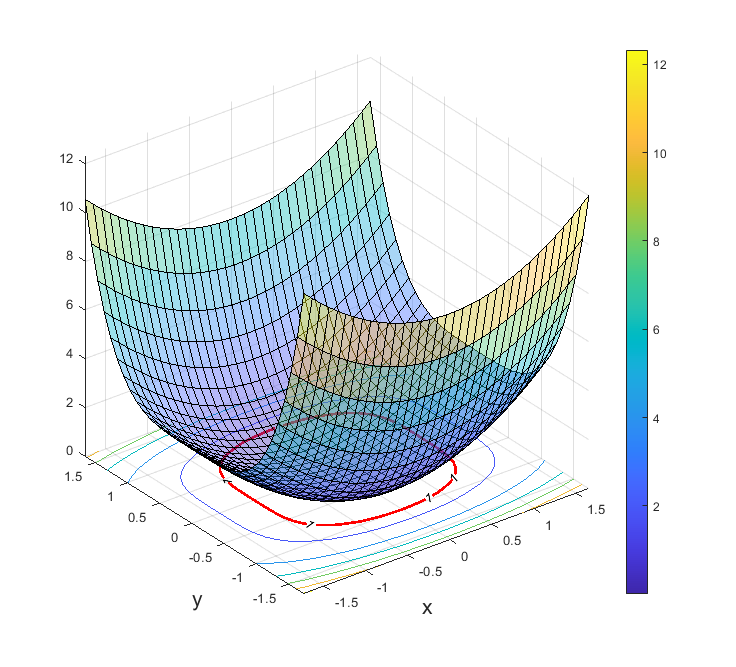
\includegraphics[scale=0.45]{non_convex_SP.png}
    \vspace{-10pt}
    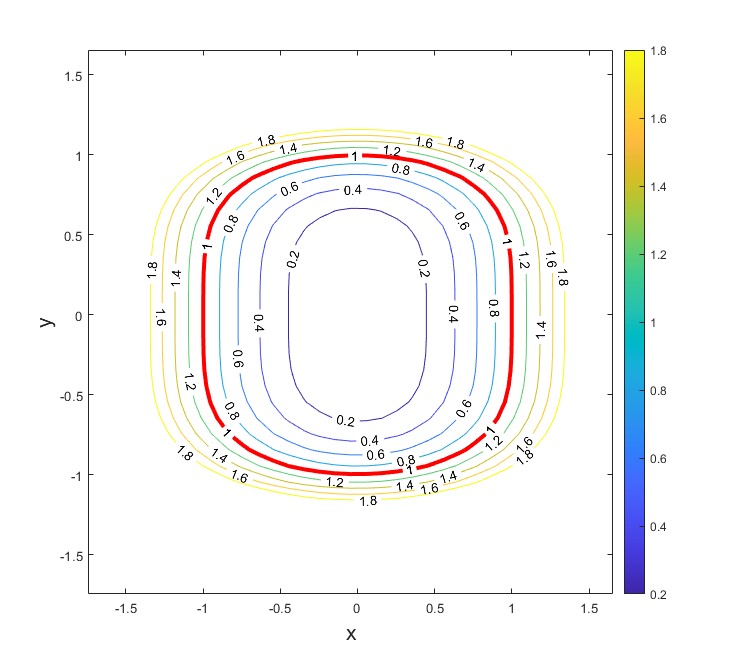
\includegraphics[scale=0.45]{non_convex_SP_levelsets.png}
    %\caption{}
    %\label{fig:convex_SP}
    \end{subfigure}%
    \hspace{-40pt}
    \begin{subfigure}{0.5\textwidth}
    \centering
    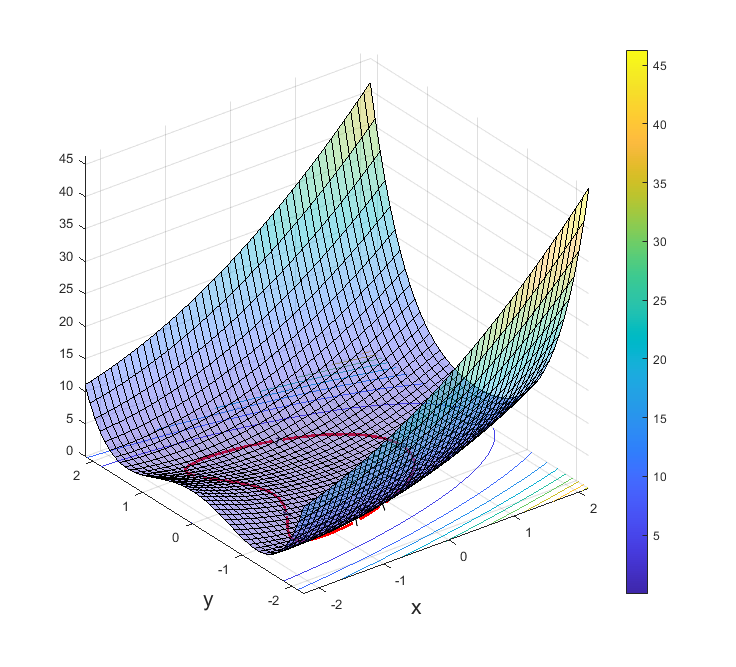
\includegraphics[scale=0.45]{non_convex_S.png}
    \vspace{-10pt}
    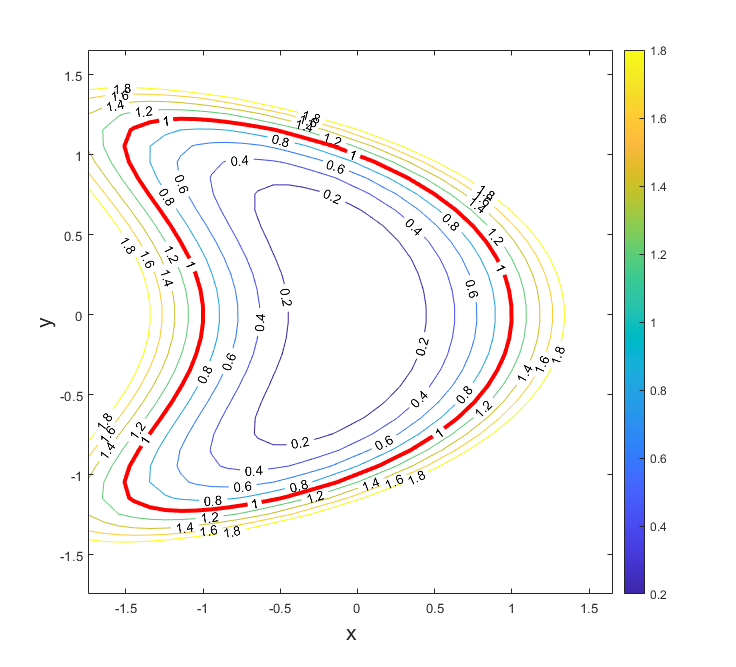
\includegraphics[scale=0.45]{non_convex_S_levelsets.png}
    %\caption{}
    %\label{fig:non_convex_SQ}
    \end{subfigure}
    \caption{$P_1$ and convex $S_{1}$ (red); $P_2$ and non-convex $S_2$ (red)}
    \label{fig:non_convex_SQ}
\end{figure}
\end{example}

\begin{example}\label{exp:Polynomial}\normalfont
 In \cite{Randles2017}, a positive-homogeneous polynomial $P$ is, by definition, a complex-valued multivariate polynomial (on $\mathbb{R}^d$) for which $\Exp(P)$ contains an element of $\End(\mathbb{R}^d)$ whose spectrum is purely real and $R=\Re P$ is positive-definite \textcolor{red}{(See Proposition \ref{prop:PosHomSufficientCondition} below)}. By virtue of Proposition 2.2 of \cite{Randles2017}, for each such polynomial $P$ and $E\in\Exp(P)$ with real spectrum, there exists $A\in\Gl(\mathbb{R}^d)$ (representing a change of basis of $\mathbb{R}^d$) and a $d$-tuple of positive integers $\mathbf{m}=(m_1,m_2,\dots,m_d)\in\mathbb{N}_+^d$ for which $A^{-1}EA$ has standard matrix representation
\begin{equation}\label{eq:DiagonalizableE}
\diag\{(2m_1)^{-1},(2m_2)^{-1},\dots,(2m_d)^{-1}\}
\end{equation}
and
\begin{equation}\label{eq:SemiElliptic}
(P\circ A)(x)=\sum_{|\beta:\mathbf{m}|=2}a_\beta x^\beta
\end{equation}
for $x=(x^1,x^2,\dots,x^d)\in\mathbb{R}^d$; here, for a multi-index $\beta=(\beta_1,\beta_2,\dots,\beta_d)\in\mathbb{N}^d$,
\begin{equation*}
x^{\beta}=(x^1)^{\beta_1}(x^2)^{\beta_2}\cdots (x^d)^{\beta_d} \quad \mbox{and} \quad |\beta:\mathbf{m}|:=\sum_{k=1}^d\frac{\beta_k}{m_k}.
\end{equation*}
Polynomials of the form \eqref{eq:SemiElliptic} are said to be semi-elliptic in the sense of L. H\"{o}rmander and the constant-coefficient partial differential operators they define are hypo-elliptic \cite{Hormander1983}. With the representation \eqref{eq:DiagonalizableE}, it is easy to see that $t^{E}$ is contracting and therefore the real part of each positive-homogeneous polynomial is a positive-homogeneous function by virtue of Condition \ref{cond:ThereExistsContracting} of Proposition \ref{prop:PositiveHomogeneousCharacterization}. It is straightforward to check that the polynomials in Example \ref{exp:non_convex} are positive-homogeneous polynomials of the form \eqref{eq:SemiElliptic}, i.e., semi-elliptic polynomials, with $A=I$. We refer the reader to Section 7.3 of \cite{Randles2017} which presents a positive-homogeneous polynomial which is not semi-elliptic (and so $A\neq I$).
\end{example}

\begin{example}\label{exp:Weierstrass}\normalfont
Let $Q$ be a positive-homogeneous function with exponent set $\Exp(Q)$ and compact level set $S_Q=\{\eta:Q(\eta)=1\}$. Given any $f\in C^0(S_Q)$ for which $f(\eta)>0$ for all $\eta\in S_Q$ and $E\in \Exp(Q)$, define $P=P_{f,Q}:\mathbb{R}^d\to\mathbb{R}$ by
\begin{equation*}
P(x)=\begin{cases}
Q(x)f\left((Q(x)^{-E}x\right) & x\neq 0\\
0 & x=0
\end{cases}
\end{equation*}
for $x\in\mathbb{R}^d$. We claim that $P$ is positive-definite and $\Exp(Q)\subseteq \Exp(P)$.

\begin{subproof}To see this, we first observe that, for any $x\in\mathbb{R}^d\setminus \{0\}$, $Q((Q(x)^{-E}x)=Q(x)/Q(x)=1$ and hence $Q(x)^{-E}x\in S_Q$ and so the above formula makes sense and ensures that $P$ is continuous on $\mathbb{R}^d\setminus\{0\}$. Furthermore, because $f$ is continuous and positive on the compact set $S_Q$, we have $0<\min Q\leq \max Q<\infty$. From this it follows that $P$ must be positive-definite and, by virtue of the squeeze theorem, continuous at $x=0$. Now, given $E\in\Exp(Q)$,
\begin{equation*}
P(t^Ex)=Q(t^Ex)f(Q(t^Ex)^{-E}t^Ex)=tQ(x)f(Q(x)^{-E}x)=tP(x)
\end{equation*}
whenever $x\neq 0$ and $t>0$. It follows that $E\in\Exp(P)$ and, because we know that $t^E$ is contracting, we conclude that $P$ is a positive-homogeneous function in view of Proposition \ref{prop:PositiveHomogeneousCharacterization}. 
\end{subproof}
The utility of this construction allows us to see that ``most'' positive-homogeneous functions are not smooth. To see this, take any positive-definite function $Q\in C^{\infty}(\mathbb{R}^d)$. It follows (See Section \ref{sec:SigmaForSmoothP}) that $S_Q$ is a smooth compact embedded hypersurface of $\mathbb{R}^d$. If $P=P_{f,Q}$ is $C^\infty(\mathbb{R}^d)$, $P\vert_{S_Q}=f$ is necessarily $C^\infty(S_Q)$. It follows that $P\notin C^\infty(\mathbb{R}^d)$ whenever $f$ is chosen from $C^0(S_Q)\setminus C^\infty(S_Q)$. By precisely the same argument, we see that $P\in C^0(\mathbb{R}^d)\setminus C^k(\mathbb{R}^d)$ whenever $f\in C^0(S_Q)\setminus C^k(S_Q)$ for each $k\in\mathbb{N}$.\\

\noindent In looking at the above construction, it should be pointed out that $S_P=\{\eta\in\mathbb{R}^d:P(\eta)=1\}$ does not generally coincide with $S_Q$. In fact, $S_Q=S_P$ if and only if $P=Q$ and (equivalently) $f=1$. As a straightforward example, consider $Q(x,y)=|(x,y)|=\sqrt{x^2+y^2}$ on $\mathbb{R}^2$ with $S_Q=\mathbb{S}$ and define
\begin{equation*}
f(x,y)=w(\mbox{Arg}(x,y))+3
\end{equation*}
where $w:\mathbb{R}\to\mathbb{R}$ is defined by
\begin{equation*}
    w(t) = \sum_{n=0}^\infty 2^{-n} \cos\lp 3^n t \rp
\end{equation*}
for $t\in\mathbb{R}$; this is a continuous $2\pi$-periodic version of the Weierstrass function. The resulting positive-homogeneous function $P$ is continuous but nowhere differentiable. Figure \ref{fig:Weierstrass} illustrates this function $P$ alongside $Q$.


\begin{figure}[!htb]
    \centering
    \hspace{10pt}
    \begin{subfigure}{0.5\textwidth}
    \centering
    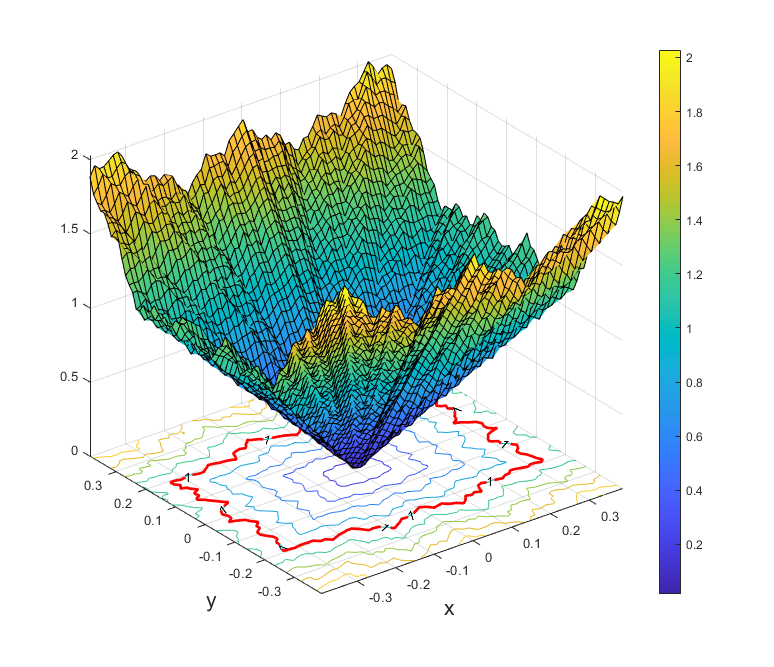
\includegraphics[scale=0.4]{WeierstrassP_and_levelsets.png}
    \vspace{-10pt}
    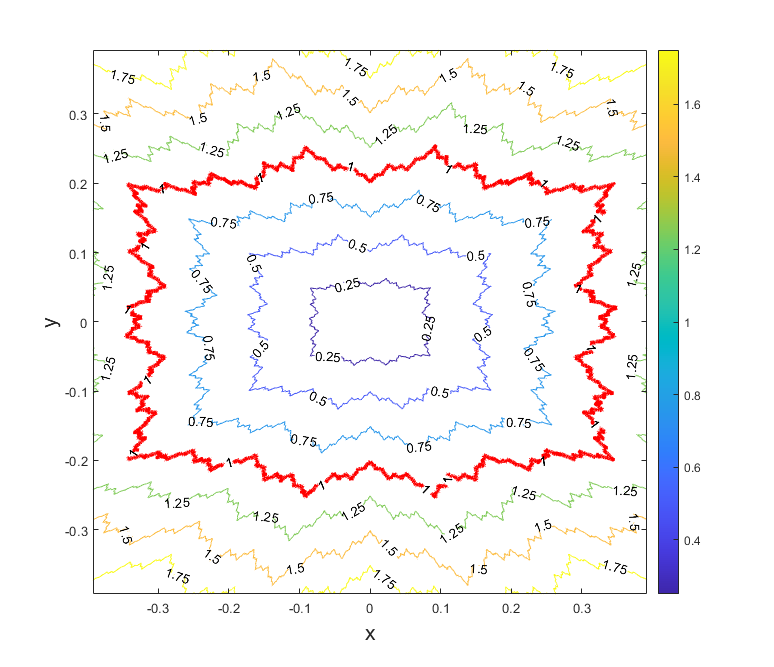
\includegraphics[scale=0.4]{WeierstrassP_levelsets.png}
    %\caption{}
    %\label{fig:WeierstrassP_levelsets}
    \end{subfigure}%
    \hspace{-20pt}
    \begin{subfigure}{0.5\textwidth}
    \centering
    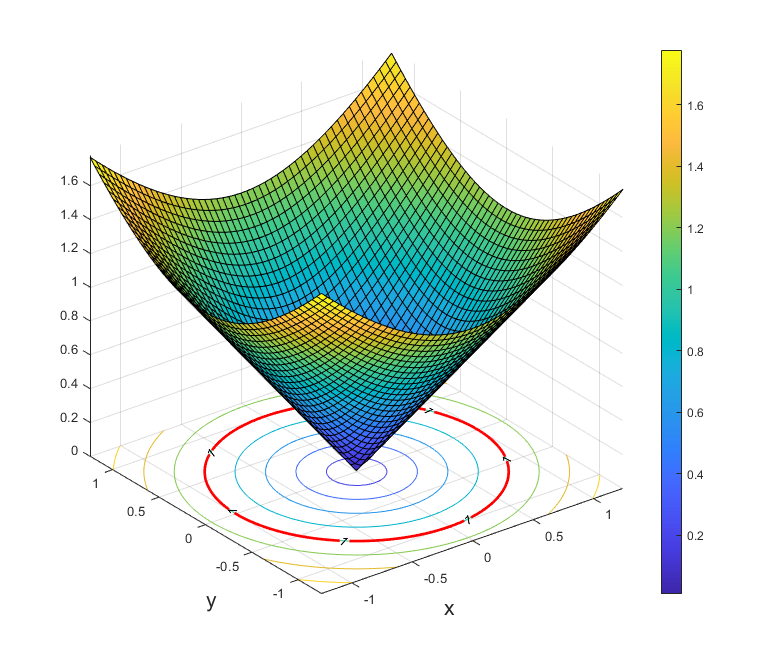
\includegraphics[scale=0.4]{Q_and_levelsets.png}
    \vspace{-10pt}
    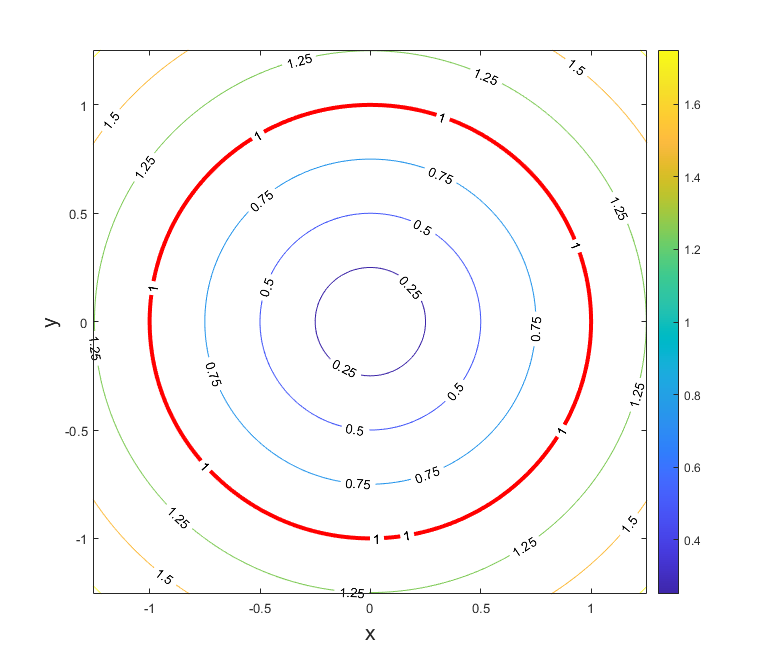
\includegraphics[scale=0.4]{Q_levelsets.png}
    %\caption{}
    %\label{fig:Q_levelsets}
    \end{subfigure}
    \caption{$P$ with $S_P$ highlighted in red; $Q$ with $S_Q$ highlighted in red }
    \label{fig:Weierstrass}
\end{figure}

\end{example}




\noindent For a continuous, positive definite function $P$ for which $\Exp(P)$ is non-empty, the following proposition gives a sufficient condition for $P$ to be positive-homogeneous. As discussed in Example \ref{exp:Weierstrass} above, it is this condition that was used to define ``positive-homogeneous polynomial" in \cite{Randles2017}. \textcolor{red}{We still do not know if this condition is also necessary. See Theorem 1 Part c on Page 178 of \cite{Braun1993}.}



\begin{proposition}\label{prop:PosHomSufficientCondition}
If $P$ is continuous, positive definite and $\Exp(P)$ contains an $E\in\End(\mathbb{R}^d)$ with real spectrum, then $\{t^E\}$ is contracting and hence all of the above conditions are (simultaneously) met. 
\end{proposition}
\begin{proof}
Since $\Spec(E)$ is real, the characteristic polynomial of $E$ factors completely over $\R$ and so we may apply the Jordan-Chevalley decomposition to write $E=S+N$ where $S$ is diagonalizable, $N$ is nilpotent, and $SN=NS$. Let $v_1,v_2,\dots,v_d \in \R^d$ be an eigenbasis of $S$ whose corresponding eigenvalues $\lambda_1,\lambda_2,\dots,\lambda_d$ satisfy $\lambda_k\leq \lambda_{k+1}$ for all $k=1,2\dots,d-1$.

Let us assume, to reach a contradiction, 
that $\{ t^E \}$ is not contracting. Repeating the same argument given in $\ref{cond:PisAboveOne}\Rightarrow\ref{cond:Contracting}$ in the proof of Proposition \ref{prop:PositiveHomogeneousCharacterization}, leaves us with only one possibility: There is a non-zero $x = \sum^d_{i=1}\alpha_i v_i \in\mathbb{R}^d$, and a sequence $t_k\to 0$ for which $|t_k^E x|\to\infty$. Let $n+1$ denote the index of $N$, then we have
\begin{equation*}
t^E_k x = t_k^{N+S} x 
= t_k^N t_k^S x 
= \sum_{j=0}^n\sum_{i=1}^d \f{t_k^{\lambda_i}(\log t_k)^j}{j!}   \alpha_iN^j v_i
\end{equation*}
for all $k$. Since $\abs{t_k^E x} \to \infty$ and $t_k \to 0$, at least one eigenvalue of $S$ must be non-positive. To see this, suppose $\lambda_i > 0$ for all $i = 1,2,\dots,d$, then in view of L'H\^{o}pital's rule we have
\begin{equation*}
    \lim_{t_k \to 0}(\log t_k)^j t_k^{\lambda_i} = 0  
\end{equation*}
for any $j =0, 1,2,\dots,n$ and $i =1,2,\dots,d$, which implies that $\abs{t^E_k x} \not\to \infty$ as $t_k \to 0$, contradicting our assumption. Thus, $\lambda_1 = \min\{ \Spec(S)\} \leq 0$. Let $k$ be such that $N^k v_1 \neq 0$ but $N^{k+1} v_1 = 0$, then
\begin{equation*}
    t^E N^k v_1 = t^S t^N N^k v_1 = t^S \sum_{j=0}^\infty \f{(\log t)^j}{j!}N^j N^k v_1 = t^S N^k v_1 = N^k t^S  v_1 =  t^{\lambda_{1}} N^k  v_1
\end{equation*}
where we have used the fact that $SN = NS$. If $\lambda_1= 0$, then 
\begin{equation*}
    \infty =  \lim_{t\to \infty} tP(N^k v_1)  = \lim_{t\to \infty} P( t^S t^N N^k v_1) =  \lim_{t\to \infty}P(t^{0} N^k v_1)= \lim_{t\to \infty}P( N^k v_1) = P(N^k v_1)
\end{equation*}
which is impossible since $P$ is continuous at $N^k v_1$. On the other hand, if $\lambda_1 < 0$, then
\begin{equation*}
    \infty = \lim_{t\to \infty} tP(N^k v_1) = \lim_{t\to \infty} P(t^S t^N N^k v_1) = \lim_{t\to \infty}P(t^{\lambda_1} N^k v_1) = P(0) = 0
\end{equation*}
which is also impossible. 
\end{proof}




\noindent Given a positive-homogeneous function $P$, let $\Sym(P)$ be the set of $O\in\End(\mathbb{R}^d)$ for which
\begin{equation*}
P(Ox)=P(x)
\end{equation*}
for all $x\in\mathbb{R}^d$. By virtue of the positive-definiteness of $P$, it is easy to see that $\Sym(P)$ is a subgroup of $\Gl(\mathbb{R}^d)$. For this reason, $\Sym(P)$ is said to be the \textit{symmetry group associated to $P$}. 

\begin{proposition}\label{prop:SymCompact}
For each positive-homogeneous function $P$, $\Sym(P)$ is a compact subgroup of $\Gl(\mathbb{R}^d)$. In particular, it is a subgroup of the orthogonal group $O(\mathbb{R}^d)$.
\end{proposition}
\begin{proof}
By virtue of the Heine-Borel theorem (and the fact that $\Gl(\mathbb{R}^d)$ is finite dimensional), we prove that $\Sym(P)$ is closed and bounded. To this end, let $\{O_n\}\subseteq\Sym(P)$ be a sequence converging to $O\in \Gl(\mathbb{R}^d)$. For each $x\in\mathbb{R}^d$, the continuity of $P$ guarantees that
\begin{equation*}
P(Ox)=P\left(\lim_{n\to\infty}O_nx\right)=\lim_{n\to\infty}P(O_nx)=\lim_{n\to\infty}P(x)=P(x).
\end{equation*}
Hence, $O\in\Sym(P)$ and so $\Sym(P)$ is closed.

We assume, to reach a contradiction, that $\Sym(P)$ is not bounded. In this case, there is a sequence $\{\eta_n\}\subseteq \mathbb{S}$ for which $\lim_{n\to\infty}|O_n\eta_n|=\infty$. Given that $\mathbb{S}$ is compact, by passing to a subsequence if needed, we may assume without loss in generality that $\lim_{n\to\infty}\eta_n=\eta\in\mathbb{S}$. By virtue of Proposition \ref{prop:PositiveHomogeneousCharacterization} and the continuity of $P$,
\begin{equation*}
P(\eta)=\lim_{n\to\infty}P(\eta_n)=\lim_{n\to\infty}P(O_n\eta_n)=\infty
\end{equation*}
which is impossible. Hence $\Sym(P)$ is bounded.
\end{proof}

\begin{corollary}\label{cor:TraceisInvariant}
Let $P$ be a positive-homogeneous function, then
\begin{equation*}
\tr E=\tr E'>0
\end{equation*}
for all $E,E'\in\Exp(P)$.
\end{corollary}
\begin{proof}
By virtue of Propositions \ref{prop:ContractingTrace} and \ref{prop:PositiveHomogeneousCharacterization}, $\tr E>0$ for all $E\in\Exp(P)$. It remains to show that the trace map is constant on $\Exp(P)$. To this end, let $E,E'\in\Exp(P)$. Then, for all $t>0$ and $x\in\mathbb{R}^d$,
\begin{equation*}
P(x)=t(1/t)P(x)=tP((1/t)^{E'}x)=P(t^E(1/t)^{E'}x)=P(t^{E}t^{-E'}x).
\end{equation*}
Thus $O_t=t^{E}t^{-E'}\in\Sym(P)$ for each $t>0$. In view of the Propositions \ref{prop:ContinuousGroupProperties} and \ref{prop:SymCompact} and the homomorphism property of the determinant,
\begin{equation*}
1=\det(O_t)=\det(t^{E}t^{E'})=\det(t^{E})\det(t^{-E'})=t^{\tr E}t^{\tr E}=t^{\tr E-\tr E'}
\end{equation*}
for all $t>0$ and therefore $\tr E=\tr E'$.
\end{proof}

\noindent In view of the preceding corollary, to each positive-homogeneous function $P$, we define the \textit{homogeneous order of $P$} to be the unique positive number $\mu_P$ for which
\begin{equation*}
\mu_P=\tr E
\end{equation*}
for all $E\in\Exp(P)$. 

\begin{example}\normalfont The homogeneous orders of the positive-homogeneous functions in Examples \ref{exp:EuclideanNorm}, \ref{exp:non_convex}, \ref{exp:Polynomial}, and \ref{exp:Weierstrass} are given as follows. \ref{exp:EuclideanNorm}: $\mu_{|\cdot|^{\alpha}}=d/\alpha$ for each $\alpha>0$. \ref{exp:non_convex}: $\mu_{P_1}=\mu_{P_2}=3/4$. \ref{exp:Polynomial}: $\mu_P=(2m_1)^{-1}+(2m_2)^{-1}+\cdots+(2m_d)^{-1}$. \ref{exp:Weierstrass}: $\mu_P=\mu_Q$.
\end{example}


\noindent We end this section by addressing a useful proposition which connects $\Exp(P)$ and $\Sym(P)$. Given $O\in\Sym(P)$, we write
\begin{equation*}
    OF=\{O\eta:\eta\in F\}.
\end{equation*}

\begin{proposition}\label{prop:ExpP}
For any  $O \in \Sym{(P)} $
\begin{equation*}
    \Exp(P) = O^\top \Exp(P) O.
\end{equation*}
In other words, the set $\Exp(P)$ is invariant under conjugation by $\Sym(P)$.
\end{proposition}

\begin{proof}
Since $\Sym(P)$ is a subgroup of the orthogonal group $O(\mathbb{R}^d)$, $O^\top = O^{-1} \in \Sym{P}$ whenever $O\in\Sym(P)$. For a fixed $O\in\Sym(P)$, it is easy to see that the map $\Exp(P)\ni E\mapsto  O^\top E O\in\Exp(P)$ is a bijection and hence $\Exp(P)=O^\top \Exp(P) O$. 
% Observe that, if $O^\top E_1 O=O^\top E_2 O$, then by left multiplying by $O$ and right multiplying by $O^T=O^{-1}$ we find that $E_1=E_2$ whence $\mbox{Conj}$ is injective.
% Now, if $E_i, E_j\in \Exp(P)$ and $E_i\neq E_j$, then $O^\top E_i O \neq O^\top E_j O$ since $O,O^\top\in \OdR{}$. Thus the conjugation map induced by $O$, $\varphi_O: \Exp{P}\to \Exp{P}$ defined by 
% \begin{equation*}
%     \varphi_O (E) = O^\top E O
% \end{equation*}
% is one-to-one. Further, for any $E\in \Exp(P)$, a similar argument as \eqref{eq:OOO} shows that $OEO^\top \in \Exp(P)$ and satisfies
% \begin{equation*}
%     \varphi_O(OEO^\top) = O^\top (OEO^\top) O = E\in \Exp{(P)}.
% \end{equation*}
% So, $\varphi_O$ is bijective, which means 
% \begin{equation*}
%     \Exp(P) = O^\top \Exp(P) O = O \Exp{(P)} O^\top, \quad \text{for all } O\in \Sym{(P)}.
% \end{equation*}
\end{proof}

\subsection{Subhomogeneous functions}\label{subsec:SubhomogeneousFunctions}
In this subsection, we introduce the notions of subhomogeneous functions and strongly subhomogeneous functions with respect to a given endomorphism $E\in\End(\mathbb{R}^d)$. When studying convolutions powers of a general complex-valued function $\phi$ on $\mathbb{Z}^d$, along with positive homogeneous polynomials, such functions are commonly seen in \textcolor{red}{Taylor expansions of the Fourier transform of $\widehat{\phi}$} \textcolor{blue}{I think this should be $\Gamma$}. Though the content of this subsection naturally follows the preceding treatment of positive-homogeneous  functions, we shall not make use of this material until Section \ref{sec:ConvolutionPowers}. The reader should feel free to delay reading this subsection until \textcolor{red}{he/she/they} is ready to read Section \ref{sec:ConvolutionPowers}.

\begin{definition}\label{def:homogeneous_types}
Let $Q$ be a complex-valued function defined on an open neighborhood of $0$ in $\mathbb{R}^d$ and let $E\in\End(\mathbb{R}^d)$ be such that $\{r^E\}$ is a contracting group.
\begin{enumerate}
\item We say that $Q$ is \textbf{subhomogeneous} with respect to $E$ if, for each $\epsilon>0$ and compact set $K$, there is a $\delta>0$ for which
\begin{equation*}
\abs{Q(r^E\xi)}\leq \epsilon r
\end{equation*}
for all $0<r<\delta$ and $\xi\in K$.
\item In the case that $Q$ is differentiable on its domain, we say that $Q$ is \textbf{strongly subhomogeneous} with respect to $E$ if, for each $\epsilon>0$ and compact set $K$, there is a $\delta>0$ for which
\begin{equation*}
\abs{\partial_r Q(r^E\xi)}\leq \epsilon
\end{equation*}
for all $0<r<\delta$ and $\xi\in K$.
\end{enumerate}
\end{definition}

\begin{proposition}\label{prop:supersub_implies_sub}
Let $Q$ be differentiable on an open neighborhood of $0$ in $\mathbb{R}^d$ and let $E\in\End(\mathbb{R}^d)$ be such that $\{r^E\}$ is a contracting group. If $Q$ is strongly subhomogeneous with respect to $E$ and $Q(0)=0$, then $Q$ is subhomogeneous with respect to $E$.
\end{proposition}
\begin{proof}
Let $\epsilon>0$ and $K$ be a compact set.  In view of our supposition that $Q$ is strongly subhomogeneous with respect to $E$, let $\delta>0$ be given so that $\abs{\partial_r Q(r^E\xi)}\leq \epsilon$ for all $\xi\in K$ and $0<r< \delta$. Given that $r^E$ is a contracting group and $Q(0)=0$, it follows that, for each $\xi\in K$, $f_{\xi}:[0,\delta)\to\mathbb{C}$ defined by
\begin{equation*}
f_{\xi}(r)=\begin{cases}
Q(r^E\xi) & 0<r<\delta\\
0 & r=0
\end{cases}
\end{equation*}
is differentiable on $(0,\delta)$ and continuous on $[0,\delta)$, for each $\xi\in K$. Consequently, for every $0<r<\delta$ and $\xi\in K$, the mean value theorem guarantees a $c=c_{\xi,r}\in (0,r)$ for which 
\begin{equation*}
\abs{f_{\xi}(r)-f_{\xi}(0)}\leq r\abs{f_{\xi}'(c)}=r\abs{\partial_r Q(c^E\xi)}\leq r\epsilon.
\end{equation*}
Consequently, for all $0<r<\delta$ and $\xi\in K$,
\begin{equation*}
\abs{Q(r^E\xi)}=\abs{f_{\xi}(r)-f_{\xi}(0)}\leq r\epsilon.
\end{equation*}
\end{proof}

\textcolor{red}{We may not need this at all} The following result will be helpful in establishing estimates using the Van der Corput lemma; its proof is straightforward and omitted.
\begin{lemma}\label{lem:ScalingofSubHomogeneous}
Let $Q$ be a complex-valued function defined on a neighborhood of $0$, $E\in\End(\mathbb{R}^d)$ be such that $r^E$ is contracting, and $k>0$.
\begin{enumerate}
\item If $Q$ is subhomogeneous with respect to $E/k$, then, for each $\epsilon>0$ and compact set $K$, there is a $\delta>0$ for which 
\begin{equation*}
\abs{Q(r^{E}\xi)}\leq \epsilon r^k
\end{equation*}
for all $0<r<\delta^k$ and $\xi\in K$.
\item If $Q$ is strongly subhomogeneous with respect to $E/k$, then, for each $\epsilon>0$ and compact set $K$, there is $\delta>0$ for which
\begin{equation*}
\abs{\partial_r Q(r^E\xi)}\leq \epsilon k  r^{k-1}
\end{equation*}
for all $0<r<\delta^k$ and $\xi\in K$.
\end{enumerate}
\end{lemma}
\begin{proof}
Let $Q$ be subhomogeneous with respect to $E/k$. Then, for each $\epsilon > 0$ and compact set $K$, Definition \ref{def:homogeneous_types} guarantees a $\delta> 0$ for which 
$\abs{Q(\theta^{E/k} \xi)} \leq \epsilon \theta$ for all $0 < \theta < \delta$ and $\xi \in K$. For $r = \theta^{1/k}$, we have $0<r<\delta^k$ whenever $0<\theta<\delta$. Consequently,
\begin{equation*}
    \abs{Q(r^E \xi)} =\abs{Q(\theta^{E/k}\xi)} \leq \epsilon \theta= \epsilon r^k
\end{equation*}
for all $0 < r < \delta^k$ and $\xi \in K$. 

Assume additionally that $Q$ is strongly subhomogeneous with respect to $E/k$. Let $\epsilon > 0$ and a compact set $K$ be given. Definition \ref{def:homogeneous_types} guarantees a $\delta> 0$ for which $\abs{\p_\theta Q(\theta^{E/k} \xi)} \leq \epsilon$ for all $\xi \in K$ and $0 < \theta < \delta$. As before, for $r = \theta^{1/k}$, we have $0<r<\delta^k$ whenever $0<\theta<\delta$. Consequently, the chain rule guarantees that
\begin{equation*}
    \abs{\p_r Q(r^{E} \xi)} = \abs{\p_\theta Q(\theta^{E/k} \xi)} 
    \abs{\f{\p \theta}{\p r}} \leq \epsilon k  r^{k-1}
\end{equation*}
for all $0 < r < \delta^k$ and $\xi \in K$. 
\end{proof}

\begin{proposition}\label{prop:Subhomequivtolittleoh}
Let $P$ be positive-homogeneous and $\widetilde{P}$ be complex-valued and continuous on a neighborhood of $0$ in $\mathbb{R}^d$. The following are equivalent:
\begin{enumerate}[label=(\alph*), ref=(\alph*)]
    \item\label{item:Subhomequivtolittleoh1} $\widetilde{P}(\xi)=o(P(\xi))$ as $\xi\to 0$.
    \item\label{item:Subhomequivtolittleoh2} For every $E\in\Exp(P)$, $\widetilde{P}$ is subhomogeneous with respect to $E$.
    \item\label{item:Subhomequivtolittleoh3} There exists $E\in\Exp(P)$ for which $\widetilde{P}$ is subhomogeneous with respect to $E$.
\end{enumerate}
\end{proposition}
\begin{proof}
\begin{subproof}[\ref{item:Subhomequivtolittleoh1} $\Rightarrow$ \ref{item:Subhomequivtolittleoh2}] Let $\epsilon>0$, $K$ be a compact set and choose $E\in \Exp(P)$. Given our supposition that $\widetilde{P}(\xi)=o(P)(\xi)$ as $\xi\to 0$, we can find an open neighborhood $\mathcal{O}$ of $0$ for which 
\begin{equation*}
\abs{\widetilde{P}(\xi)}\leq \frac{\epsilon}{1+\sup_{\eta\in K}P(\eta)}P(\xi)
\end{equation*}
for all $\xi\in \mathcal{O}$. Now, because $r^E$ is contracting in view of Proposition \ref{prop:PositiveHomogeneousCharacterization}, we can find a $\delta>0$ for which $r^E\xi\in \mathcal{O}$ for all $0<r<\delta$ and $\xi\in K$ by virtue of Proposition \ref{prop:ContractingCapturesCompact}. Consequently, for all $0<r<\delta$ and $\xi\in K$,
\begin{equation*}
\abs{\widetilde{P}(r^E\xi)}\leq \frac{\epsilon}{1+\sup_{\eta\in K}P(\eta)}P(r^E\xi)=\epsilon r\frac{P(\xi)}{1+\sup_{\eta\in K}P(\eta)}\leq r\epsilon.
\end{equation*}
\end{subproof}

\begin{subproof} [\ref{item:Subhomequivtolittleoh2} $\Rightarrow$ \ref{item:Subhomequivtolittleoh3}] This implication is trivial.
\end{subproof}
 
 \begin{subproof}[\ref{item:Subhomequivtolittleoh3} $\Rightarrow$ \ref{item:Subhomequivtolittleoh1}]  Let $\epsilon>0$. Choose $E\in \Exp(P)$ and let $S=\{\eta\in\mathbb{R}^d:P(\eta)=1\}$. Using the supposition that $\widetilde{P}$ is subhomogeneous with respect to $E$, we may choose $\delta>0$ for which
\begin{equation*}
\abs{\widetilde{P}(r^E\eta)}\leq \epsilon r 
\end{equation*}
 for all $0<r<\delta$ and $\eta\in S$. We remark that, in view of the continuity of $\widetilde{P}$ and the fact that $r^E$ is contracting, this inequality ensures that $\widetilde{P}(0)=0$. We set $\mathcal{O}=\{0\}\cup \psi_E((0,\delta)\times S)$, which is necessarily an open set by virtue of Proposition \ref{prop:PsiHomeomorphism}. Then, for every $\xi=r^E\eta \in\mathcal{O}\setminus\{0\}$, 
\begin{equation*}
\abs{\widetilde{P}(\xi)}=\abs{\widetilde{P}(r^E\eta)}\leq r\epsilon=\epsilon rP(\eta)=\epsilon P(r^E\eta)=\epsilon P(\xi)
\end{equation*}
If $\xi=0$, obviously, $\abs{\widetilde{P}(\xi)}=0=\epsilon P(0)=\epsilon P(\xi)$. Thus, for all $\xi\in\mathcal{O}$,
\begin{equation*}
\abs{\widetilde{P}(\xi)}\leq\epsilon P(\xi),
\end{equation*}
as desired.
\end{subproof}
\end{proof}



\section{A surface measure on $S$ and a generalized polar integration formula}\label{sec:IntegrationFormula}

This section is dedicated to constructing a surface measure on the the compact level set $S$ associated to a positive-homogeneous function and using it to generalize the polar integration formula \eqref{eq:StandardPolarIntegrationFormula}. To introduce our main theorem, let $P$ be a positive-homogeneous function with homogeneous order $\mu_P>0$, exponent set $\Exp(P)$ and symmetry group $\Sym(P)$. We shall denote by $\mathcal{M}_d$ the Lebesgue $\sigma$-algebra on $\mathbb{R}^d\setminus\{0\}$ and by $m$ the Lebesgue measure.  Also, let the compact set $S=S_P=\{\eta\in\mathbb{R}^d:P(\eta)=1\}$ in $\mathbb{R}^d$ be equipped with its relative topology and denote by $\mathcal{B}(S)$ the Borel $\sigma$-algebra on $S$. We denote by $\mathcal{L}=\mathcal{L}(0,1)$ the $\sigma$-algebra of Lebesgue measureable sets on $(0,\infty)$ and let $\lambda_P$ be the $\sigma$-finite measure on $((0,\infty),\mathcal{L})$ with $\lambda_P(dt)=t^{\mu_P-1}\,dt$. Our main theorem is as follows\footnote{We refer the reader to Section 3.6 and 9.2 of \cite{Bogachev2007} which provides some basic context and vocabulary.}. 

\textcolor{red}{\noindent Throughout this section, $P$ denotes a fixed positive-homogeneous function on $\mathbb{R}^d$ with homogeneous order $\mu_P>0$ and exponent set $\Exp(P)$. We will take $S=S_P=\{\eta\in\mathbb{R}^d:P(\eta)=1\}$ to be equipped with the relative topology inherited from $\mathbb{R}^d$ and, given $(0,\infty)$ with its usual topology, we take $(0,\infty)\times S$ to be equipped with the product topology. }


\begin{theorem}\label{thm:BestIntegrationFormula}
There exists a $\sigma$-algebra $\Sigma$ on $S$ containing $\mathcal{B}(S)$ and a finite Radon measure $\sigma_P$ on $(S,\Sigma)$ which satisfies the following properties:
\begin{enumerate}
\item\label{property:Completion} $(S,\Sigma,\sigma_P)$ is the completion of $(S,\mathcal{B}(S),\sigma_P)$. In particular, $(S,\Sigma,\sigma_P)$ is a complete measure space.
\item\label{property:Invariance} For any $F\in\Sigma$ and $O\in\Sym(P)$, $\sigma(OF)=\sigma(F)$.
\item\label{property:DefiningConditionofsigma} For any $F\in\Sigma$ and $E\in\Exp(P)$, 
\begin{equation*}
\widetilde{F_E}:=\bigcup_{0<t<1}\left(t^E F\right)=\left\{t^E\eta\in\mathbb{R}^d\setminus\{0\}:0<t<1,\eta\in F\right\}
\end{equation*}
is a Lebesgue measurable subset of $\mathbb{R}^d\setminus \{0\}$, i.e., $\widetilde{F_E}\in\mathcal{M}_d$, and
\begin{equation*}
\sigma_P(F)=\mu_P\cdot m\left(\widetilde{F_E}\right)
\end{equation*}
where $m$ denotes the Lebesgue measure on $\mathbb{R}^d$.
\end{enumerate}
\textcolor{red}{Is Property \ref{property:Invariance} characterizing? If so, it would be nice to rephrase the above as: There is a unique Radon measure..... \\}
Further, denote by $\left((0,\infty),\times S,(\mathcal{L}\times\Sigma)',\lambda_P\times\sigma_P\right)$ the completion of the product measure space $((0,\infty\times S,\mathcal{L}\times\Sigma,\lambda_P\times\sigma_P)$. We have
\begin{enumerate}
\item\label{property:BestPointIsomorphism} Given any $E\in \Exp(P)$, the map $\psi_E:(0,\infty)\times S\to\mathbb{R}^d\setminus\{0\}$, defined by $\psi_E(t,\eta)=t^E\eta$ for $t>0$ and $\eta\in S$, is a point isomorphism of the measure spaces $\left((0,\infty)\times S,(\mathcal{L}\times\Sigma)',\lambda_P\times\sigma_P\right)$ and $(\mathbb{R}^d\setminus\{0\},\mathcal{M}_d,m)$. That is
\begin{equation*}
\mathcal{M}_d=\left\{A\subseteq \mathbb{R}^d\setminus\{0\}:\psi_E^{-1}(A)\in (\mathcal{L}\times\Sigma)'\right\}
\end{equation*}
and, for each $A\in\mathcal{M}_d$,
\begin{equation*}
m(A)=(\lambda_P\times\sigma_P)(\psi_E^{-1}(A)).
\end{equation*}
\item\label{property:BestIntegrationFormula} Given any Lebesgue measureable function $f:\mathbb{R}^d\to\mathbb{C}$ and $E\in \Exp(P)$, $f\circ \psi_E$ is $(\mathcal{L}\times\Sigma)'$-measurable and the following statements hold:
\begin{enumerate}
\item If $f\geq 0$, then
\begin{equation}\label{eq:BestIntegrationFormula}
\int_{\mathbb{R}^d}f(x)\,dx=\int_0^\infty\left(\int_S f(t^E\eta)\,\sigma_P(d\eta)\right)t^{\mu_P-1}\,dt=\int_S\left(\int_0^\infty f(t^E\eta)t^{\mu_P-1}\,dt\right)\sigma_P(d\eta).
\end{equation}
\item When $f$ is complex-valued, we have 
\begin{equation*}f\in L^1(\mathbb{R}^d)\hspace{.5cm}\mbox{ if and only if}\hspace{.5cm}f\circ\psi_E\in L^1\left((0,\infty)\times S,(\mathcal{L}\times\Sigma)',\lambda_P\times\sigma_P\right)
\end{equation*} 
and, in this case, \eqref{eq:BestIntegrationFormula} holds.
\end{enumerate}
\end{enumerate}
\end{theorem}
\noindent As \eqref{eq:StandardPolarIntegrationFormula} finds utility in the harmonic analysis of radial functions, i.e., those functions of the form $f(x)=f_0(|x|)$, Theorem \ref{thm:BestIntegrationFormula} will aid the analysis of functions of the form $f(x)=f_0(P(x))$. In fact, this is a primary motivation for our work. \textcolor{red}{(More needed)}\\

\noindent Our construction proceeds as follows. In Subsection \ref{subsec:ConstructionofSigma}, we fix $E\in\Exp(P)$ and consider the one-parameter contracting group $\{t^E\}$. As the standard isotropic one-parameter group $t\mapsto tI=t^I$ is well-fitted to the unit sphere $\mathbb{S}$ and allows every non-zero $x\in\mathbb{R}^d$ to be written uniquely as $x=t\eta$ for $t\in (0,\infty)$ and $\eta\in \mathbb{S}$, $\{t^E\}$ is well-fitted to to $S$ and has the property that every non-zero $x\in\mathbb{R}^d$ can be written uniquely as $x=t^E\eta$ where $t\in(0,\infty)$ and $\eta\in S$. With this one-parameter group as a tool, we define a \textit{surface-carried}\footnote{\textcolor{red}{We really need to see if this is standard vocabulary}} measure $\sigma_{P,E}$ on $S$ by taking sufficiently nice sets $F\subseteq S$, stretching them into a quasi-conical region of the associated ``ball" $B$ with the contracting group $\{t^E\}$, and computing the Lebesgue measure of the result. In Subsection \ref{subsec:ProductMeasure}, we turn our focus to an associated product measure $\lambda_P\times\sigma_{P,E}$ on $(0,\infty)\times S$ with which we are able to formulate and prove a generalization of \eqref{eq:StandardPolarIntegrationFormula}; this is Theorem \ref{thm:MainIntegrationFormula}. We then derive a number of corollaries of Theorem \ref{thm:MainIntegrationFormula}, including the result that $\sigma_{P,E}$ is a Radon measure on $S$. As everything done in Subsections \ref{subsec:ConstructionofSigma} and \ref{subsec:ProductMeasure} is done using the contracting group $\{t^E\}$ for a chosen $E\in\Exp(P)$, it isn't clear, a priori, exactly how $\sigma_{P,E}$ is dependent on the choice of $E\in\Exp(P)$, if at all. In Subsection \ref{subsec:IndependentofE}, we prove that $\sigma_{P,E}$ is, in fact, independent of the choice of $E\in \Exp(P)$ (and so we write $\sigma_P=\sigma_{P,E}$ and this quickly yields a stronger version of Theorem \ref{thm:MainIntegrationFormula}; this is Theorem \ref{thm:BestIntegrationFormula}. All throughout this section, our construction uses only tools from point-set topology and measure theory.  In Section \ref{sec:SigmaForSmoothP}, we study the special case in which a positive-homogeneous function $P$ is additionally smooth. In that case, we will find that $S$ is a smooth compact embedded hypersurface of $\mathbb{R}^d$ and the measure $\sigma$ is closely related to the Riemannian volume on $S$; see Theorem \ref{thm:RiemannLebesgue}.\\


Before we move to construct $\sigma_P$, we address a useful corollary.  
\begin{corollary}\label{cor:IntegrateOnS}
Given $g:S\to\mathbb{C}$ and $E\in\Exp(P)$, define $f:\mathbb{R}^d\setminus \{0\}\to\mathbb{C}$ defined by
\begin{equation*}
f(x)=\mu_P\cdot \chi_{(0,1)}(P(x))g(P(x)^{-E}x)
\end{equation*}
for $x\in\mathbb{R}^d\setminus\{0\}$. If $g\in L^1(S,\Sigma_P,\sigma_p)$, then $f\in L^1(\mathbb{R}^d\setminus\{0\})$, and 
\begin{equation*}
    \int_{\mathbb{R}^d}f(x)\,dx=\int_Sg(\eta)\sigma_P(d\eta).
\end{equation*}
\end{corollary}
\begin{proof}
Observe that, for the $(\mathcal{L}\times\Sigma_P)'$-measurable function $k(t,\eta)=\chi_{(0,1)}(t)g(\eta)$,
\begin{equation*}
    k\circ\psi_E^{-1}(x)=k(P(x),P(x)^{-E}x)=f(x)
\end{equation*}
for $x\in\mathbb{R}^d\setminus \{0\}$. By virtue of Theorem \ref{thm:BestIntegrationFormula}, it follows that $f$ is $\mathcal{M}_d$ measurable and 
\begin{eqnarray*}
   \int_{\mathbb{R}^d}|f(x)|\,dx&=&\int_{S}\left(\int_{(0,\infty)}|k(t,\eta)|t^{\mu_P-1}\,dt\right)\sigma_P(d\eta)\\
    &=&\left(\int_S|g(\eta)|\sigma_P(d\eta)\right)\left(\int_0^1 \mu_P t^{\mu_P-1}\,dt\right)=\|g\|_{L^1(\sigma_P)}<\infty.
\end{eqnarray*}
Therefore, by an analogous computation (for $f$ instead of $|f|$), we have
\begin{equation*}
    \int_{\mathbb{R}^d}f(x)\,dx=\int_S g(\eta)\sigma_P(d\eta),
\end{equation*}
by virtue of Property \ref{property:BestIntegrationFormula} of Theorem \ref{thm:BestIntegrationFormula}. 
\end{proof}










\subsection{Construction of $\sigma_{P,E}$}\label{subsec:ConstructionofSigma}

Throughout this section, we fix $E\in\Exp(P)$. Define $\psi_E:(0,\infty)\times S\to\mathbb{R}^d\setminus\{0\}$ by
\begin{equation}\label{eq:Homeomorphism}
\psi_E(t,\eta)=t^E\eta
\end{equation}
for $t>0$ and $\eta\in S$. As $\psi_E$ is the restriction of the continuous function $(0,\infty)\times \mathbb{R}^d\ni (t,x)\mapsto t^E x\in\mathbb{R}^d$ to $(0,\infty)\times S$, it is necessarily continuous. As the following proposition shows, $\psi_E$ is, in fact, a homeomorphism.

\begin{proposition}\label{prop:PsiHomeomorphism}
The map $\psi_E:(0,\infty)\times S\to\mathbb{R}^d\setminus\{0\}$ is a homeomorphism with continuous inverse $\psi_E^{-1}:\mathbb{R}^d\setminus\{0\}\to (0,\infty)\times S$ given by
\begin{equation*}
\psi_E^{-1}(x)=(P(x),(P(x))^{-E}x)
\end{equation*}
for $x\in\mathbb{R}^d\setminus\{0\}$.
\end{proposition}

\begin{proof}
Given that $P$ is continuous and positive-definite, $P(x)>0$ for each $x\in \mathbb{R}^d\setminus\{0\}$ and the map $\mathbb{R}^d\setminus\{0\}\ni x \mapsto (P(x))^{-E}x\in \mathbb{R}^d$ is continuous. Further, in view of the homogeneity of $P$,
\begin{equation*}
P\left((P(x))^{-E}\xi\right)=P(x)^{-1}P(x)=1
\end{equation*}
for all $x\in\mathbb{R}^d\setminus\{0\}$. It follows from these two observations that
\begin{equation*}
\rho(x)=(P(x),(P(x))^{-E}x),
\end{equation*}
defined for $x\in\mathbb{R}^d\setminus\{0\}$, is a continuous function taking $\mathbb{R}^d\setminus\{0\}$ into $(0,\infty)\times S$. We have
\begin{equation*}
(\psi_E\circ \rho)(x)=\psi_E(P(x),(P(x))^{-E}x)=(P(x))^{E}(P(x))^{-E}x=x
\end{equation*}
for every $x\in \mathbb{R}^d\setminus \{0\}$ and
\begin{equation*}
(\rho\circ\psi_E)(t,\eta)=\rho(t^E\eta)=(P(t^{E}\eta),(P(t^{E}\eta))^{-E}(t^E\eta))=(tP(\eta),(tP(\eta))^{-E}(t^{E}\eta))=(t,\eta)
\end{equation*}
for every $(t,\eta)\in (0,\infty)\times S$. Thus $\rho$ is a (continuous) inverse for $\psi_E$ and so it follows that $\psi_E$ is a homeomorphism and $\rho=\psi_E^{-1}$.
\end{proof}



\noindent We shall now construct the $\sigma$-algebra $\Sigma_{P,E}$ on $S$; later, we will show that it is independent of our choice of $E$. As in the statement of Theorem \ref{thm:BestIntegrationFormula}, for each $F\subseteq S$, define
\begin{equation*}
\widetilde{F_E}=\bigcup_{0<t<1}\left(t^E F\right)=\{t^E\eta:0<t<1,\eta\in F\}. 
\end{equation*}
We shall denote by $\Sigma_{P,E}$ the collection of subsets $F$ of $S$ for which $\widetilde{F_E}\in\mathcal{M}_d$, i.e.,  
\begin{equation*}
\Sigma_{P,E}=\{F\subseteq S:\widetilde{F_E}\in\mathcal{M}_d\}.
\end{equation*}


\begin{proposition}\label{prop:BorelContainment}
$\Sigma_{P,E}$ is a $\sigma$-algebra on $S$ containing the Borel $\sigma$-algebra on $S$, $\mathcal{B}(S)$.
\end{proposition}

\begin{proof}
Throughout the proof, we write $\Sigma=\Sigma_{P,E}$ and $\widetilde{F}=\widetilde{F_E}$ for each $F\subseteq S$.
We first show that $\Sigma$ is a $\sigma$-algebra. Since $\widetilde S=B\setminus\{0\}$, it is open in $\mathbb{R}^d\setminus\{0\}$ and therefore Lebesgue measurable. Hence $S\in \Sigma$. Let $G, F\in \Sigma$ be such that $G\subseteq F$. Then,
\begin{equation*}
\widetilde{F\setminus G}=\bigcup_{0<t<1}t^E\left(F\setminus G\right)=\bigcup_{0<t<1}\left(t^EF\setminus t^E G\right)=\left(\bigcup_{0<t<1}t^E F\right)\setminus\left(\bigcup_{0<t<1}t^E G\right)=\widetilde F\setminus \widetilde G
\end{equation*}
where we have used the fact that the collection $\{t^E F\}_{0<t<1}$ is mutually disjoint to pass the union through the set difference. Consequently $\widetilde F\setminus \tilde{G}$ is Lebesgue measurable and therefore $F\setminus G\in \Sigma$.  Now, given a countable collection $\{F_n\}\subseteq \Sigma_S$, observe that
\begin{equation*}
    \widetilde{\bigcup_{n=1}^\infty F_n}= \bigcup_{0<t<1} t^E \left(\bigcup_{n=1}^\infty F_n\right)= \bigcup_{0 <t < 1}  \bigcup_{n=1}^\infty  t^E F_n =\bigcup_{n=1}^\infty \bigcup_{0 <t < 1}  t^E F_n =\bigcup_{n=1}^\infty \widetilde{F_n} \in \mathcal{M}_d
\end{equation*}
whence $\cup_n F_n\in \Sigma_S$. Thus $\Sigma$ is a $\sigma$-algebra. 

Finally, we show that
\begin{equation*}
\mathcal{B}(S)\subseteq\Sigma.
\end{equation*}
As the Borel $\sigma$-algebra is the smallest $\sigma$-algebra containing the open subsets of $S$, it suffices to show that $\mathcal{O}\in \Sigma$ whenever $\mathcal{O}$ is open in $S$. Armed with Proposition \ref{prop:PsiHomeomorphism}, this is an easy task: Given an open set $\mathcal{O}\subseteq S$, observe that
\begin{equation*}
\widetilde{\mathcal{O}}=\{t^E\eta:0<t<1,\eta\in\mathcal{O}\}=\psi_E((0,1)\times\mathcal{O}).
\end{equation*}
Upon noting that $(0,1)\times\mathcal{O}$ is an open subset of $(0,\infty)\times S$, Proposition \ref{prop:PsiHomeomorphism} guarantees that $\widetilde{\mathcal{O}}=\psi_E((0,1)\times\mathcal{O})\subseteq\mathbb{R}^d\setminus\{0\}$ is open and therefore Lebesgue measurable. Thus $\mathcal{O}\subseteq \mathcal{M}_d$.
\end{proof}

\noindent We are now ready to specify a measure on the measurable space $(S,\Sigma_{P,E})$. For each $F\in \Sigma_{P,E}$, we define
\begin{equation*}
\sigma_{P,E}(F)=\mu_P\cdot m(\widetilde{F_E})
\end{equation*}
where $m$ is the Lebesgue measure on $\mathbb{R}^d$ and $\mu_P=\tr E>0$ is the homogeneous order associated to $P$.

\begin{proposition}\label{prop:sigmaisameaure}
$\sigma_{P,E}$ is a finite measure on $(S,\Sigma_{P,E})$.
\end{proposition}
\begin{proof}

\noindent Throughout the proof, we will write $\sigma=\sigma_{P,E}$, $\Sigma=\Sigma_{P,E}$, and, $\widetilde{F}=\widetilde{F_E}$ for each $F\subseteq S$. It is clear that $\sigma$ is non-negative and $\sigma(\varnothing)=0$ because $\widetilde{\varnothing}=\varnothing$. Let $\{ F_n  \}^\infty_{n=1} \subseteq \Sigma $ be a mutually disjoint collection. We claim that $\{ \widetilde{F_n} \}_{n=1}^\infty\subseteq\mathcal{M}_d$ is also a mutually disjoint collection. To see this, suppose that $x = t_n^E \eta_n = t_m^E \eta_m\in \widetilde{F_n}\cap\widetilde{F_m}$, where $t_n,t_m \in (0,1)$, $\eta_n \in F_n$, and $\eta_m \in F_m $. Then
\begin{equation*}
    t_n = P(t_n^E \eta_n) = P(x) = P(t_m^E \eta_m) = t_m,
\end{equation*}
implying that $\eta_n = \eta_m\in F_n\cap F_m$. Because $\{F_n\}_{n=1}^\infty$ is mutually disjoint, we must have $n=m$ which verifies our claim. By virtue of the countable additivity of Lebesgue measure, we therefore have
\begin{equation*}
\sigma\left(\bigcup_{n=1}^\infty F_n\right)
    = \mu_P\cdot m\left( \widetilde{\bigcup^\infty_{n=1} F_n } \right)=\mu_P\cdot m\left( \bigcup^\infty_{n=1}\widetilde{F_n} \right)
    = \mu_P\sum^\infty_{n=1} m(\widetilde{F_n})
    = \sum^\infty_{n=1}\sigma(F_n).
\end{equation*}
Therefore $\sigma$ is a measure on $(S,\Sigma)$. In view of Condition \ref{cond:PisAboveOne} of Proposition \ref{prop:PositiveHomogeneousCharacterization}, $\widetilde{S}=B\setminus\{0\}$ is a bounded subset of $\mathbb{R}^d\setminus\{0\}$ and hence $\sigma(S)=\mu_P\cdot m(B\setminus\{0\})<\infty$ showing that $\sigma$ is finite.
\end{proof}

\noindent By virtue of the two preceding propositions, $\sigma_{P,E}$ is a finite Borel measure on $S$. In fact, as a consequence of next subsection's main result, Theorem \ref{thm:MainIntegrationFormula}, we will see that $\sigma_{P,E}$ is independent of our choice of $E\in\Exp(P)$ and is a Radon measure; see Subsection \ref{subsec:IndependentofE}.

\subsection{Product Measure and Point Isomorphism}\label{subsec:ProductMeasure}

Throughout this subsection, $E\in\Exp(P)$ will remain fixed and $(S,\Sigma_{P,E},\sigma_{P,E})$ will denote the finite measure space of Proposition \ref{prop:sigmaisameaure}. We recall that $\mathcal{L}$ denotes the $\sigma$-algebra of Lebesgue measurable subsets of $(0,\infty)$ and  $\lambda_P$ denotes the measure on $(0,\infty)$ with $\lambda_P(dt)=t^{\mu_P-1}\,dt$, i.e., for each $L\in\mathcal{L}$,
\begin{equation*}
\lambda_P(L)=\int_0^\infty \chi_L(t)t^{\mu_P-1}\,dt.
\end{equation*}
It is easy to see that $\lambda_P$ is $\sigma$-finite and so, in view of the finiteness of the measure $\sigma_{P,E}$, there exists a unique product measure $\lambda_P\times\sigma_{P,E}$ on $(0,\infty)\times S$ equipped with the product $\sigma$-algebra $\mathcal{L}\times\Sigma_{P,E}$ which satisfies
\begin{equation*}
    (\lambda_P\times\sigma_{P,E})(L\times F)=\lambda_P(L)\sigma_{P,E}(F)
\end{equation*}
for all $L\in\mathcal{L}$ and $F\in\Sigma_{P,E}$. We shall denote by $((0,\infty)\times S,(\mathcal{L}\times\Sigma_S)',\lambda_P\times\sigma_{P,E})$ the completion of the measure space $((0,\infty)\times S,\mathcal{L}\times\Sigma_E,\lambda_P\times\sigma_P)$. So that it is at our fingertips, we state the Fubini-Tonelli theorem associated to $\lambda_P\times \sigma_{P,E}$.
\begin{theorem}[Theorem 8.12 of \cite{Rudin1987}]\label{thm:Fubini}
Let $g:(0,\infty)\times S\to\mathbb{C}$ be $(\mathcal{L}\times\Sigma_E)'$-measurable. For each $t\in (0,\infty)$, define $g^t:S\to\mathbb{C}$ by $g^t(\eta)=g(t,\eta)$ for $\eta\in S$ and, for each $\eta\in S$, define $g_\eta:(0,\infty)\to\mathbb{C}$ by $g_\eta(t)=g(t,\eta)$ for $t\in (0,\infty)$. 
\begin{enumerate}
\item For $\lambda_P$-almost every $t$, $g^t$ is $\Sigma_E$-measurable and, for $\sigma_{P,E}$-almost every $\eta$, $g_\eta$ is $\mathcal{L}$-measurable.
\item\label{item:Fubini1} If $g\geq 0$, then:
\begin{enumerate}
\item For $\lambda_P$-almost every $t$, 
\begin{equation*}
H(t)=\int_S g^t(\eta)\,\sigma_{P,E}(d\eta)
\end{equation*}
exists as a non-negative extended real number. 
\item For $\sigma_{P,E}$-almost every $\eta$,
\begin{equation*}
G(\eta)=\int_0^\infty g_\eta(t)t^{\mu_P-1}\,dt
\end{equation*}
exists as a non-negative extended real number. 
\item We have
\begin{equation}\label{eq:Fubini1}
\int_0^\infty H(t)t^{\mu_P-1}dt=\int_{(0,\infty)\times S}g\,d(\lambda_P\times\sigma_{P,E})=\int_S G(\eta)\,\sigma_{P,E}(d\eta)
\end{equation}
and, in particular,
\begin{equation}\label{eq:Fubini2}
\int_0^\infty\left(\int_S g(t,\eta)\,\sigma_{P,E}(d\eta)\right)t^{\mu_P-1}\,dt=\int_S\left(\int_0^\infty g(t,\eta)t^{\mu_P-1}\,dt\right)\,\sigma_{P,E}(d\eta).
\end{equation}
\end{enumerate}
\item\label{item:Fubini2} If $g$ is complex valued and
\begin{equation*}
\int_S\left(\int_0^\infty |g(t,\eta)|t^{\mu_P-1}\,dt\right)\,\sigma_{P,E}(d\eta)<\infty\hspace{.5cm}\mbox{or}\hspace{.5cm}\int_0^\infty\left(\int_S|g(t,\eta)|\,\sigma_{P,E}(d\eta)\right)t^{\mu_P-1}\,dt<\infty,
\end{equation*}
then $g\in L^1((0,\infty)\times S,(\mathcal{L}\times\Sigma_E)',\lambda_P\times\sigma_{P,E})$.
\item If $g\in L^1((0,\infty)\times S,(\mathcal{L}\times\Sigma_E)',\lambda_P\times\sigma_{P,E})$, then $g^t\in L^1(S,\Sigma_E,\sigma_{P,E})$ for $\lambda_P$-almost every $t$, $g_\eta\in L^1((0,\infty),\mathcal{L},\lambda_P)$ for $\sigma_{P,E}$-almost every $\eta$, and Equations \eqref{eq:Fubini1} and \eqref{eq:Fubini2} hold.
\end{enumerate}
\end{theorem}

\noindent Our primary goal in this subsection is to prove the theorem below. We note that Properties \ref{item:MainIntegrationFormula1} and \ref{item:MainintegrationFormula2} in Theorem \ref{thm:MainIntegrationFormula} differ only from Properties \ref{property:BestPointIsomorphism} and \ref{property:BestIntegrationFormula} in Theorem \ref{thm:BestIntegrationFormula} in that, a priori, the $\sigma$-algebra $\Sigma_{P,E}$ and the measure $\sigma_{P,E}$ in Theorem \ref{thm:MainIntegrationFormula} depends on our choice of $E\in\Exp(P)$. As a consequence of Theorem \ref{thm:MainIntegrationFormula}, we shall see in Subsection \ref{subsec:IndependentofE} that $\Sigma_{P,E_1}=\Sigma_{P,E_2}$ and $\sigma_{P,E_1}=\sigma_{P,E_2}$ for all $E_1,E_2\in\Exp(P)$ and so this apparent dependence is superficial; this is Proposition \ref{prop:Endependence}. As a consequence of the proposition, we shall obtain Properties \ref{property:BestPointIsomorphism} and \ref{property:BestIntegrationFormula} of Theorem \ref{thm:BestIntegrationFormula} immediately from Properties of \ref{item:MainIntegrationFormula1} and \ref{item:MainintegrationFormula2} in Theorem \ref{thm:MainIntegrationFormula}.


\begin{theorem}\label{thm:MainIntegrationFormula}
Let $((0,\infty)\times S,(\mathcal{L}\times\Sigma_E)',\lambda_P\times\sigma_{P,E})$ be as above and let $m$ be the (restricted) Lebesgue measure on $(\mathbb{R}^d\setminus\{0\},\mathcal{M}_d)$.
\begin{enumerate}
\item\label{item:MainIntegrationFormula1} The map $\psi_E: (0,\infty)\times S\to\mathbb{R}^d\setminus\{0\}$, defined by \eqref{eq:Homeomorphism}, is a point isomorphism of the measure spaces $((0,\infty)\times S,(\mathcal{L}\times\Sigma_E)',\lambda_P\times\sigma_{P,E})$ and $(\mathbb{R}^d\setminus\{0\},\mathcal{M}_d,m)$. That is
\begin{equation*}
\mathcal{M}_d=\{A\subseteq \mathbb{R}^d\setminus\{0\}:\psi_E^{-1}(A)\in(\mathcal{L}\times\Sigma_E)'\}
\end{equation*}
and, for each $A\in\mathcal{M}_d$,
\begin{equation*}
m(A)=(\lambda_P\times\sigma_{P,E})(\psi_E^{-1}(A)).
\end{equation*}
\item\label{item:MainintegrationFormula2} If $f:\mathbb{R}^d\to\mathbb{C}$ is Lebesgue measurable, then $f\circ \psi_E$ is $(\mathcal{L}\times\Sigma_E)'$-measurable and the following statements hold:
\begin{enumerate}
\item If $f\geq 0$, then
\begin{equation}\label{eq:MainIntegrationFormula}
\int_{\mathbb{R}^d}f(x)\,dx=\int_0^\infty\left(\int_S f(t^E\eta)\,\sigma_{P,E}(d\eta)\right)t^{\mu_P-1}\,dt=\int_S\left(\int_0^\infty f(t^E\eta)t^{\mu_P-1}\,dt\right)\,\sigma_{P,E}(d\eta).
\end{equation}
\item When $f$ is complex-valued, we have 
\begin{equation*}f\in L^1(\mathbb{R}^d)\hspace{.5cm}\mbox{if and only if}\hspace{0.5cm}f\circ\psi_E\in L^1((0,\infty)\times S,(\mathcal{L}\times \Sigma_E)',\lambda_P\times\sigma_{P,E})
\end{equation*}
and, in this case, \eqref{eq:MainIntegrationFormula} holds.
\end{enumerate}
\end{enumerate}
\end{theorem}

\noindent To prove Theorem \ref{thm:MainIntegrationFormula}, we shall first treat several lemmas. These lemmas isolate and generalize several important ideas used in standard proofs of \eqref{eq:StandardPolarIntegrationFormula} (See, e.g., \cite{Folland1984} and \cite{Stein2005}). 

\begin{lemma}\label{lemma:Scaling}
Let $A\subseteq\mathbb{R}^d$ and $t>0$.  $A$ is Lebesgue measurable if and only if $t^E A=\{x=t^E a:a\in A\}$ is Lebesgue measurable and, in this case,
\begin{equation*}
m(t^E A)=t^{\mu_P}m(A).
\end{equation*}
\end{lemma}
%The linear isomorphism thing is standard. For reference it is Theorem 2.20 of \cite{Rudin1987}.
\begin{proof}
Because $x\mapsto t^E x$ is a linear isomorphism, $t^E A$ is Lebesgue measurable if and only if $A$ is Lebesgue measureable. Observe that $x\in t^E A$ if and only if $t^{-E}x\in A$ and therefore
\begin{equation*}
m(t^E A)=\int_{\mathbb{R}^d}\chi_{t^E A}(x)\,dx=\int_{\mathbb{R}^d}\chi_{A}(t^{-E}x)\,dx.
\end{equation*}
Now, by making the linear change of variables $x\mapsto t^E x$, we have
\begin{equation*}
m(t^E A)=\int_{\mathbb{R}^d}\chi_A(x)|\det(t^E)|\,dx=t^{\mu_P}m(A),
\end{equation*}
because $\det(t^E)=t^{\tr E}=t^{\mu_P}>0$ by virtue of Proposition \ref{prop:ContinuousGroupProperties} and Corollary \ref{cor:TraceisInvariant}.
\end{proof}

\begin{lemma}\label{lem:SpecialRectangle}
Let $F\in\Sigma_E$. If $I\subseteq (0,\infty)$ is open, closed, $G_\delta$, or $F_\sigma$, then $\psi_E(I\times F)\in\mathcal{M}_d$ and
\begin{equation}\label{eq:SpecialRectangle}
m(\psi_E(I\times F))=(\lambda_P\times\sigma_{P,E})(I\times F)=\lambda_P(I)\sigma_{P,E}(F).
\end{equation}
\end{lemma}
\begin{proof}
To simplify notation, we shall write $\lambda=\lambda_P$ and $\sigma=\sigma_{P,E}$ throughout the proof. We fix $F\in\Sigma_E$ and consider several cases for $I$.\\

\begin{subproof}[Case 1:]\textit{$I=(0,b)$ for $0<b\leq \infty$.} When $b$ is finite, observe that
\begin{equation*}
\psi_E(I\times F)=\{t^E\eta:0<t<b,\eta\in F\}=b^E\{t^E\eta:0<t<1,\eta \in F\}=b^E\widetilde{F_E}.
\end{equation*}
By virtue of Lemma \ref{lemma:Scaling}, it follows that $\psi_E(I\times F)\in\mathcal{M}_d$ and
\begin{eqnarray*}
(\lambda\times\sigma)(I\times F)&=&\lambda(I)\sigma(F)\\
&=&\left(\int_0^b t^{\mu_P-1}\,dt\right)\left(\mu_P\cdot m(\widetilde{F_E})\right)\\
&=&b^{\mu_P}m(\widetilde{F_E})\\
&=&m(b^{E}\widetilde{F_E})\\
&=&m(\psi_E(I\times F)).
\end{eqnarray*}
When $b=\infty$ i.e., $I=(0,\infty)$, we observe that
\begin{equation*}
I=\bigcup_{n=1}^\infty (0,n)=\bigcup_{n=1}^\infty I_n
\end{equation*}
where the open intervals $I_n=(0,n)$ are nested and increasing. In view of the result above (for finite $b=n$), we have
\begin{equation*}\psi_E(I\times F)=\psi_E\left(\bigcup_{n=1}^\infty (I_n\times F)\right)=\bigcup_{n=1}^\infty\psi_E(I_n\times F)\in\mathcal{M}_d.
\end{equation*}
Given that $\psi_E$ is a bijection, $\{\psi_E(I_n\times F)\}$ is necessarily a nested increasing sequence and so, by the continuity of the measures $\lambda\times\sigma$ and $m$,
\begin{equation*}
(\lambda\times\sigma)(I\times F)=\lim_{n\to\infty}(\lambda\times\sigma)(I_n\times F)=\lim_{n\to\infty}m(\psi_E(I_n\times F))= m(\psi_E(I\times F)). 
\end{equation*}
\end{subproof}

\begin{subproof}[Case 2:]\textit{$I=(0,a]$ for $0<a<\infty$.} We have
\begin{equation*}
I=(0,a]=\bigcap_{n=1}^\infty (0,a+1/n)=\bigcap_{n=1}^\infty I_n
\end{equation*}
where the open intervals $I_n=(0,a+1/n)$ are nested and decreasing. By reasoning analogous to that given in Case 1, we have
\begin{equation*}
\psi_E(I\times F)=\bigcap_{n=1}^\infty \psi_E(I_n\times F)\in \mathcal{M}_d
\end{equation*}
and
\begin{equation*}
(\lambda\times\sigma)(I\times F)=\lim_{n\to\infty}(\lambda\times\sigma)(I_n\times F)=\lim_{n\to\infty}m(\psi_E(I_n\times F))=m(\psi_E(I\times F)).
\end{equation*}
In particular, $m(\psi_E(I\times F))=\lambda((0,a])\sigma(F)=a^{\mu_P}\sigma(F)/\mu_P<\infty.$
\end{subproof}
\begin{subproof}[Case 3:]\textit{$I=(a,b)$ for $0<a<b\leq \infty$.} In this case, $I=(0,b)\setminus (0,a]$ and so, in view of Cases 1 and 2, $\psi_E(I\times F)=\psi_E((0,b)\times F)\setminus \psi_E((0,a]\times F)\in\mathcal{M}_d$ and
\begin{eqnarray*}
(\lambda\times\sigma)(I\times F)&=&(\lambda\times\sigma)( (0,b)\times F)-(\lambda\times\sigma)((0,a]\times F)\\
&=&m(\psi_E((0,b)\times F))-m(\psi_E((0,a]\times F))\\
&=&m(\psi_E(I\times F))
\end{eqnarray*}
where we have used the fact that $(\lambda\times\sigma)((0,a]\times F)=m(\psi_E((0,a]\times F))<\infty$.
\end{subproof}
\begin{subproof}[Case 4:]\textit{$I\subseteq (0,\infty)$ is open.} In this case, it is known that $I$ can be expressed as a countable union of disjoint open intervals $\{I_n\}$ and, by virtue of Cases 1 and 3, we have
\begin{equation*}
\psi_E(I\times F)=\bigcup_{n=1}^\infty\psi_E(I_n\times F)\in\mathcal{M}_d,
\end{equation*}
where this union is disjoint, and
\begin{eqnarray*}
\lefteqn{\hspace{-1cm}m(\psi_E(I\times F))=\sum_n m(\psi_E(I_n\times F))=\sum_n (\lambda\times\sigma)(I_n\times F)}\\
&&\hspace{2cm}=\sum_n \lambda(I_n)\sigma(F)=\left(\sum_n \lambda(I_n)\right)\sigma(F)=\lambda(I)\sigma(F)=(\lambda\times\sigma)(I\times F).
\end{eqnarray*}
\end{subproof}
\begin{subproof}[Case 5:]\textit{$I\subseteq (0,\infty)$ is closed.} In this case, we have $I=(0,\infty)\setminus O$ where $O$ is open and so
\begin{equation*}
\psi_E(I\times F)=\psi_E(F\times ((0,\infty)\setminus O))=\psi_E( (0,\infty)\times F)\setminus \psi_E(O\times F)\in\mathcal{M}_d.
\end{equation*}
At this point, we'd like to use the property that 
\begin{equation*}
m(\psi_E((0,\infty)\times F)\setminus \psi_E( O\times F))=m(\psi_E((0,\infty)\times F))-m(\psi_E(O\times F)),
\end{equation*} but this only holds when $m(\psi_E(O\times F))$ is finite. We must therefore proceed differently. For each natural number $n$, define $O_n=O\cap(0,n)$ and $I_n=(0,n)\setminus O_n$. It is straightforward to show that $\{I_n\}$ and $\{\psi_E(I_n\times F)\}$ are nested and increasing with
\begin{equation*}
I=\bigcup_{n=1}^\infty I_n\hspace{1cm}\mbox{and}\hspace{1cm}\psi_E(I\times F)=\bigcup_{n=1}^\infty \psi_E(I_n\times F). 
\end{equation*}
The results of Cases 1 and 4 guarantee that, for each $n$,
\begin{equation*}
m(\psi_E(O_n\times F))=(\lambda\times\sigma)(O_n\times F)\leq (\lambda\times\sigma)((0,n)\times F)<n^{\mu_P}m(\widetilde{F_E})<\infty
\end{equation*}
and therefore
\begin{equation*}
m(\psi_E(I_n\times F))=m(\psi_E((0,n)\times F))-m(\psi_E(O_n\times F))=(\lambda\times\sigma)((0,n)\times F)-(\lambda\times\sigma)(O_n\times F)=(\lambda\times\sigma)(I_n\times F).
\end{equation*}
Then, by virtue of the continuity of measure,
\begin{equation*}
m(\psi_E(I\times F))=\lim_{n\to\infty}m(\psi_E(I_n\times F))=\lim_{n\to\infty}(\lambda\times\sigma)(I_n\times F)=(\lambda\times\sigma)(I\times F). 
\end{equation*}
\end{subproof}
\begin{subproof}[Case 6]\textit{$I\subseteq (0,\infty)$ is $G_\delta$ or $F_\sigma$.} Depending on whether $I$ is $G_\delta$ or $F_\sigma$,  express $I$ as an intersection of nested decreasing open sets or a union of nested increasing closed sets. In both cases, by virtually the same argument given in the previous cases, we find that $\psi_E(I\times F)\in \mathcal{M}_d$,
\begin{equation*}
m(\psi_E(I\times F))=(\lambda\times\sigma)(I\times F).
\end{equation*}
\end{subproof}
\end{proof}

\begin{comment}\textcolor{blue}{\begin{remark}
Huan, the analogous result to the following lemma is in the first paragraph on Page 281 of \cite{Stein2005} and is in the sentence preceding ``So we have established (10) for all measurable rectangles..." Truthfully, I don't follow their argument and, actually, I don't quite believe it. When checking it, you should verify carefully the claims made in the first few sentences.
\end{remark}}
\end{comment}
\begin{lemma}\label{lem:AllMeasurableRectangles} For any $L\in\mathcal{L}$ and $F\in \Sigma_{P,E}$, $\psi_E(L\times F)\in\mathcal{M}_d$ and 
\begin{equation*}
m(\psi_E(L\times F))=(\lambda_P\times\sigma_{P,E})(L\times F).
\end{equation*}
\end{lemma}
\begin{proof}
Fix $L\in\mathcal{L}$ and $F\in\Sigma_E$. It is easy to see that $\lambda_P$ and the Lebesgue measure $dt$ on $(0,\infty)$ are mutually absolutely continuous. It follows that $((0,\infty), \mathcal{L},\lambda_P)$ is a complete measure space and, further, that there exists an $F_\sigma$ set $L_\sigma\subseteq (0,\infty)$ and a $G_\delta$ set $L_\delta\subseteq (0,\infty)$ for which $L_\sigma\subseteq L\subseteq L_\delta$ and $\lambda_P(L_\delta\setminus L_\sigma)=0$. Note that, necessarily, $\lambda_P(L)=\lambda_P(L_\sigma)=\lambda_P(L_\delta)$. We have
\begin{equation}\label{eq:AllMeasurableRectangles1}
\psi_E(L\times F)=\psi_E( L_\sigma\times F)\cup\psi_E((L\setminus L_\sigma)\times F)
\end{equation}
where, by virtue of the preceding lemma, $\psi_E(L_\sigma\times F)\subseteq \mathcal{M}_d$ and
\begin{equation}\label{eq:AllMeasurableRectangles2}
m(\psi_E(L_{\sigma}\times F))=(\lambda_P\times\sigma_{P,E})( L_\sigma\times F)=\lambda_P(L_\sigma)\sigma_{P,E}(F)=\lambda_P(L)\sigma_{P,E}(F)=(\lambda_P\times\sigma_{P,E})(L\times F).
\end{equation}
Observe that
\begin{equation*}
\psi_E((L\setminus L_\sigma)\times F)\subseteq \psi_E((L_{\delta}\setminus L_\sigma)\times F)
\end{equation*}
where, because $L_\delta\setminus L_\sigma$ is an $G_{\delta}$ set, the latter set is a member of $\mathcal{M}_d$ and
\begin{equation*}
m(\psi_E((L_\delta\setminus L_\sigma)\times F))=(\lambda_P\times\sigma_{P,E})((L_\delta\setminus L_\sigma)\times F)=\lambda_P(L_\delta\setminus L_\sigma))\sigma_{P,E}(F)=0
\end{equation*}
by virtue of the preceding lemma. Using the fact that $(\mathbb{R}^d\setminus\{0\},\mathcal{M}_d,m)$ is complete, we conclude that $\psi_E((L\setminus L_\sigma)\times F)\in \mathcal{M}_d$ and $m(\psi_E((L\setminus L_\sigma)\times F))=0$. It now follows from \eqref{eq:AllMeasurableRectangles1} and \eqref{eq:AllMeasurableRectangles2} that $\psi_E(L\times F)\in\mathcal{M}_d$ and
\begin{equation*}
m(\psi_E(L\times F))=m(\psi_E(L_\sigma\times F))+m(\psi_E((L\setminus L_\sigma)\times F))=(\lambda_P\times\sigma_{P,E})(L\times F),
\end{equation*}
as desired.
\end{proof}

\begin{comment}\noindent \textcolor{blue}{As it is fairly elementary, I've commented out the lemma showing that $S$, as a compact set of a metric space, necessarily contains a countably dense set. If this appears in your thesis, you should feel free to include the lemma}
\end{comment}
%\begin{lemma}
%Let $S$ be a compact subset of a metric space. Then $S$ contains a countably dense set.
%\end{lemma}
%\begin{proof}
%For each $n\in\mathbb{N}$, consider the open cover
%\begin{equation*}
%\{B_{1/n}(x)\cap S, x\in S\}
%\end{equation*}
%of $S$. Since $S$ is compact, there exists a finite subcover. Let $x_{j,n}$, $j=1,2,\dots N_n$ denote the center of each of the balls, then, we have that $S$ is covered by $\{B_{1/n}(x_{j,n})\cap S,j=1,2,\dots, N_n\}$. Thus, for each $n\in \mathbb{N}$, we have a finite set $\{x_{j,n}\}$ of centers. The countable union of these finite sets, $\bigcup^\infty_{n=1} \{ x_{j,n}\}$, is countable. It is also dense because for every point $x\in S$ and $\epsilon >0$, there is always some $n$ such that $\vert x_{j,n} - x\vert < 1/n < \epsilon$.  
%\end{proof}


\begin{lemma}\label{lem:OpenRectangle}
Every open subset $U\subseteq \mathbb{R}^d\setminus\{0\}$ can be written as a countable union of open sets of the form $\psi_E(\mathcal{U})$ where $\mathcal{U}=I\times\mathcal{O}$ is an open rectangle in $S\times(0,\infty)$.
\end{lemma}


\begin{proof}
Let $\{t_k\}_{k=1}^\infty$ be a countably dense subset of $(0,\infty)$ and, because $S$ is compact, $S$ has a countably dense set $\{\eta_j\}_{j=1}^\infty$.  For each triple of natural numbers $j,l,n\in\mathbb{N}_+$, consider the open set
\begin{equation*}
\mathcal{U}_{j,l,n}=\{ \vert t - t_j \vert < 1/n \}\times \mathcal{O}_{l,n}\subseteq (0,\infty)\times S
\end{equation*}
where
\begin{equation*}
\mathcal{O}_{l,n}=\{\eta\in S: |\eta-\eta_l|<1/n\}.
\end{equation*}
Fix $U\subseteq \mathbb{R}^d\setminus \{0\}$, an open subset of $\mathbb{R}^d\setminus\{0\}$. We will show that
\begin{equation}\label{eq:OpenRectangle}
U=\bigcup_{\substack{j,l,n\\ \psi_E(\mathcal{U}_{j,l,n})\subseteq U}}\psi_E(\mathcal{U}_{j,l,n}),
\end{equation}
where, in view of Proposition \ref{prop:PsiHomeomorphism}, each $\psi_E(\mathcal{U}_{j,l,n})$ is open. It is clear that any element of the union on the right hand side of \eqref{eq:OpenRectangle} belongs to some $\psi_E(\mathcal{U}_{j,l,n}) \subseteq U$ and so the union is a subset of $U$. To prove \eqref{eq:OpenRectangle}, it therefore suffices to prove that, for each $x\in U$, there exists a triple $j,l,n$ with
\begin{equation*}
x\in\psi_E(\mathcal{U}_{j,l,n})\subseteq U.
\end{equation*}
To this end, fix $x\in U$ and let $\delta>0$ be such that $\mathbb{B}_\delta(x)\subseteq U$. Consider $(t_x,\eta_x)=\psi_E^{-1}(x)\in (0,\infty)\times S$ and set $M=\|t_x^E\|>0$ and $C=\|E\|>0$. Observe that 
\begin{eqnarray*}
\|I-\alpha^E\|&=&\left\|\sum_{k=1}^\infty \frac{(\ln \alpha)^k}{k!} E^k\right\|\\
&\leq &\sum_{k=1}^\infty \frac{|\ln \alpha|^k}{k!} \|E\|^k=e^{(C|\ln \alpha|)}-1
\end{eqnarray*}
for all $\alpha>0$. Since $\alpha\mapsto e^{(C|\ln \alpha|)}-1$ is continuous and $0$ at $\alpha=1$, we can choose $\delta'>0$ for which
\begin{equation*}
\|I-\alpha ^E\|< \frac{\delta}{2M (  |\eta_x|+2)}
\end{equation*}
whenever $|\alpha-1|<\delta'$. Choose an integer
\begin{equation*}
n>\max \left\{\frac{1}{\delta't_x}, \frac{4 M }{\delta}\right\}.
\end{equation*}
In view of the density of the collections $\{t_j\}$ and $\{\eta_l\}$, we can find $t_j, \eta_l$ such that
\begin{equation*}
    \vert t_j - t_x \vert < \frac{1}{n},\quad \vert \eta_l - \eta_x \vert < \frac{1}{n}.
\end{equation*}
It follows that the corresponding open set $\mathcal{U}_{j,l,n}$ contains $\psi_E^{-1}(x)$, or, equivalently, $x\in \psi_E(\mathcal{U}_{j,l,n})$. Thus, it remains to show that $\psi_E(\mathcal{U}_{j,l,n}) \subseteq \mathbb{B}_\delta(x)$. To this end, let $y=\psi_E(t_y,\eta_y,)\in\psi_E(\mathcal{U}_{j,l,n})$ and observe that
\begin{eqnarray*}
| x - y | &\leq& \vert \psi_E(t_x,\eta_x,) - \psi_E(t_x,\eta_y) \vert 
    + \vert \psi_E(t_x,\eta_y) - \psi_E(t_y,\eta_y) \vert\\
    &=&  \vert t_x^E (\eta_x - \eta_y) \vert + \vert (t_x^E - t_y^E) \eta_y \vert\\
    &\leq& M\vert \eta_x - \eta_y \vert + \|{t_x^E - t_y^E}\|  \vert \eta_y \vert.
\end{eqnarray*}
Since both $(\eta_x,t_x),(\eta_y,t_y) \in \mathcal{U}_{j,l,n}$, we have
\begin{equation*}
    \vert \eta_x - \eta_y \vert \leq \vert \eta_x - \eta_j \vert + \vert \eta_j - \eta_y \vert < \frac{2}{n}
\end{equation*}
and
\begin{equation*}
    \vert \eta_y \vert \leq \vert \eta_y - \eta_x \vert + \vert \eta_x \vert < \vert \eta_x \vert + \frac{2}{n}.
\end{equation*}
Also, since $|t_x-t_y|<1/n$, it follows that $t_y=\alpha t_x$ where $|1-\alpha|<1/nt_x < \delta'$ by our choice of $n$. Consequently,
\begin{eqnarray*}
    \vert x - y \vert 
    &< & \frac{2}{n} M+ \left( \vert \eta_x \vert + \frac{2}{n} \right) \|{t_x^E -   t_x^E \alpha^E}\|   \\ 
    &<& \frac{2}{n}M + \left( \vert \eta_x \vert + 2 \right)M\| I - \alpha^E\| \\
    &<&  \frac{2}{n}M +  \frac{\delta M \left( \vert \eta_x \vert + 2\right) }{2M (| \eta_x | + 2)}  \\
    &<& \frac{\delta}{2} + \frac{\delta}{2}=\delta 
\end{eqnarray*}
and so we have established \eqref{eq:OpenRectangle}. Finally, upon noting that $\{\mathcal{U}_{j,l,n})\}$ is a countable collection of open rectangles (indexed by $(j,l,n)\in\mathbb{N}_+^3$), the union in \eqref{eq:OpenRectangle} is necessarily countable and we are done with the proof.
\end{proof}

\begin{comment}\noindent \textcolor{blue}{The following is a (graduate level) homework-exercise worthy lemma. You should try to prove it yourself before you read the proof. Though it is somewhat difficult (to state and prove -- for me, at least), it is abstract enough that I suspect it is fairly well-known and we should look for a reference.}
\end{comment}

\noindent In our final lemma preceding the proof of Theorem \ref{thm:MainIntegrationFormula}, we treat a general measure-theoretic statement which gives sufficient conditions concerning two measure spaces to ensure that their completions are isomorphic. Though we suspect that this result is well-known, we present its proof for completeness.

\begin{lemma}\label{lem:PushforwardLemma}
Let $(X_1,\Sigma_1,\nu_1)$ and $(X_2,\Sigma_2,\nu_2)$ be measure spaces, let $\varphi:X_1\to X_2$ be a bijection and denote by $(X_i,\Sigma_i',\nu_i')$ the completion of the measure space $(X_i,\Sigma_i,\nu_i)$ for $i=1,2$. Assume that the following two properties are satisfied:
\begin{enumerate}
\item\label{property:PushforwardLemma1} For each $A_1\in\Sigma_1$, $\varphi(A_1)\in\Sigma_2'$ and $\nu_2'(\varphi(A_1))=\nu_1(A_1).$
\item\label{property:PushforwardLemma2} For each $A_2\in\Sigma_2$, $\varphi^{-1}(A_2)\in \Sigma_1'$ and $\nu_1'(\varphi^{-1}(A_2))=\nu_2(A_2)$.
\end{enumerate}
Then the measure spaces $(X_1,\Sigma_1',\nu_1')$ and $(X_2,\Sigma_2',\nu_2')$ are isomorphic with point isomorphism $\varphi$. Specifically,
\begin{equation}\label{eq:PushforwardLemma1}
\Sigma_2'=\{A_2\subseteq X_2: \varphi^{-1}(A_2)\in\Sigma_1'\}
\end{equation}
and
\begin{equation}\label{eq:PushforwardLemma2}
\nu_2'(A_2)=\nu_1'(\varphi^{-1}(A_2))
\end{equation}
for all $A_2\in\Sigma_2'$.
\end{lemma}
\begin{proof}
Let us first assume that $A_2\in\Sigma_2'$. By definition, $A_2=G_2\cup H_2$ where $G_2\in\Sigma_2$ and $H_2\subseteq G_{2,0}\in \Sigma_2$ with $\nu_2'(A_2)=\nu_2(G_2)$ and $\nu_2'(H_2)=\nu_2(G_{2,0})=0$. Consequently, $\varphi^{-1}(A_2)=\varphi^{-1}(G_2)\cup\varphi^{-1}(H_2)$ and $\varphi^{-1}(H_2)\subseteq \varphi^{-1}(G_{2,0})$. In view of Property \ref{property:PushforwardLemma2}, $\varphi^{-1}(G_2),\varphi^{-1}(G_{2,0})\in \Sigma_1'$ and we have
\begin{equation*}
\nu_1'(\varphi^{-1}(G_2))=\nu_2(G_2)=\nu_2'(A_2)\hspace{1cm}\mbox{and}\hspace{1cm}\nu_1'(\varphi^{-1}(G_{2,0}))=\nu_2(G_{2,0})=0.
\end{equation*}
In view of the fact that $(X_1',\Sigma_1',\nu_1')$ is complete, $\varphi^{-1}(H_2)\in\Sigma_1'$ and $\nu_1'(\varphi^{-1}(H_2))=0$. Consequently, we obtain $\varphi^{-1}(A_2)=\varphi^{-1}(G_2)\cup\varphi^{-1}(H_2)\in\Sigma_1'$ and
\begin{equation*}
\nu_2'(A_2)=\nu_1'(\varphi^{-1}(G_2))\leq\nu_1'(\varphi^{-1}(A_2))\leq\nu_1'(\varphi^{-1}(G_2))+\nu_1'(\varphi^{-1}(H_2))=\nu_2(G_2)+0=\nu_2'(A_2).
\end{equation*}
From this we obtain that $\Sigma_2'\subseteq \{A_2\subseteq X_2:\varphi^{-1}(A_2)\in\Sigma_1'\}$ and, for each $A_2\in\Sigma_2'$, $\nu_2'(A_2)=\nu_1'(\varphi^{-1}(A_2))$. It remains to prove that
\begin{equation*}
\{A_2\subseteq X_2:\varphi^{-1}(A_2)\in\Sigma_1'\}\subseteq \Sigma_2'.
\end{equation*}
To this end, let $A_2$ be a subset of $X_2$ for which $\varphi^{-1}(A_2)\in\Sigma_1'$. By the definition of $\Sigma_1'$, we have $\varphi^{-1}(A_2)=G_1\cup H_1$ where $G_1\in\Sigma_1$, $H_1\subseteq G_{1,0}\in\Sigma_1$ and $\nu_1'(H_1)=\nu_1(G_{1,0})=0$. In view of Property \ref{property:PushforwardLemma1}, $\varphi(G_1)\in\Sigma_2'$, $\varphi(H_1)\subseteq\varphi(G_{1,0})\in\Sigma_2'$ and $\nu_2'(\varphi(G_{1,0}))=\nu_1(G_{1,0})=0$. Because $(X_2',\Sigma_2',\nu_2')$ is complete, we have $\varphi(H_1)\in\Sigma_2'$ and so
\begin{equation*}
A_1=\varphi(\varphi^{-1}(A_2))=\varphi(G_1)\cup\varphi(H_1)\in \Sigma_2',
\end{equation*}
as desired.
\end{proof}

\noindent We are finally in a position to prove Theorem \ref{thm:MainIntegrationFormula}.

\begin{comment}\noindent\textcolor{blue}{Huan, my use of the monotone class lemma below avoids the method in \cite{Stein2005} which relies on Theorem 3.3 (of \cite{Stein2005}) and sweeps some things under the carpet.}
\end{comment}

\begin{proof}[Proof of Theorem \ref{thm:MainIntegrationFormula}]
Denote by $\mathcal{C}$ the collection of sets $G\subseteq (0,\infty)\times S$ for which $\psi_E(G)\in \mathcal{M}_d$ and $m(\psi_E(G))=(\lambda_P\times\sigma_{P,E})(G).$ By virtue of Lemma \ref{lem:AllMeasurableRectangles}, it follows that $\mathcal{C}$ contains all elementary sets, i.e., finite unions of disjoint measurable rectangles. Using the continuity of measure (applied to the measures $m$ and $\lambda_P\times\sigma_{P,E}$) and the fact that $\psi_E$ is a bijection, it is straightforward to verify that $\mathcal{C}$ is a monotone class. By the monotone class lemma (Theorem 8.3 of \cite{Rudin1987}), it immediately follows that $\mathcal{L}\times\Sigma_E\subseteq\mathcal{C}$. In other words, for each $G\in\mathcal{L}\times\Sigma_E$,
\begin{equation}\label{eq:Good1}
\psi(G)\in\mathcal{M}_d\hspace{1cm}\mbox{and}\hspace{1cm}m(\psi(G))=(\lambda_P\times\sigma_{P,E})(G).
\end{equation}
We claim that, for each Borel subset $A$ of $\mathbb{R}^d\setminus\{0\}$, $\psi_E^{-1}(A)\subseteq \mathcal{L}\times\Sigma_E$. To this end, we write
\begin{equation*}
\psi_E(\mathcal{L}\times\Sigma_E)=\{\psi_E(G):G\in\mathcal{L}\times\Sigma_E\}
\end{equation*}
for the $\sigma$-algebra on $\mathbb{R}^d\setminus\{0\}$ induced by $\psi_E$. In view of Lemma \ref{lem:OpenRectangle}, $\psi_E(\mathcal{L}\times\Sigma_E)$ contains every open subset of $\mathbb{R}^d\setminus\{0\}$ and therefore
\begin{equation*}
\mathcal{B}(\mathbb{R}^d\setminus\{0\})\subseteq\psi_E(\mathcal{L}\times\Sigma_E).
\end{equation*}
where $\mathcal{B}(\mathbb{R}^d\setminus\{0\})$ denotes the $\sigma$-algebra of Borel subsets of $\mathbb{R}^d\setminus\{0\}$ thus proving our claim. 

Together, the results of the two preceding paragraphs show that, for each $A\in\mathcal{B}(\mathbb{R}^d\setminus\{0\})$, $\psi_E^{-1}(A)\subseteq \mathcal{L}\times\Sigma_E$ and $m(A)=(\lambda_P\times\sigma_{P,E})(\psi_E^{-1}(A))$. Upon noting that $\mathcal{L}\times\Sigma_E\subseteq (\mathcal{L}\times\Sigma_E)'$, we immediately obtain the following statement: For each $A\in\mathcal{B}(\mathbb{R}^d\setminus\{0\})$,
\begin{equation}\label{eq:Good2}
\psi_E^{-1}(A)\in (\mathcal{L}\times\Sigma_E)'\hspace{1cm}\mbox{and}\hspace{1cm}m(A)=(\lambda_P\times\sigma_{P,E})(\psi_E^{-1}(A)).
\end{equation}
In comparing \eqref{eq:Good1} and \eqref{eq:Good2} with Properties \ref{property:PushforwardLemma1} and \ref{property:PushforwardLemma2} of Lemma \ref{lem:PushforwardLemma} and, upon noting that $((0,\infty)\times S,(\mathcal{L}\times\Sigma_E)',\lambda_P\times\sigma_{P,E})$ is the completion of $((0,\infty)\times S,\mathcal{L}\times\Sigma_E,\lambda_P\times\sigma_{P,E})$ and $(\mathbb{R}^d\setminus\{0\},\mathcal{M}_d,m)$ is the completion of $(\mathbb{R}^d\setminus\{0\},\mathcal{B}(\mathbb{R}^d\setminus\{0\}),m)$, Property \ref{item:MainIntegrationFormula1} of Theorem \ref{thm:MainIntegrationFormula} follows immediately from Lemma \ref{lem:PushforwardLemma}.

It remains to prove Property \ref{item:MainintegrationFormula2}. To this end, let $f:\mathbb{R}^d\to\mathbb{C}$ be Lebesgue measurable. Because $\mathcal{M}_d=\{A\subseteq \mathbb{R}^d\setminus\{0\}:\psi_E^{-1}(A)\in(\mathcal{L}\times\Sigma_E)'\}$, it follows that $f\circ\psi_E$ is $(\mathcal{L}\times\Sigma_E)'$-measurable. In the case that $f\geq 0$, we may approximate $f$ monotonically by simple functions and, by invoking Property \ref{item:MainIntegrationFormula1} and the monotone convergence theorem, we find that
\begin{equation}\label{eq:ChangeofMeasure}
\int_{\mathbb{R}^d}f(x)\,dx=\int_{\mathbb{R}^d\setminus \{0\}}f(x)\,dx=\int_{(0,\infty)\times S}f\circ \psi_E\, d(\lambda_P\times\sigma_{P,E}).
\end{equation}
From this, \eqref{eq:MainIntegrationFormula} follows from Item \ref{item:Fubini1} in Theorem \ref{thm:Fubini}. Finally, by applying the above result to $|f|\geq 0$, we obtain $f\in L^1(\mathbb{R}^d)$ if and only if $f\circ \psi_E\in L^1((0,\infty)\times S,(\mathcal{L}\times\Sigma_E)',\lambda_P\times\sigma_{P,E})$. In this case, by applying \eqref{eq:ChangeofMeasure} to $\Re(f)_+,\Re(f)_-,\Im(f)_+$ and $\Im(f)_-$, we find that \eqref{eq:ChangeofMeasure} holds for our integrable $f$ and, by virtue of Item  \ref{item:Fubini2} of Theorem \ref{thm:Fubini}, the desired result follows.
\end{proof}

\noindent Our next result, Proposition \ref{prop:Regular}, guarantees that, in particular, $\sigma_{P,E}$ is a Radon measure. 

\begin{proposition}\label{prop:Regular}
We have:
\begin{enumerate}
    \item\label{item:Complete} $(S,\Sigma_E,\sigma_{P,E})$ is the completion of the measure space $(S,\mathcal{B}(S),\sigma_{P,E})$. In particular, the $(S,\Sigma_E,\sigma_{P,E})$ is complete and every $F\in \Sigma_E$ is of the form $F=G\cup H$ where $G$ is a Borel set and $H$ is a subset of a Borel set $Z$ with $\sigma_{P,E}(Z)=0$.
\item\label{item:Regular} For each $F\in\Sigma_E$,
\begin{equation}\label{eq:OuterRegular}
\sigma_{P,E}(F)=\inf\{\sigma_{P,E}(\mathcal{O}):F\subseteq\mathcal{O}\subseteq S\mbox{ and $\mathcal{O}$ is open}\}
\end{equation}
and
\begin{equation}
\sigma_{P,E}(F)=\sup\{\sigma_{P,E}(K):K\subseteq F\subseteq S\mbox{ and $K$ is compact}\}.
\end{equation}
\end{enumerate} 
\end{proposition}
\begin{remark}
This proposition can be seen as an application of Proposition \ref{prop:BorelContainment} and Theorem 2.18 of \cite{Rudin1987}. The proof we give here is distinct and, we believe, nicely illustrates the utility of \eqref{eq:MainIntegrationFormula} of Theorem \ref{thm:MainIntegrationFormula}.
\end{remark}
\begin{proof}
Throughout the proof, we shall write $\sigma=\sigma_{P,E}$, $\Sigma=\Sigma_E$ and, for each $F\subseteq S$, $\widetilde{F}=\widetilde{F_E}$. We remark that, by standard arguments using $G_\delta$ and $F_\sigma$ sets, Item \ref{item:Complete} follows immediately from Item \ref{item:Regular}. Also, given that $S$ is compact and $\sigma$ is finite, it suffices to prove \eqref{eq:OuterRegular}, i.e., it suffices to prove the statement: For each $F\in \Sigma$ and $\epsilon>0$, there is an open subset $\mathcal{O}$ of $S$ containing $F$ for which 
\begin{equation*}
\sigma(\mathcal{O}\setminus F)<\epsilon.
\end{equation*}
To this end, let $F\in \Sigma$ and $\epsilon>0$. Given that $\widetilde{F}\in\mathcal{M}_d$ and $m$ is outer regular, there exists an open set $U\subseteq \mathbb{R}^d\setminus\{0\}$ for which $\widetilde{F}\subseteq U$ and $m(U\setminus\widetilde{F})<\epsilon/(2\mu_P)$. Since $\widetilde{F}$ is a subset of the open set $B\setminus\{0\}$, we may assume without loss of generality that $U\subseteq B\setminus\{0\}$ and so $m(\widetilde{F})\leq m(U)<\infty$ and
\begin{equation}\label{eq:LebesgueOuter}
m(U\setminus \widetilde{F})=m(U)-m(\widetilde{F})<\epsilon/(2\mu_P).
\end{equation}
For each $0<t<1$, consider the open set
\begin{equation*}
\mathcal{O}_t=S\cap\left( t^{-E}U\right)
\end{equation*}
in $S$. Observe that, for each $x\in F$, $t^E x\in \widetilde{F}\subseteq U$ and therefore $x\in \mathcal{O}_t$. Hence, for each $0<t<1$, $\mathcal{O}_t$ is an open subset of $S$ containing $F$. 

We claim that there is at least one $t_0\in (0,1)$ for which 
\begin{equation}\label{eq:GoodIneq}
m(\widetilde{\mathcal{O}_{t_0}})< m(U)+\epsilon/(2\mu_P).
\end{equation}
To prove the claim, we shall assume, to reach a contradiction, that 
\begin{equation*}
m(\widetilde{\mathcal{O}_{t}})\geq m(U)+\epsilon/(2\mu_P)
\end{equation*}
for all $0<t<1$. By virtue of \eqref{eq:MainIntegrationFormula} of Theorem \ref{thm:MainIntegrationFormula},
\begin{equation*}
m(U)=\int_{0}^\infty\left(\int_S \chi_{U}(t^E\eta)\,\sigma(d\eta)\right)t^{\mu_P-1}\,dt.
\end{equation*}
Upon noting that $U\subseteq B\setminus\{0\}$, it is easy to see that
\begin{equation*}
U=\bigcup_{0<s<1}s^E\mathcal{O}_s
\hspace{1cm}\mbox{and}\hspace{1cm}
t^E\eta\in \bigcup_{0<s<1}s^E\mathcal{O}_s
\end{equation*}
if and only if $0<t<1$ and $\eta\in \mathcal{O}_t$. Consequently,
\begin{equation*}
m(U)=\int_0^1\left(\int_S\chi_{\mathcal{O}_t}(\eta)\,\sigma(d\eta)\right)\,t^{\mu_P-1}\,dt=\int_0^1\sigma(\mathcal{O}_t)t^{\mu_P-1}\,dt=\int_0^1 \mu_P\cdot m(\widetilde{\mathcal{O}_t})\,t^{\mu_P-1}\,dt.
\end{equation*}
Upon making use of our supposition, we have
\begin{equation*}
\int_0^1\mu_P\cdot m(\widetilde{\mathcal{O}_t})t^{\tr E-1}\,dt\geq \int_0^1\mu_P\cdot (m(U)+\epsilon/(2\mu_P))t^{\mu_P-1}\,dt=m(U)+\epsilon/(2\mu_P)
\end{equation*}
and so
\begin{equation*}
m(U)\geq m(U)+\epsilon/(2\mu_P),
\end{equation*}
which is impossible. Thus, the stated claim is true.

Given any such $t_0$ for which \eqref{eq:GoodIneq} holds, set $\mathcal{O}=\mathcal{O}_{t_0}$. As previously noted, $\mathcal{O}$ is an open subset of $S$ which contains $F$. In view of \eqref{eq:LebesgueOuter} and \eqref{eq:GoodIneq}, we have
\begin{equation*}
m(\widetilde{\mathcal{O}})-m(\widetilde{F})<m(U)-m(\widetilde{F})+\epsilon/(2\mu_P)<\epsilon/(2\mu_P)+\epsilon/(2\mu_P)=\epsilon/\mu_P
\end{equation*}
and therefore
\begin{equation*}
\sigma(\mathcal{O}\setminus F)=\sigma(\mathcal{O})-\sigma(F)=\mu_P(m(\widetilde{\mathcal{O}})-m(\widetilde{F}))<\epsilon,
\end{equation*}
as desired.
\end{proof}


\begin{comment}
\begin{proposition}
The completion of the measure space $(S,\mathcal{B}(S),\sigma_{P,E})$ is $(S,\Sigma_E,\sigma_{P,E})$. In particular, the latter space is complete and every $F\in \Sigma_E$ is of the form $F=G\cup H$ where $G$ is a Borel set and $H$ is a subset of a Borel set $Z$ with $\sigma_{P,E}(Z)=0$.
\end{proposition}


\begin{proof}
For notational simplicity, we shall write $\sigma=\sigma_{P,E}$, $\Sigma=\Sigma_E$ and, for $F\subseteq S$, $\widetilde{F}=\widetilde{F_E}$. Let us denote by $(S,\overline{\mathcal{B}(S)},\overline{\sigma})$ the completion of the measure space $(S,\mathcal{B}(S),\sigma)$. Our job is to show that $\overline{\mathcal{B}(S)}=\Sigma$ and $\overline{\sigma}(F)=\sigma(F)$ for all $F$ in this common $\sigma$-algebra. 

First, let $F\in\overline{\mathcal{B}(S)}$ which is, by definition, a set of the form $F=G\cup H$ where $G\in\mathcal{B}(S)$ with $\overline{\sigma}(F)=\sigma(G)$ and $H\subseteq G_0\in\mathcal{B}(S)$ with $\sigma(G_0)=0$. In view of Proposition \ref{prop:BorelContainment}, $\widetilde{G}\in \mathcal{M}_d$, $\widetilde{H}\subseteq \widetilde{G_0}\in\mathcal{M}_d$ and we have
\begin{equation*}
m(\widetilde{G_0})=\frac{1}{\mu_P}\sigma(G_0)=0
\end{equation*}
Since $(\mathbb{R}^d\setminus\{0\},\mathcal{M}_d,m)$ is complete, we conclude that $\widetilde{H}\in\mathcal{M}_d$ with $m(\widetilde{H})=0$ and therefore $H\in\Sigma$ with $\sigma(H)=(\mu_P)m(\widetilde{H})=0$. It follows that $F=G\cup H\in\Sigma$ and
\begin{equation*}
\overline{\sigma}(F)=\sigma(G)\leq \sigma(F)\leq\sigma(G)+\sigma(H)=\sigma(G)+0=\overline{\sigma}(F).
\end{equation*}
It remains only to prove that $\Sigma\subseteq\overline{\mathcal{B}(S)}$. To this end, let $F\in\Sigma$ be arbitrary but fixed. By appealing to Proposition \ref{prop:Regular}, for each integer $n\in\mathbb{N}$, there exists a compact set $F_n\subseteq F$ for which
\begin{equation*}
\sigma(F\setminus F_n)=\sigma(F)-\sigma(F_n)<1/n.
\end{equation*}
Set
\begin{equation*}
G=\bigcup_{n=1}^\infty F_n\subseteq F
\end{equation*}
and $H=F\setminus G$. 
We observe that $G$ is a Borel set (in fact, an $F_\sigma$ set) and
\begin{equation*}
\sigma(H)=\sigma(F)-\sigma(G)=\sigma(F)-\lim_{n\to\infty}\sigma(F_n)=0,
\end{equation*}
by the continuity of measure. We have shown that
\begin{equation*}
F=G\cup H
\end{equation*}
where $G\in\mathcal{B}(S)$ and $H\in\Sigma$ with $\sigma(H)=0$. It remains to find a Borel set $G_0\supseteq H$ for which $\sigma(G_0)=0$. To this end, we again appeal to Proposition \ref{prop:Regular} to form a collection of open sets $\{\mathcal{O}_n\}_{n=1}^\infty$ such that, for each $n\in\mathbb{N}$, $H\subseteq \mathcal{O}_n$ and $\sigma(\mathcal{O}_n)=\sigma(\mathcal{O}_n)-\sigma(H)<1/n$. Finally, consider
\begin{equation*}
G_0=\bigcap_{n=1}^\infty\mathcal{O}_n,
\end{equation*}
which is necessarily a Borel set (in fact, a $G_\delta$-set) containing $H$ and, by the continuity of measure, has $\sigma(G_0)=0$, as desired.
\end{proof}

\end{comment}


\subsection{The construction is independent of $E\in\Exp(P)$.}\label{subsec:IndependentofE}

\noindent In this subsection, we show that the Radon measure $\sigma_{P,E}$ is independent of the choice of $E\in\Exp(P)$ and complete the proof of Theorem \ref{thm:BestIntegrationFormula}. To set the stage for our first result, let $E_1,E_2\in\Exp(P)$ and consider the associated (respective) measure spaces $(S,\Sigma_{P,E_1},\sigma_{P,E_1})$ and $(S,\Sigma_{P,E_2},\sigma_{P,E_2})$ produced via the construction in Subsection \ref{subsec:ConstructionofSigma}. 

\begin{proposition}\label{prop:Endependence}
These measure spaces are the same, i.e., $\Sigma_{P,E_1}=\Sigma_{P,E_2}$ and $\sigma_{P,E_1}=\sigma_{P,E_2}$.
\end{proposition}
\begin{proof}
Throughout the proof, we will write $\Sigma_i=\Sigma_{P,E_i}$ and $\sigma_i=\sigma_{P,E_i}$ for $i=1,2$. In view of the Proposition \ref{prop:Regular}, it suffices to show that 
\begin{equation*}
\sigma_1(F)=\sigma_2(F)
\end{equation*}
for all $F\in \mathcal{B}(S)\subseteq \Sigma_{1}\cap\Sigma_{2}$. To this end, we let $F\in\mathcal{B}(S)$ be arbitrary but fixed. 

Given $n\in\mathbb{N}$, using the regularity of the measures $\sigma_1$ and $\sigma_2$, select open sets $\mathcal{O}_{n,1},\mathcal{O}_{n,2}$ and compact sets $K_{n,1},K_{n,2}$ for which
\begin{equation*}
K_{n,j}\subseteq F\subseteq \mathcal{O}_{n,j}\hspace{1cm}\mbox{and}\hspace{1cm}\sigma_j(\mathcal{O}_{n,j}\setminus K_{n,j})<1/n
\end{equation*}
for $j=1,2$. Observe that $K_n=K_{n,1}\cup K_{n,2}$ is a compact set, $\mathcal{O}_n=\mathcal{O}_{n,1}\cap\mathcal{O}_{n,2}$ is an open set and $K_n\subseteq F\subseteq \mathcal{O}_n$. Furthemore, 
\begin{equation*}
\sigma_j(\mathcal{O}_n\setminus K_n)\leq \sigma_j(\mathcal{O}_{n,j}\setminus K_{n,j})<1/n
\end{equation*}
for $j=1,2$. Given that $\mathcal{O}_n$ is open in $S$, $\mathcal{O}_n=S\cup U_n$ where $U_n$ is an open subset of $\mathbb{R}^d$ and, because that $S$ is compact, $K_n=K_n\cap S$ is a compact subset of $\mathbb{R}^d$. By virtue of Urysohn's lemma, let $\phi_n:\mathbb{R}^d\to [0,1]$ be a continuous function which is compactly supported in $U_n$ and for which $\phi_n(x)=1$ for all $x\in K_n$. Using this sequence of functions $\{\phi_n\}$, we establish the following useful lemma.

\begin{lemma}\label{lem:IndepProof}
For $j=1,2$ and $n\in\mathbb{N}$, define $g_{n,j}:(0,\infty)\to\mathbb{R}$ by
\begin{equation*}
g_{n,j}(t)=\int_S\phi_n(t^{E_j}\eta)\,\sigma_j(d\eta).
\end{equation*}
for $t>0$. Then $g_{n,j}$ is continuous for each $n\in\mathbb{N}$ and $j=1,2$ and
\begin{equation*}
    \sigma_j(F)=\lim_{n\to\infty}g_{n,j}(1)
\end{equation*}
for $j=1,2$.
\end{lemma}
\begin{subproof}
First, we note that, for each $t\in (0,\infty)$, the above integral makes sense because $\eta\mapsto \phi_n(t^{E_j}\eta)$ is Borel measurable (because it's continuous on $S$) and non-negative. Let $\epsilon>0$ and $t_0\in (0,\infty)$ be arbitrary but fixed. It is clear that the function $(0,\infty)\times S\ni (t,\eta)\mapsto \phi_n(t^{E_j}\eta)$ is continuous on its domain and therefore, in view of the compactness of $S$, we can find a $\delta>0$ for which
\begin{equation*}
|\phi_n(t^{E_j}\eta)-\phi_n(t_0^{E_j}\eta)|\leq\frac{\epsilon}{2\sigma_j(S)}\hspace{1cm}\mbox{whenever}\hspace{1cm}|t-t_0|<\delta
\end{equation*}
for all $\eta\in S$. The triangle inequality guarantees that
\begin{equation*}
|g_{n,j}(t)-g_{n,j}(t_0)|\leq \int_S|\phi_n(t^{E_j}\eta)-\phi_n(t_0^{E_j}\eta)|\,\sigma_j(d \eta)\leq\epsilon/2<\epsilon
\end{equation*}
whenever $|t-t_0|<\delta$. Thus, $g_{n,j}$ is continuous.

We observe that
\begin{equation*}
g_{n,j}(1)=\int_{S}\phi_n(\eta)\,\sigma_j(d\eta)
\end{equation*}
because $1^{E_j}=I$. By construction, we have $\chi_{K_n}(\eta)\leq\phi_{n}(\eta)\leq \chi_{\mathcal{O}_n}(\eta)$ for all $\eta\in S$ and $n\in\mathbb{N}_+$ and therefore
\begin{equation*}
\sigma_j(K_n)\leq g_{n,j}(1)\leq \sigma_{j}(\mathcal{O}_n)
\end{equation*}
by the monotonicity of the integral. Since
\begin{equation*}
\sigma_j(F)=\lim_{n\to\infty}\sigma_j(K_n)=\lim_{n\to\infty}\sigma_j(\mathcal{O}_n)
\end{equation*}
in view of our choice of $\mathcal{O}_n$ and $K_n$, the remaining result follows immediately from the preceding inequality (and the squeeze theorem).
\end{subproof}
\noindent Let us now complete the proof of Proposition \ref{prop:Endependence}. Given any $0<r<1< s$ and $n\in\mathbb{N}$, consider the function $f=f_{n,r,s}:\mathbb{R}^d\to [0,1]$ given by
\begin{equation*}
f(x)=\phi_n(x)\chi_{[r,s]}(P(x))
\end{equation*}
for $x\in\mathbb{R}^d$. It is clear that $f$ is Lebesgue measurable on $\mathbb{R}^d$ and non-negative. By virtue of Theorem \ref{thm:MainIntegrationFormula} (applied to the two measures $\sigma_1$ and $\sigma_2$), we have
\begin{equation}\label{eq:SameMeasure1}
\int_0^\infty \int_Sf(t^{E_1}\eta)\,\sigma_1(d\eta)t^{\mu_P-1}\,dt=\int_{\mathbb{R}^d}f(x)\,dx=\int_0^\infty \int_Sf(t^{E_2}\eta)\,\sigma_2(d\eta)t^{\mu_P-1}\,dt
\end{equation}
Upon noting that
\begin{equation*}
f(t^{E_j}\eta)=\phi_n(t^{E_j}\eta)\chi_{[r,s]}\left((P(t^{E_j}\eta)\right)=\phi_n(t^{E_j}\eta)\chi_{[r,s]}(tP(\eta))=\chi_{[r,s]}(t)\phi_n(t^{E_j}\eta)
\end{equation*}
for $t\in (0,\infty)$, $\eta\in S$, and $j=1,2$, we have
\begin{equation*}
\int_0^\infty\int_S f(t^{E_j}\eta)\,\sigma_j(d\eta)t^{\mu_P-1}\,dt=\int_{[r,s]}\int_S\phi_n(t^{E_j}\eta)\,\sigma_j(d\eta) t^{\mu_P-1}\,dt=\int_{[r,s]}g_{n,j}(t)t^{\mu_P-1}\,dt
\end{equation*}
for $j=1,2$. By virtue of the Lemma \ref{lem:IndepProof}, $t\mapsto g_{n,j}(t)t^{\mu_P-1}$ is continuous and necessarily bounded on $[r,s]$ and so the final integral above can be interpreted as a Riemann integral. In this interpretation, we have
\begin{equation}\label{eq:SameMeasure2}
\int_r^sg_{n,j}(t)t^{\mu_P-1}\,dt=\int_0^\infty \int_S f(t^{E_j}\eta)\,\sigma_j(d\eta)t^{\mu_P-1}\,dt
\end{equation}
for $j=1,2$ and $0<r<1<s$. In view of \eqref{eq:SameMeasure1} and \eqref{eq:SameMeasure2}, we conclude that
\begin{equation*}
\int_r^s g_{n,1}(t)t^{\mu_P-1}\,dt=\int_r^s g_{n,2}(t)t^{\mu_P-1}\,dt
\end{equation*}
for all $0<r<1<s$. In view of continuity of the integrands, an application of the fundamental theorem of calculus now guarantees that $g_{n,1}(1)=g_{n,2}(1)$ for each $n\in\mathbb{N}$. Therefore
\begin{equation*}
\sigma_1(F)=\lim_{n\to\infty}g_{n,1}(1)=\lim_{n\to\infty}g_{n,2}(1)=\sigma_2(F)
\end{equation*}
by virtue of Lemma \ref{lem:IndepProof}.
\end{proof}

\noindent In view of Proposition \ref{prop:Endependence}, we will denote by $\Sigma_P$ and $\sigma_P$ the unique $\sigma$-algebra and measure on $S$ which, respectively, satisfy
\begin{equation*}
    \Sigma_P=\Sigma_E\hspace{1cm}\mbox{and}\hspace{1cm}\sigma_P=\sigma_{P,E}
\end{equation*}
for all $E\in\Exp(P)$. We will henceforth assume this notation. 



\begin{proposition}\label{prop:SymInvariance}
For any $O\in\Sym(P)$ and $F\in\Sigma_P$,
\begin{equation*}
\sigma_P(O F)=\sigma_P(F).
\end{equation*} 
That is, the measure $\sigma_P$ is invariant under the action by $\Sym(P)$. 
\end{proposition}



\begin{proof}
Let $O\in\Sym(P)$, $F\in\Sigma_P$ and, for $E\in \Exp(P)$, define $E'=O^\top EO$. In view of Proposition \ref{prop:ExpP}, we note that $E'\in \Exp(P)$. Observe that
\begin{equation}\label{eq:TildeConjugation}
    \widetilde{(OF)_E}=\bigcup_{0<t<1}t^E (OF)=\bigcup_{0<t<1}O\left(O^\top t^E O F\right)=O\left(\bigcup_{0<t<1} t^{E'}F\right)=O \widetilde{F_{E'}}
\end{equation}
thanks to Proposition \ref{prop:ContinuousGroupProperties}.
In view of Proposition \ref{prop:Endependence}, we have $O\widetilde{F_{E'}}\in \mathcal{M}_d$ because $F\in \Sigma_P=\Sigma_{P,E'}$ and $O$ is linear. Using \eqref{eq:TildeConjugation}, we find that $\widetilde{(OF)_E}\in\mathcal{M}_d$ and therefore  $OF\in\Sigma_{E,P}=\Sigma_P$ by virtue of Proposition \ref{prop:Endependence}. In view of the fact that $O$ is orthogonal,
\begin{equation*}
\sigma_{P,E}(OF)=\mu_P\cdot m\left(\widetilde{(OF)_E}\right)=\mu_P\cdot m\left(O \widetilde{F_{E'}}\right)=\mu_P\cdot m\left(\widetilde{F}_{E'}\right)=\sigma_{P,E'}(F)
\end{equation*}
and therefore, a final appeal to Proposition \ref{prop:Endependence} guarantees that
\begin{equation*}
    \sigma_P(OF)=\sigma_{P,E}(OF)=\sigma_{P,E'}(F)=\sigma_P(F),
\end{equation*}
as desired.
\begin{comment}
Consider the measure spaces constructed from $E$ and $E'$ respectively: $(S, \Sigma_{S,E},\sigma_E)$ and $(S,\Sigma_{S,E'},\sigma_{E'})$. By virtue of Proposition \ref{prop:Endependence}, these measure spaces are the same, i.e., $\Sigma_{S,E} = \Sigma_{S,E'}$ and $\sigma_{E} = \sigma_{E'}$. For convenience, let us call these equivalent measure spaces the triple $(S,\Sigma_S,\sigma)$. 

Let $F\in \Sigma_S$ be given. We will show that $O(F)\in \Sigma_S$. To this end, we first notice that since $O\in \Sym(P) < \OdR$, we have $O O^\top = I$. As a result, we can write
\begin{equation*}
    \widetilde{O(F)} = \bigcup_{0<t<1}t^E O(F) = \bigcup_{0<t<1} O O^\top t^E O(F) = \bigcup_{0<t<1}O t^{O^\top E O} F = O\lp \bigcup_{0<t<1}t^{E'} F\rp.
\end{equation*}
We observe that the set $\bigcup_{0<t<1} t^{E'}F$ is Lebesgue measurable since $F\in \Sigma_S = \Sigma_{S,E'}$. By the orthogonal invariance of the Lebesgue measure, $\widetilde{O(F)}$ is also Lebesgue measurable, with
\begin{equation*}
    m (\widetilde{O(F)} ) = m\lb O \lp \bigcup_{0<t<1}t^{E'}F \rp \rb =  m\lp \bigcup_{0<t<1}t^{E'}F \rp.
\end{equation*}
Therefore, $O(F)\in \Sigma_S$, with which it makes sense to ask for the measure $\sigma$ of $O(F)$:
\begin{equation*}
    \sigma(O(F)) = (\tr E)m(\widetilde{O(F)}).
\end{equation*}
Now, in view of Proposition \ref{prop:Endependence} and the fact that $\tr E = \tr E'$ for $E,E'\in \Exp(P)$, we have that
\begin{equation*}
    m\lp \bigcup_{0<t<1}t^{E'}F \rp = \frac{\sigma_{E'}(F)}{\tr E' }  
    = 
    \frac{\sigma_E(F)}{\tr E'} =  \frac{\sigma_E(F)}{\tr E}   = m\lp \bigcup_{0<t<1} t^E F  \rp.
\end{equation*}
From the last three equations, we conclude that 
\begin{equation*}
    \sigma(O(F)) = \sigma(F).
\end{equation*}
Therefore, the measure $\sigma$ is invariant under symmetry group $\Sym(P)$ of $P$.  
\end{comment}
\end{proof}

\begin{proof}[Proof of Theorem \ref{thm:BestIntegrationFormula}]
Together, the results of Propositions \ref{prop:Regular}, \ref{prop:Endependence} and \ref{prop:SymInvariance}, guarantee that $\sigma_P$ is a Radon measure satisfying Properties \ref{property:Completion} and \ref{property:Invariance}. Property \ref{property:DefiningConditionofsigma} follows directly from Proposition \ref{prop:Endependence} and the definition of $\sigma_P$ in terms of $\sigma_{P,E}$ for any $E\in\Exp(P)$. Similarly, Properties \ref{property:BestPointIsomorphism} and \ref{property:BestIntegrationFormula} follow from Theorem \ref{thm:MainIntegrationFormula} by virtue of Proposition \ref{prop:Endependence}. 
\end{proof}


\section{Using a smooth structure on $S$ to compute $\sigma$.}\label{sec:SigmaForSmoothP}

\noindent In this section, we shall study the special case in which a positive-homogeneous function $P$ on $\mathbb{R}^d$ is smooth\footnote{Many of the results in this section remain valid (with appropriate modification) under the weaker assumption that $P\in C^k(\mathbb{R}^d)$ for $k=1,2,\dots$. In this setting, $S$ is easily seen to be a $C^k$ manifold. Because working in the smooth category is sufficient for our purposes, we shall not pursue the greater level of generality but invite the reader to do so.}\footnote{To avoid trivialities, we assume that $d>1$ throughout.}.
Under this additional assumption, we shall find that $\grad P$ is everywhere non-vanishing on $S$ and so $S$ is a smooth compact embedded hypersurface in $\mathbb{R}^d$.\\

\noindent We first set up some notation: For a smooth manifold $M$, we shall denote by $\mathcal{A}(M)$ its unique maximal atlas. Also on $M$, the collection of smooth vector fields is denoted by $\mathfrak{X}(M)$ and, for each $k=1,2,\dots$, the set of (smooth) differential $k$-forms on $M$ will be denoted by $\Omega^k(M)$.  In this section, we integrate non-smooth differential forms and, for the generality needed here, we shall refer the reader to \cite{Naber2011} for background (Another perspective is given in \cite{Amann2009}). To this end, let us denote the Lebesgue $\sigma$-algebra of measurable sets on $M$ by $\mathcal{L}(M)$. We note that $F\in\mathcal{L}(M)$ if and only if, \begin{equation*}
    \varphi(F\cap \mathcal{U})\in\mathcal{M}_d
\end{equation*}
for every chart $(\varphi,\mathcal{U})\in\mathcal{A}(M)$. An $n$-form $\omega$ on $M$, with $n=\dim(M)$, is said to be (Lebesgue) measurable, if in each coordinate system $(\varphi,\mathcal{U})$, the local representation
\begin{equation*}
    \omega=h_{\varphi}(x)dx^1\wedge dx^2\wedge \cdots\wedge dx^n
\end{equation*}
in the coordinates $\varphi=(x^1,x^2,\dots,x^n)$ has $h_{\varphi}(x)$ a Lebesgue measurable function on $U=\varphi(\mathcal{U})\subseteq\mathbb{R}^n$. The collection of measurable $n$-forms on $M$ is denoted by $\mathcal{L}(\Lambda^d(M))$ and, naturally, $\Omega^{d}(M)\subseteq \mathcal{L}(\Lambda^d(M))$. As standard, we shall use Einstein's summation convention without explicit mention.\\



\noindent We view $\mathbb{R}^d$ as smooth oriented Riemannian manifold with its standard Euclidean metric $\overline{g}$, oriented smooth atlas $\mathcal{A}_+(\mathbb{R}^d)$, and Riemannian volume form $ d\Vol_{\mathbb{R}^d}$. Given any $E\in\Exp(P)$, consider $\mathcal{E}_E\in \mathfrak{X}(\mathbb{R}^d)$ defined, at each $x\in\mathbb{R}^d$, by
\begin{equation*}
    (\mathcal{E}_E)_x(f)=\frac{d}{dt}f(x+t(Ex))\big\vert_{t=0}\hspace{1cm}
\end{equation*}
for $f\in C^\infty(\mathbb{R}^d)$. In the standard (global) chart with coordinates $x=(x^1,x^2,\dots,x^d)$, $(\mathcal{E}_E)_{x}\in T_{x}(\mathbb{R}^d)$ is given by
\begin{equation*}
    (\mathcal{E}_E)_{x}=(Ex)^{\alpha}\partial_{x^\alpha}=E^\alpha_\beta x^{\beta}\partial_{x^\alpha}
\end{equation*}
where $(E_\alpha^\beta)$ is the standard matrix representation for $E$ and  $\partial_{x^{\alpha}}=\partial/\partial x^\alpha$. By an abuse of notation, we shall write $\grad P$ to denote both the function
\begin{equation*}
\mathbb{R}^d\ni x\mapsto \grad P(x)=\left(\frac{\partial P}{\partial x^1},\frac{\partial P}{\partial x^2},\dots,\frac{\partial P}{\partial x^d}\right)^{\top}\in\mathbb{R}^d,
\end{equation*}
where $\frac{\partial P}{\partial x^{\alpha}}=\frac{\partial P}{\partial x^{\alpha}}\vert_{x}$ for $\alpha=1,2\dots,d$, and its canonical identification $\grad P\in \mathfrak{X}(\mathbb{R}^d)$ given by \begin{equation*}
    \grad P_x=\overline{g}^{\alpha\beta}\frac{\partial P}{\partial x^{\alpha}}\partial_{x^{\beta}}=\delta^{\alpha\beta}\frac{\partial P}{\partial x^{\alpha}}\partial_{x^{\beta}}=\sum_{\alpha=1}^d\frac{\partial P}{\partial x^{\alpha}}\partial_{x^\alpha}
\end{equation*}
in standard Euclidean coordinates $x=(x^\alpha)$. Of course, for each $x\in\mathbb{R}^d$, the Riemannian norm $|\grad P_x |_{\overline{g}}$ of $\grad P_x \in T_x (\mathbb{R}^d)$ coincides with the Euclidean norm $| \grad P(x) |$ of $ \grad P(x) \in \mathbb{R}^d$. These equivalent quantities (functions) will be henceforth denoted by $|\grad P|$.

\begin{proposition}\label{prop:InnerProdIsOne}
For each $\eta\in S$, 
\begin{equation*}
    \overline{g}(\grad P,\mathcal{E})_{\eta}=\grad P(\eta)\cdot (E\eta)=1.
\end{equation*}
In particular, $\grad P$ (and $dP$) never vanishes on $S$ and so $S$ is a compact embedded hypersurface in $\mathbb{R}^d$.
\end{proposition}
\begin{proof}
Given that $E\in\Exp(P)$ and $P\in C^\infty(\mathbb{R}^d)$, we differentiate the identity $tP(x)=P(t^Ex)$ to find that
\begin{equation*}
    P(x)=\frac{d}{dt}P(t^Ex)=\grad P(t^Ex)\cdot\left(\left(t^{E-I}E\right)x\right)
\end{equation*}
for $t>0$ and $x\in\mathbb{R}^d$. In particular, when $t=1$ and $x=\eta\in S$, we have
\begin{equation*}
    1=\grad P(\eta)\cdot \left(E\eta\right)=\frac{\partial P}{\partial x^\alpha}(E\eta)^\alpha=\overline{g}_{\alpha \beta}\left(\grad P_\eta\right)^{\alpha}(\mathcal{E}_\eta)^\beta=\overline{g}(\grad P,\mathcal{E})_\eta.
\end{equation*}
Thus, our (necessarily) compact level set $S$ is a smooth embedded hypersurface of $\mathbb{R}^d$ in view of the regular level set theorem.
\end{proof}
\noindent We shall denote by $\iota:  S \hookrightarrow \mathbb{R}^d$ the canonical inclusion map and set $d'=d-1$. As an embedded submanifold of $\mathbb{R}^d$, $S$ is a Riemannian submanifold of $\mathbb{R}^d$ with metric $g^S$ given by
\begin{equation*}
    g^S(X,Y)=\overline{g}(\iota_*(X),\iota_*(Y))
\end{equation*}
for $X,Y\in\mathfrak{X}(S)$; here, for each $\eta\in S$,  $\iota_*:T_\eta(S)\to T_\eta(\mathbb{R}^d)$ is the pushforward of $\iota$.  In view of the preceding proposition, $N:=\grad P/|\grad P|\in \mathfrak{X}(\mathbb{R}^d)$ is a smooth unit normal vector field along $S$ and it determines an orientation on the Riemannian manifold $S$. Equipped with this orientation, $(S,g^S)$ is an oriented Riemannian manifold and we shall denote by $d\Vol_S$ Riemannian volume form and by $\mathcal{A}_+(S)$ its corresponding (maximal) oriented atlas. By virtue of Proposition 15.21 of \cite{lee2013smooth}, $d\Vol_S=(N\iprod d\Vol_{\mathbb{R}^d})\vert_S$, i.e.,
\begin{eqnarray*}
    d\Vol_S(X_1,X_2,\dots,X_{d'})&=&d\Vol_{\mathbb{R}^d}(N,\iota_*(X_1),\iota_*(X_2),\dots,\iota_*(X_{d'}))\\
    &=&\frac{1}{|\grad P|}d\Vol_{\mathbb{R}^d}(\grad P,\iota_*(X_1),\iota_*(X_2),\dots,\iota_*(X_{d'}))
\end{eqnarray*}
for any collection $\{X_1,X_2,\dots,X_{d'}\}\in \mathfrak{X}(S)$. Beyond $d\Vol_S\in \Omega^{d'}(S)$, we consider the following smooth $d'$-form(s): Given $E\in \Exp(P)$, define $d\sigma_{P,E}\in\Omega^{d'}(S)$ by
\begin{equation*}
    d\sigma_{P,E}(X_1,X_2,\dots,X_{d'})=d\Vol_{\mathbb{R}^d}(\mathcal{E}_E,\iota_*(X_1),\iota_*(X_2),\dots,\iota_*(X_{d'}))
\end{equation*}
for $X_1,X_2,\dots,X_{d'}\in\mathfrak{X}(S)$. We have
\begin{proposition}\label{prop:FormRiemannRelation}
For any $E\in\Exp(P)$,
\begin{equation*}
    d\sigma_{P,E}=\frac{1}{|\grad P|}d\Vol_S.
\end{equation*}
In particular, $d\sigma_{P,E}$ is positively oriented and is independent of $E\in\Exp(P)$.
\end{proposition}
\noindent Before proving the proposition, we first treat a lemma of a purely linear algebraic nature. 
\begin{lemma}\label{lem:determinants}
Let $v_1,v_2,\dots,v_{d'}$ be linearly independent vectors in $\mathbb{R}^d$ and suppose that $w\in\mathbb{R}^d \setminus\{0\}$ is such that $w\perp v_i$ for all $i$. Then, for any $z\in\mathbb{R}^d$ for which $z\cdot w=1$,
\begin{equation*}
\det(z, v_1,v_2,\dots,v_{d'})=\frac{1}{|w|}\det(n,v_1,v_2,\dots,v_{d'})=\frac{1}{|w|^2}\det(w,v_1,v_2,\dots,v_{d'}).
\end{equation*}
where $n:=w/|w|$.
\end{lemma}

\begin{proof}
Given $z\in\mathbb{R}^d$ such that $z\cdot w=1$, it follows that 
\begin{equation*}
z=\frac{1}{|w|}n+a_1v_1+a_2v_2+\cdots a_{d'}v_{d'}.
\end{equation*}
By the multilinearity of the determinant map, we have
\begin{eqnarray*}
\det(z,v_1,v_2,\dots,v_{d'}) &=&\det\lp \frac{1}{|w|}n+a_1v_2+a_2v_2+\cdots a_{d'} v_{d'},v_1,v_2,\dots,v_{d'}\rp\\
    &=&\frac{1}{|w|}\det(n,v_1,v_2,\dots,v_{d'})+\det(a_1v_1+\cdots+a_{d'} v_{d'}, v_1,v_2,\dots,v_{d'})\\
&=&\frac{1}{|w|}\det(n, v_1,v_2,\dots,v_{d'})+0
\end{eqnarray*}
where we have used the fact that the columns of the matrix $(a_1v_1+\cdots+a_{d'} v_{d'}, v_1,v_2,\dots,v_{d'})$ are linearly dependent to conclude that the final determinant is zero.
\end{proof}
\begin{proof}[Proof of Proposition \ref{prop:FormRiemannRelation}]
We fix $E\in\Exp(P)$ and note that the assertion at hand is a local one. Thus, it suffices to verify that, for any $\eta\in S$ and $X_1,X_2,\dots,X_{d'}\in T_\eta(S)$, 
\begin{equation*}
    d\sigma_{P,E}(X_1,X_2,\dots,X_{d'})=\frac{1}{|\grad P_{\eta}|}d\Vol_{\mathbb{R}^d}(N_\eta,\iota_*(X_1),\iota_*(X_2),\dots,\iota_*(X_{d'})).
\end{equation*}
Fix $\eta\in S$ and let $(\mathcal{O},\varphi)$ be a coordinate chart centered at $\eta$ with local coordinates $u=(u^{\alpha})$. As usual, denote by $x=(x^{\alpha})$ the Euclidean coordinates on $\mathbb{R}^d$.  For each $i=1,2,\dots,{d'}$, \begin{equation*}
X_i=X_i^\alpha \partial_{u^{\alpha}}\hspace{1cm}\mbox{and}\hspace{1cm}\iota_*(X_i)=v_i^\beta\partial_{x^{\beta}}
\end{equation*}
where
\begin{equation*}
v_i^\beta =X_i^\alpha\frac{\partial x^\beta}{\partial u^\alpha}.
\end{equation*}
For each $i=1,2,\dots,d'$, we set $v_i=(v_i^1,v_i^2,\dots,v_i^{d'})^\top\in\mathbb{R}^d$. Also, let $w=\grad P(\eta)\in\mathbb{R}^d$ with $|w|=|\grad P(\eta)|=|\grad P_\eta|$, set $n=w/|w|\in\mathbb{R}^d$ and note that
\begin{equation*}
    N_\eta=\frac{1}{|\grad P_\eta|}\sum_{k=1}^d\frac{\partial P}{\partial x^{k}}\partial_{x^k}=n^{\mu}\partial_{x^\mu}.
\end{equation*}Given that $\grad P$ is normal to $S$, we have
\begin{equation*}
    v_i\cdot w=\overline{g}_{\mu,\nu}v_i^\mu w^\nu= \overline{g}(\iota_*(X_i),\grad P)_\eta=0
\end{equation*}
and therefore $w\perp v_i$ for each $i=1,2,\dots,{d'}$. Upon recalling that $(\mathcal{E}_E)_\eta=(E\eta)^\alpha\partial_{x^{\alpha}}$, set $z=((E\eta)^1,(E\eta)^2,\dots,(E\eta)^d)^\top\in\mathbb{R}^d$ and observe that $z\cdot w=1$ by virtue of Proposition \ref{prop:InnerProdIsOne}. An appeal to the lemma guarantees that
\begin{eqnarray*}
d\sigma_{P,E}(X_1,X_2,\dots,X_{d'})&=&d\Vol_{\mathbb{R}^d}(\mathcal{E}_E,\iota_*(X_1),\iota_*(X_2),\dots,\iota_*(X_{d'}))\\
&=&\det(z,v_1,v_2,\dots,v_{d'})\\
&=&\frac{1}{|w|}\det(n,v_1,v_2,\dots,v_{d'})\\
&=&\frac{1}{|\grad P_\eta|}d\Vol_{\mathbb{R}^d}(N_\eta,\iota_*(X_1),\iota_*(X_2),\dots,\iota_*(X_{d'}))\\
&=&\frac{1}{|\grad P|}d\Vol_S(X_1,X_2,\dots,X_{d'}).
\end{eqnarray*}
\end{proof}
\noindent By virtue of the preceding proposition, we shall denote by $d\sigma_P$ the unique smooth $d'$-form on $S$ which satisfies
\begin{equation}\label{eq:sigmaForm}
    d\sigma_P=d\sigma_{P,E}=\frac{1}{|\grad P|}d\Vol_S
\end{equation}
for all $E\in\Exp(P)$. In this notation, we have this section's central result.




\begin{theorem}\label{thm:RiemannLebesgue}
Let $P$ be a smooth positive-homogeneous function and let $S=\{\eta\in\mathbb{R}^d:P(\eta)=1\}$. Then $S$ is a compact smooth embedded hypersurface of $\mathbb{R}^d$. Viewing $\mathbb{R}^d$ as an oriented Riemannian manifold with its usual orientation and metric $\overline{g}$, $N=\grad P/|\grad P|$ is a smooth unit normal vector field along $S$. As a submanifold of $\mathbb{R}^d$, $S$ is a oriented Riemannian manifold of dimension $d'=d-1$ with its induced Riemannian metric $g^S$, volume form $d\Vol_S\in\Omega^{d'}(S)$ and orientation determined by $N$. The $\sigma$-algebras $\Sigma_P$ and $\mathcal{L}(S)$ on $S$ coincide and the smooth $d'$-form $d\sigma_P\in\Omega^{d'}(S)$, defined by \eqref{eq:sigmaForm}, coincides with the measure $\sigma_P$ in the sense that
\begin{equation}\label{eq:FormsAndMeasures}
\int_S g(\eta)\,\sigma_P(d\eta)=\int_S g\,d\sigma_P
\end{equation}
for all $g\in L^1(S,\Sigma_P,\sigma_P)$; here, the left hand side represents the Lebesgue integral of $g$ with respect to $\sigma_P$ and the right hand side is the integral of the measurable $d'$-form $g\, d\sigma_P$. Furthermore, the measure $\sigma_P$ and the canonical Riemannian volume measure $\Vol_S$ on $S$ are mutually absolutely continuous.
\end{theorem} 

\begin{lemma}\label{lem:JacobianRelation}
Let $(\mathcal{U},\varphi)\in \mathcal{A}(S)$ and $E\in\Exp(P)$. Set $U=\varphi(\mathcal{U})\subseteq\mathbb{R}^{d'}$, $V=(0,1)\times U$ and define $\rho_{E,\varphi}:V\to \mathbb{R}^d$ and $h_{E,\varphi}:U\to \mathbb{R}$, respectively, by
\begin{equation*}
    \rho_{E,\varphi}(y)=\psi_E(t,\varphi^{-1})=t^E\varphi^{-1}(u)
\end{equation*}
for $y=(t,u)\in V$ and
\begin{equation*}
    h_{E,\varphi}(u)=\det\left.\left(E\varphi^{-1}(u)\right\vert D_u\varphi^{-1}(u)\right)
\end{equation*}
for $u\in U$; here, the vertical bar separates the first column of the (necessarily) $d\times d$ matrix from the rightmost $d\times d'$ submatrix and $D_u$ denotes the Jacobian in the coordinates $u=(u^1,u^2,\dots,u^{d'})\in U$. Then, $\rho_{E,\varphi}$ is a diffeomorphism onto its image $\rho_{E,\varphi}(V)=\widetilde{\mathcal{U}_E}$ and its Jacobian matrix $D\rho_{E,\varphi}$ has
\begin{equation}\label{eq:JacobianRelation1}
    \det(D\rho_{E,\varphi}(y))=t^{\mu_P-1}h_{E,\varphi}(u)
\end{equation}
for all $y=(t,u)\in V$. Furthermore, $h_{E,\varphi}$ is everywhere non-zero, smooth and
%\begin{equation}\label{eq:JacobianRelation2}
%    h_{E,\varphi}(u)=(d\sigma_P)_{\varphi^{-1}(u)}(\partial_{u^1},\partial_{u^2},\dots,\partial_{u^{d'}})
%\end{equation}
\begin{equation}\label{eq:JacobianRelation2}
    d\sigma_P=h_{E,\varphi}(u)\,du^1\wedge du^2\wedge\cdots\wedge du^{d'}
\end{equation}
in the coordinates $u=(u^1,u^2,\dots,u^{d'})\in U$. 
\end{lemma}
\begin{proof}
The map $\rho_{E,\varphi}$ is smooth because $\varphi$ is smooth. By virtually the same argument made in the proof of Proposition \ref{prop:PsiHomeomorphism}, which here uses the fact that $P\in C^\infty(\mathbb{R}^d)$, we conclude that $\rho_{E,\varphi}$ is a diffeomorphism onto 
\begin{equation*}\rho_{E,\varphi}(V)=\bigcup_{0<t<1}t^E\mathcal{U}=\widetilde{\mathcal{U}_E}
\end{equation*}
with inverse $\rho_{E,\varphi}^{-1}(x)=(P(x),\varphi((P(x))^{-E}x))$. For $y=(t,u)\in V$, observe that
\begin{eqnarray*}
D\rho_{E,\varphi}(y)&=&\left.\left(\frac{d}{dt}(t^E\varphi^{-1}(u)) \right\vert D_u\left[t^E\varphi^{-1}(u)\right]\right)\\
&=&\left.\left(t^{E-I}E\varphi^{-1}(u)\right\vert t^E D_u\varphi^{-1}(u)\right)\\
&=&t^E\left.\left(\frac{1}{t}E\varphi^{-1}(u)\right\vert D_u\varphi^{-1}(u)\right).
\end{eqnarray*}
Using properties of the determinant, we have
\begin{eqnarray*}
    \det(D\rho_E(y))&=&\det(t^E)\det\left.\left(\frac{1}{t}E\varphi^{-1}(u)\right\vert D_u\varphi^{-1}(u)\right)\\
    &=&t^{\tr E}t^{-1}\det\left.\left(E\varphi^{-1}(u)\right\vert D_u\varphi^{-1}(u)\right)\\
    &=&t^{\mu_P-1}h_{E,\varphi}(u)
\end{eqnarray*}
for all $y=(t,u)\in V$ thus proving \eqref{eq:JacobianRelation1}. It is clear that $h_{E,\varphi}$ is smooth and, by virtue of the fact that $\rho_{E,\varphi}:(0,1)\times U\to \widetilde{\mathcal{U}_E}$ is a diffeomorphism, \eqref{eq:JacobianRelation1} guarantees that $h_{E,\varphi}$ is everywhere non-vanishing. Finally, 
in view of Proposition \ref{prop:FormRiemannRelation} (and \eqref{eq:sigmaForm}), we find that
\begin{eqnarray*}
    h_{E,\varphi}(u)&=&
    \det\left.\left(E\varphi^{-1}(u)\right\vert D_u\varphi^{-1}(u)\right)\\ \nonumber
    &=&
    (d\Vol_{\mathbb{R}^d})_{\varphi^{-1}(u)}(\mathcal{E}_E,\iota_*(\partial_{u^1}),\iota_*(\partial_{u^2}),\dots,\iota_*(\partial_{u^{d'}}))\\ \nonumber
    &=&\left(d\sigma_P\right)_{\varphi^{-1}(u)}(\partial_{u^1},\partial_{u^2},\dots,\partial_{u^{d'}})\\
\end{eqnarray*}
for $u\in U$ and so \eqref{eq:JacobianRelation2} is satisfied.
\end{proof}

\begin{lemma}\label{lem:LocalIntegralFormula}
Let $g\in L^1(S,\Sigma_P,\sigma_P)$ be supported on the domain of some chart on $S$. Then, for any $(\mathcal{U},\varphi)\in\mathcal{A}^+(S)$ such that $\supp(g)\subseteq\mathcal{U}$, the pushforward $(\varphi^{-1})^*(g)=g\circ\varphi^{-1}$ is Lebesgue measurable on $U=\varphi(\mathcal{U})\subseteq\mathbb{R}^{d'}$ and 
\begin{equation*}
\int_S g(\eta)\sigma_P(d\eta)=\int_{U}(\psi^{-1})^*(g\, d\sigma_P).
\end{equation*}
\end{lemma}
\begin{proof}
Let $(\mathcal{U},\varphi)$ be a chart on $S$ for which $\supp(g)\subseteq \mathcal{U}$ and assume the notation of Lemma \ref{lem:JacobianRelation}. Given $E\in\Exp(P)$, observe that
\begin{equation*}
    f(x)=\mu_P\, \chi_{(0,1)}(P(x))g(P(x)^{-E}x),
\end{equation*}
defined for $x\in\mathbb{R}^d\setminus\{0\}$, is supported on $\widetilde{\mathcal{U}_E}=\rho_{E,\varphi}(V)$. An appeal to Corollary \ref{cor:IntegrateOnS} guarantees that $f$ is absolutely integrable on $\rho_{E,\varphi}(V)$ and
\begin{equation}\label{eq:LocalIntegralFormula1}
\int_S g(\eta)\,\sigma_P(d\eta)=\int_{\rho_{E,\varphi}(V)}f(x)\,dx.
\end{equation}
Given that $\rho_{E,\varphi}$ is a diffeomorphism, an appeal to Theorem 15.11 of \cite{Apostol1974} (see also Theorem 10.46 of \cite{Browder1996}) guarantees that
\begin{equation}\label{eq:LocalIntegralFormula2}
\int_{\rho_{E,\varphi}(V)}f(x)\,dx=\int_V f(\rho_{E,\varphi}(y))|\det(D\rho_{E,\varphi}(y))|\,dy;
\end{equation}
in particular, $V\ni y\mapsto f(\rho_{E,\varphi}(y))|\det(D\rho_{E,\varphi}(y))$ is Lebesgue measurable on $\mathbb{R}^{d}$. Let us now view the Lebesgue measure $dy$ on $\mathbb{R}^d$ as the completion of the product measure $dt\times du$ on the product space $\mathbb{R}\times\mathbb{R}^{d'}$. By virtue of Lemma \ref{lem:JacobianRelation}, we have
\begin{eqnarray}\label{eq:LocalIntegralFormula3}\nonumber
    f(\rho_{E,\varphi}(y))|\det(D\rho_{E,\varphi}(y))|
    &=& f(t^E\varphi^{-1}(u))\,t^{\mu_{P}-1}|h_{E,\varphi}(u)|\\ \nonumber
    &=& \mu_P\,\chi_{(0,1)}(t)g(\varphi^{-1}(u))\, t^{\mu_P-1}|h_{E,\varphi}(u)|\\ 
    &=& \mu_P\,t^{\mu_P-1}g(\varphi^{-1}(u))|h_{E,\varphi}(u)|
\end{eqnarray}
for $y=(t,u)\in V$. By virtue of Fubini's theorem, $dt$-almost every $t\in (0,1)$, the $t$-section 
\begin{equation*}
    U\ni u\mapsto \mu_P t^{\mu_P-1}g(\varphi^{-1}(u))|h_{E,\varphi}(u)|
\end{equation*}
is Lebesgue measurable and,  upon recalling that $h_{E,\varphi}$ is smooth and everywhere nonzero, we conclude that $(\varphi^{-1})^*(g)=g\circ\varphi^{-1}$ is Lebesgue measurable on $U$. In view of \eqref{eq:LocalIntegralFormula3}, Fubini's theorem also guarantees that
\begin{eqnarray}\label{eq:LocalIntegralFormula4}\nonumber
    \int_V f(\rho_{E,\varphi}(y))|\det(D\rho_{E,\varphi}(y)|\,dy
    &=&\int_{(0,1)}\int_U \mu_P\, t^{\mu_P-1}g(\varphi^{-1}(u))|h_{E,\varphi}(u)|\,du\,dt\\\nonumber
    &=&\int_0^1\mu_P\, t^{\mu_P-1}\left(\int_U g(\varphi^{-1}(u))|h_{E,\varphi}(u)|\,du\right)\,dt\\
    &=&\int_U g(\varphi^{-1}(u))|h_{E,\varphi}(u)|\,du
\end{eqnarray}
By combining \eqref{eq:LocalIntegralFormula1}, \eqref{eq:LocalIntegralFormula2} and \eqref{eq:LocalIntegralFormula4}, we have shown that $(\varphi^{-1})^*g=g\circ\varphi^{-1}$ is Lebesgue measurable on $U=\varphi(\mathcal{U})$ and
\begin{equation*}
    \int_S g(\eta)\sigma_P(d\eta)=\int_U g(\varphi^{-1}(u))|h_{E,\varphi}(u)|\,du.
\end{equation*}
Finally, if $(\mathcal{U},\varphi)\in\mathcal{A}_+(S)$, an appeal to Proposition \ref{prop:FormRiemannRelation} and \eqref{eq:JacobianRelation2} of Lemma \ref{lem:JacobianRelation} guarantees that
\begin{equation*}
    |h_{E,\varphi}(u)|=h_{E,\varphi}(u)=(d\sigma_P)_{\varphi^{-1}(u)}(\partial_{u^1},\partial_{u^2},\dots,\partial_{u^{d'}})>0
\end{equation*}
for all $u=(u^1,u^2,\dots,u^{d'})\in U$ and thus
\begin{eqnarray*}
        \int_S g(\eta)\sigma_P(d\eta)&=&\int_U g(\varphi^{-1}(u))h_{E,\varphi}(u)\,du\\
        &=&\int_U g(\varphi^{-1}(u))\,h_{E,\varphi}(u)\,du^1\wedge du^2\wedge\cdots \wedge du^{d'}\\
        &=&\int_U (\varphi^{-1})^*(g\cdot d\sigma_P),
\end{eqnarray*}
as desired. 
\end{proof}
\begin{comment}\textcolor{red}{Just checking a minor notational detail. The notation, as always is confusing me. We will erase this (but Huan, you can put this in thesis): Let's write $\partial_{u^1},\partial_{u^2},\dots,\partial_{u^{d'}}$ for the frame on $S$, i.e., each is a vector field on $S$, and $\frac{\partial}{\partial u^1},\frac{\partial}{\partial u^2},\dots,\frac{\partial}{\partial u^{d'}}$ for the frame on $U\in\mathbb{R}^d$. These are connected via the following relation (which actually defines the former): For $f\in C^\infty(S)$, 
\begin{equation*}
    \partial_{u^\mu}(f)(\eta)=\frac{\partial}{\partial u^{\mu}}\left(f\circ\varphi^{-1}\right)(u)
\end{equation*}
where $u=\varphi(\eta)$. In other words,
\begin{equation*}
    \partial_{u^\mu}=\varphi^{-1}_*\frac{\partial}{\partial u^\mu}.
\end{equation*}
Now, by definition of the pullback $(\varphi^{-1})^*\,d\sigma_P$ is a $d'$-form on the $d'$-dimensional manifold $U$ and every such form is given by $f(u)du^1\wedge du^2\wedge\cdots\wedge du^{d'}$, i.e., there is a smooth function $f:\to\mathbb{R}$ for which
\begin{equation*}
    (\varphi^{-1})^*d\sigma_P=f du^1\wedge du^2\wedge\cdots\wedge du^{d'}
\end{equation*}
Then, by definition, 
\begin{equation*}
    \int_U (\varphi^{-1})^*d(g\cdot d\sigma_P)=\int_U g(\varphi^{-1}(u))f(u)\,du^1,du^2,\dots,du^{d'}
\end{equation*}
(we've erased the wedges to integrate). Thus, we really just need to know $f$. We have
\begin{eqnarray*}
    f(u)&=&f(u)\left(du^1\wedge du^2\wedge\cdots\wedge du^{d'}\right)\left(\frac{\partial}{\partial u^1},\frac{\partial}{\partial u^2},\dots,\frac{\partial}{\partial u^{d'}}\right)\\
    &=&\left((\varphi^{-1})^*\,d\sigma_P\right)\left(\frac{\partial}{\partial u^1},\frac{\partial}{\partial u^2},\dots,\frac{\partial}{\partial u^{d'}}\right)\\
    &=&d\sigma_P\left(\varphi^{-1}_*\left(\frac{\partial}{\partial u^1}\right),\varphi^{-1}_*\left(\frac{\partial}{\partial u^2}\right),\dots,\varphi^{-1}_*\left(\frac{\partial}{\partial u^{d'}}\right)\right)\\
    &=&d\sigma_P(\partial_{u^1},\partial_{u^2},\dots,\partial_{u^{d'}})\\
    &=&h_{E,\varphi}(u).
\end{eqnarray*}
Therefore
\begin{equation*}
    \int_U (\varphi^{-1})^*(g\cdot d\sigma_P)=\int_U g(\varphi^{-1}(u))h_{E,\varphi}(u)\,du.
\end{equation*}}
\end{comment}

\begin{remark}\label{rmk:LocalIntegralFormula}
In studying the proof of Lemma \ref{lem:LocalIntegralFormula}, we deduce the (slightly) more general statement: Given any chart $(\mathcal{U},\varphi)\in\mathcal{A}(S)$ and $g\in L^1(S,\Sigma_P,\sigma_P)$ for which $\supp(g)\in\mathcal{U}$, $(\varphi^{-1})^*g$ is Lebesgue measurable on $U=\varphi(\mathcal{U})$ and 
\begin{equation*}
    \int_S g(\eta)\sigma_P(d\eta)=\begin{cases}
    \displaystyle\int_U(\varphi^{-1})^*(g\,d\sigma_P) &\mbox{ if }(\mathcal{U},\varphi)\in\mathcal{A}_+(S)\\
    &\\
    -\displaystyle\int_U(\varphi^{-1})^*(g\,d\sigma_P)&\mbox{ if }(\mathcal{U},\varphi)\in\mathcal{A}_-(S)\coloneqq\mathcal{A}(S)\setminus\mathcal{A}_+(S).
    \end{cases}
\end{equation*}
\end{remark}
\begin{proof}[Proof of Theorem \ref{thm:RiemannLebesgue}]
In view of Proposition \ref{prop:InnerProdIsOne} and the discussion following its proof, it remains to prove the assertions in the last two sentences in the statement of the theorem. Given any $F\in \Sigma_P$ and chart $(\mathcal{U},\varphi)\subseteq \mathcal{A}(S)$, we have $\chi_{\varphi(F\cap \mathcal{U})}=(\varphi^{-1})^*\left(\chi_{F\cap\mathcal{U}}\right)$ is Lebesgue measurable on $U=\varphi(\mathcal{U})$ and so it follows (Exercise 4.6.2 of \cite{Naber2011}) that $F\in\mathcal{L}(S)$. Consequently, $\mathcal{B}(S)\subseteq\Sigma_P\subseteq\mathcal{L}(S)$.

Let $g\in L^1(S,\Sigma_P,\sigma_P)$, which is necessarily Lebesgue measurable on $S$ in view of the results of the previous paragraph. Now, let  $\{(\mathcal{U}_j,\varphi_j)\}\subseteq\mathcal{A}_+(S)$ be a countable atlas on $S$ and let $\{\kappa_j\}$ be a smooth partition of unity subordinate to the cover $\{\mathcal{U}_j\}$. For each $j\in\mathbb{N}$, observe that $\kappa_j g\in L^1(S,\Sigma_P,\sigma_P)$ and has $\supp(\kappa_j g)\subseteq \mathcal{U}_j$. By virtue of Lemma \ref{lem:LocalIntegralFormula}, we have $(\varphi_j^{-1})^*(\kappa_j g\,d\sigma_P)$ is integrable on $U_j=\varphi(\mathcal{U}_j)$ and
\begin{equation}\label{eq:LebesgueRiemann1}
\int_S \kappa_j(\eta)g(\eta)\sigma_P(d\eta)=\int_{U_j}(\varphi_j^{-1})^*(\kappa_j g\,d\sigma_P)
\end{equation}
for each $j\in\mathbb{N}$. With the help of Proposition \ref{prop:FormRiemannRelation}, it is easy to see that $g\,d\sigma_P$ and $\kappa_j g\,d\sigma_P$ (for $j\in\mathbb{N}$) are Lebesgue measurable $d'$-forms on $S$. In view of (4.4.6) of \cite{Naber2011}, \eqref{eq:LebesgueRiemann1} ensures that, for each $j\in\mathbb{N}$, $\kappa_j g\,d\sigma_P$ is integrable (in the sense of forms) on $S$ and
\begin{equation*}
\int_S \kappa_j(\eta)g(\eta)\sigma_P(d\eta)=\int_S \kappa_j g\,d\sigma_P.
\end{equation*}
By the monotone convergence theorem, it follows that
\begin{equation*}
\sum_{j=1}^\infty\left| \int_S \kappa_j g\,d\sigma_P\right|=\sum_{j=1}^\infty \left|\int_S \kappa_j(\eta)g(\eta)\sigma(d\eta)\right|\leq \sum_{j=1}^\infty\int_S \kappa_j(\eta)|g(\eta)|\sigma_P(d\eta)=\|g\|_{L^1(S,\Sigma_P,\sigma_P)}<\infty.
\end{equation*}
Therefore, in view of the construction on p. 242 of \cite{Naber2011}, we conclude that the $d'$-form $g\,d\sigma_P$ is integrable and
\begin{equation*}
\int_S g(\eta)\sigma_P(d\eta)=\int_S \kappa_j(\eta)g(\eta)\sigma_P(d\eta)=\sum_{j=1}^\infty \int_{S} \kappa_j g\,d\sigma_P=\int_S g\,d\sigma_P
\end{equation*}
by virtue of the dominated convergence theorem; this is \eqref{eq:FormsAndMeasures}.

Finally, given that $\abs{\grad P}$ is continuous and non-vanishing on the compact set $S$,
\begin{equation*}
    C_1 := \inf_S\frac{1}{|\grad P|}\quad\mbox{and}\quad C_2 := \sup_{S}\frac{1}{\abs{\grad P }}
\end{equation*}
are both positive real numbers. For each $F\in \Sigma_P\subseteq\mathcal{L}(S)$, \eqref{eq:FormsAndMeasures} guarantees that
\begin{equation*}
    \sigma_P(F)=\int_S\chi_F(\eta)\sigma_P(d\eta)=\int_S \chi_Fd\sigma_P
\end{equation*}
By virtue of Proposition \ref{prop:FormRiemannRelation}, it follows that
\begin{equation*}
C_1\Vol_S(F)=C_1\int_S \chi_F\,d\Vol_S\leq \int_S \frac{\chi_F}{|\grad P|}d\Vol_S=\int_S \chi_F\,d\sigma_P=\sigma_P(F)
\end{equation*}
and
\begin{equation*}
    \sigma_P(F)=\int_S\chi_F d\sigma_P=\int_S\frac{\chi_F}{|\grad P|}\,d\Vol_S\leq C_2\int_S\chi_F\,d\Vol_S=C_2\Vol_S(F)
\end{equation*}
where we have used the definition of the Riemannian volume measure on $S$, c.f., \cite{Amann2009}. In short, there are positive constants $C_1$ and $C_2$ for which
\begin{equation}\label{eq:FormsAndMeasures2}
    C_1\Vol_S(F)\leq\sigma_P(F)\leq C_2\Vol_S(F)
\end{equation}
for all $F\in\Sigma_P$. In particular, \eqref{eq:FormsAndMeasures} holds for all $F\in\mathcal{B}(S)$ and so it follows that the completions of the $\sigma$-algebra $\mathcal{B}(S)$ with respect to $\sigma_P$ and $\Vol_S$ coincide. We know, however, that $\Vol_S$, which is defined on $\mathcal{L}(S)$, is a Radon measure ((Proposition 1.5 \cite[Chapter XII]{Amann2009})) and, by virtue of Proposition \ref{prop:Regular}, it follows that $\Sigma_P=\mathcal{L}(S)$ and \eqref{eq:FormsAndMeasures2} holds for all $F$ in this common $\sigma$-algebra. Thus $\sigma_P$ and $\Vol_S$ are mutually absolutely continuous and the theorem is proved.
\end{proof}

\noindent We immediately obtain the following corollary which allows us to compute the Lebesgue integral with respect to $\sigma_P$ in coordinates.
\begin{corollary}\label{cor:IntegralFormula}
Let $g\in L^1(S,\mathcal{L}(S),\sigma_P)$. Then, given any  countable (or finite) atlas $\{(\mathcal{U}_j,\varphi_j)\}\subseteq\mathcal{A}_+(S)$,  smooth partition of unity $\{\kappa_j\}$ subordinate to $\{\mathcal{U}_j\}$, and $E\in\Exp(P)$,
\begin{equation*}
\int_S g(\eta)\sigma_P(d\eta)=\sum_{j}\int_S \kappa_jg\,d\sigma_P=\sum_j\int_{U_j}\kappa_j(\varphi^{-1}(u))g(\varphi^{-1}(u))h_{E,\varphi_j}(u)\,du
\end{equation*}
where, for each $j$, $U_j=\varphi_j(\mathcal{U}_j)\subseteq\mathbb{R}^{d'}$ and
\begin{equation*}
    h_{E,\varphi_j}(u)=\det(E\varphi^{-1}(u)\vert D_u\varphi^{-1})
\end{equation*}
for $u=(u^1,u^2,\dots,u^{d'})\in U_j$. 
\end{corollary}





\section{An application: Estimates for convolution powers}\label{sec:ConvolutionPowers}

We denote by $\mathcal{S}_d$ the subspace of $\ell^1(\mathbb{Z}^d)$ consisting of those $\phi:\mathbb{Z}^d\to\mathbb{C}$ for which
\begin{equation*}
    \|x^\beta \phi(x)\|_1=\sum_{x\in\mathbb{Z}^d}\abs{x^\beta\phi(x)}=\sum_{x\in\mathbb{Z}^d}\abs{(x^1)^{\beta_1}(x^2)^{\beta_2}\cdots(x^d)^{\beta_d}\phi(x^1,x^2,\dots,x^d)}<\infty
\end{equation*}
for each multi-index $\beta=(\beta_1,\beta_2,\dots,\beta_d)\in\mathbb{N}^d$; we remark that $\mathcal{S}_d$ contains all finitely supported complex-valued functions on $\mathbb{Z}^d$. It is straightforward to see that $\widehat{\phi}(\xi)\in C^\infty(\mathbb{R}^d)$ whenever $\phi\in \mathcal{S}_d$. As discussed in \cite{Thomee1965,DSC2014,Randles2015,Randles2017}, the asymptotic behavior of the iterative convolution powers $\phi^{(n)}$ of $\phi\in\mathcal{S}_d$ is characterized by the local behavior of $\widehat{\phi}$ near points at which $\widehat{\phi}$ is maximized in absolute value. For simplicity of our analysis, we shall focus on those $\phi\in\mathcal{S}_d$ which have been suitably normalized so that $\sup_{\xi}\abs{\widehat{\phi}(\xi)}=1$ and, in this case, we define
\begin{equation*}
    \Omega(\phi)=\left\{\xi\in \mathbb{T}^d:\abs{\widehat{\phi}(\xi)}=1\right\}.
\end{equation*}
For each $\xi_0\in \Omega(\phi)$, consider $\Gamma_{\xi_0}:\mathcal{U}\to\mathbb{C}$ defined by
\begin{equation*}\Gamma_{\xi_0}(\xi)=\log\left(\frac{\widehat{\phi}(\xi+\xi_0)}{\widehat{\phi}(\xi_0)}\right)
\end{equation*}
for $\xi\in \mathcal{U}$ where $\mathcal{U}$ is a convex open neighborhood of $0$ which is small enough to ensure that $z\mapsto\log(z)$, the principal branch of logarithm, is defined and continuous on $\widehat{\phi}(\xi+\xi_0)/\widehat{\phi}(\xi_0)$ where $\xi\in\mathcal{U}$. Because $\widehat{\phi}$ is smooth, $\Gamma_{\xi_0}\in C^{\infty}(\mathcal{U})$ and so we can use Taylor's theorem to approximate $\Gamma_{\xi_0}$ near $0$. Motivated by Thom\'{e}e \cite{Thomee1965}, we introduce the following definition. 
\begin{definition}\label{def:Types}
Let $\phi\in\mathcal{S}_d$ be such that $\sup|\widehat{\phi}(\xi)|=1$ and let $\xi_0\in\Omega(\phi)$. 
\begin{enumerate}
    \item We say that $\xi_0$ is of \textbf{positive-homogeneous type} for $\widehat{\phi}$ if the Taylor expansion for $\Gamma_{\xi_0}$ about $0$ is of the form
\begin{equation}\label{eq:PosHomType}
\Gamma_{\xi_0}(\xi)=i\alpha_{\xi_0}\cdot\xi-P_{\xi_0}(\xi)+\widetilde{P}_{\xi_0}(\xi)
\end{equation}
where $\alpha_{\xi_0}\in\mathbb{R}^d$, $P_{\xi_0}$ is a positive-homogeneous polynomial and, for some $E\in \Exp(P_{\xi_0})$, $\widetilde{P}_{\xi_0}$ is subhomogeneous with respect to $E$. By a slight abuse of notation, we will write $\mu_{\xi_0}=\mu_{P_{\xi_0}}$.
\item We say that $\xi_0$ is of \textbf{imaginary-homogeneous type} for $\widehat{\phi}$ if the Taylor expansion for $\Gamma_{\xi_0}$ about $0$ is of the form
\begin{equation*}
    \Gamma_{\xi_0}(\xi)=i\alpha_{\xi_0}\cdot\xi +i\left(P_{\xi_0}(\xi)+\widetilde{P}_{\xi_0}(\xi)\right)-\left(Q_{\xi_0}(\xi)+\widetilde{Q}_{\xi_0}(\xi)\right)
\end{equation*}
where $\alpha_{\xi_0}\in\mathbb{R}^d$; $P_{\xi_0}$ and $Q_{\xi_0}$ are real-valued polynomials for which $\abs{P_{\xi_0}}$ and $Q_{\xi_0}$ are positive homogeneous; $\widetilde{P}_{\xi_0}$ and $\widetilde{Q}_{\xi_0}$ are real-valued continuously differentiable functions on $\mathcal{U}$; and for $P_{\xi_0}$, $\widetilde{P}_{\xi_0}$, $Q_{\xi_0}$, and $\widetilde{Q}_{\xi_0}$ the following compatibility condition is satisfied: There is $k>1$ and $E\in\Exp(\abs{P_{\xi_0}})$ for which $\widetilde{P}_{\xi_0}$ is strongly subhomogeneous with respect to $E$, $Q_{\xi_0}$ is homogeneous with respect to $E/k$ and $\widetilde{Q}_{\xi_0}$ is strongly subhomogeneous with respect to $E/k$.  By a slight abuse of notation, we write $\mu_{\xi_0}=\mu_{\abs{P_{\xi_0}}}$.
\end{enumerate}
In either case, $\alpha_{\xi_0}$ and $\mu_{\xi_0}$ are said to be the drift and homogeneous order associated to $\xi_0$, respectively.
\end{definition}
\noindent 
\noindent In his study of approximation schemes to solutions of parabolic partial differential equations, V. Thom\'{e}e introduced the notions of points of type $\gamma$ and $\beta$, arising in local approximations of the Fourier transforms of (schemes) $\phi:\mathbb{Z}\to\mathbb{C}$, to dichotomize the stability of approximation schemes in the $\ell^\infty$ norm\cite{Thomee1965}. Thom\'{e}e's definition provided a key insight which led to the characterization of the asymptotic behavior of convolution powers of finitely supported functions on $\mathbb{Z}$ (both in terms of local/pointwise limits and $\ell^\infty$ asymptotics) resolving the long-outstanding de Forest's problem \cite{Randles2015}. The points of positive-homogeneous type and imaginary-homogeneous type in the definition above parallel (and generalize) Thom\'{e}e's points of type $\gamma$ and $\beta$ (and points of type 1 and type 2 of \cite{Randles2015}), respectively.



The types of the preceding definition generalize and correspond to V. Thome\'{e}'s points of type 



\textcolor{red}{Discussion needed here. It should include
\begin{enumerate}
    \item If we allow $k=1$, the first and second items have some overlap. 
    \item The types correspond, respectively to Thomee's points of Type $\beta$ and $\gamma$ (I think?). Should also remark here how this corresponds to \cite{Randles2015}.
    \item This definition generalizes Definition 1.3 of \cite{Randles2017}.
\end{enumerate}}
In Definition 1.3 of \cite{Randles2017}, the notion that $\xi_0$ is of positive-homogeneous type demands that $\widetilde{P}=o(P)$ as $\xi\to 0$. Proposition \ref{prop:Subhomequivtolittleoh} ensures that our definition above, stated in terms of subhomogeneity, is equivalent.\\


\noindent Our theorem will be stated under the assumption that, for $\phi\in\mathcal{S}_d$ with $\sup_\xi|\widehat{\phi}(\xi)|=1$, each $\xi_0\in\Omega(\phi)$ is either of positive-homogeneous type or of imaginary-homogeneous type for $\widehat{\phi}$. The positive definiteness of $P_{\xi_0}$, in the case that $\xi_0$ is positive homogeneous type, and $Q_{\xi_0}$, in the case that $\xi_0$ is of imaginary-homogeneous type, guarantee that each $\xi_0\in\Omega(\phi)$ is an isolated point of $\mathbb{T}^d$. Consequently, if each $\xi_0\in\Omega(\phi)$ is of positive homogeneous or imaginary homogeneous type for $\widehat{\phi}$, the set $\Omega(\phi)$ is finite and we set
\begin{equation*}
    \mu_{\phi}=\min_{\xi\in\Omega(\phi)}\mu_{P_\xi}.
\end{equation*}

\begin{theorem}\label{thm:ConvolutionPowerEstimate}
Let $\phi\in\mathcal{S}_d$ be such that $\sup |\widehat{\phi}|=1$ and suppose that each $\xi_0\in\Omega(\phi)$ is of positive homogeneous or imaginary homogeneous type for $\widehat{\phi}$. If $\alpha_{\xi_0}=0$ for each $\xi_0\in\Omega(\phi)$ which is of imaginary-homogeneous type for $\widehat{\phi}$ and $\mu_{\phi}\leq 1$, then, for any compact set $K$, 
\begin{equation*}
    \left|\phi^{(n)}(x)\right|\leq\frac{C_K}{n^{\mu_\phi}}
\end{equation*}
for all $x\in K$ and $n\in\mathbb{N}_+$.
\end{theorem}
\noindent Our proof will make use of the Fourier inversion formula
\begin{equation}\label{eq:FourierInversionConvolutionPower}
\phi^{(n)}(x)=\frac{1}{(2\pi)^d}\int_{\mathbb{T}^d}\widehat{\phi}^n(\xi)e^{-ix\cdot\xi}\,d\xi
\end{equation}
which is valid for all $n\in\mathbb{N}_+$ and $x\in\mathbb{R}^d$. As discussed in \cite{Randles2017}, the asymptotic behavior of $\phi^{(n)}$ is characterized by the contributions to the above integral produced by integration over neighborhoods of points $\xi_0\in\Omega(\phi).$ Specifically, we shall study integrals of the form
\begin{equation}\label{eq:LocalizedFourierInversionConvolutionPower}
\frac{1}{(2\pi)^d}\int_{\mathcal{O}_{\xi_0}}\widehat{\phi}^n(\xi)e^{-ix\cdot\xi}\,d\xi
\end{equation}
where $\mathcal{O}_{\xi_0}$ is some (small and to be determined) neighborhood of $\xi_0\in\Omega(\phi)$. When $\xi_0$ is of positive-homogeneous type for $\widehat{\phi}$, such integrals are very well behaved (the integrand is dominated uniformly by $e^{-nR_{\xi_0}(\xi)/2}$, a member of the Schwartz class). When $\xi_0$ is of imaginary-homogeneous type, such integrals are oscillatory in nature and therefore much more difficult to handle. Our first lemma below handles the ``easy" case in which $\xi_0$ is of positive-homogeneous type for $\widehat{\phi}$. This lemma appears, essentially, as Lemma 4.3 of \cite{Randles2017}. For illustrative purposes, we have decided to present a distinct proof here which makes use of the polar coordinate integration formula in Theorem \ref{thm:BestIntegrationFormula}. 
\begin{lemma}\label{lem:EstPosHom}
Let $\xi_0\in\Omega(\phi)$ be of positive-homogeneous type for $\widehat{\phi}$ with associated positive homogeneous polynomial $P=P_{\xi_0}$ and homogeneous order $\mu=\mu_{\xi_0}$. Then, there exists an open neighborhood $\mathcal{O}_{\xi_0}\subseteq\mathbb{T}^d$ of $\xi_0$, which can be taken as small as desired, and a constant $C=C(\xi_0)$ for which
\begin{equation*}
    \left|\frac{1}{(2\pi)^d}\int_{\mathcal{O}_{\xi_0}}\widehat{\phi}^n(\xi)e^{-ix\cdot\xi}\,d\xi\right|\leq 
    C n^{-\mu}
\end{equation*}
for all $n\in\mathbb{N}_+$ and $x\in\mathbb{R}^d$.
\end{lemma}

\begin{proof}
Given that $\xi_0$ is of positive-homogeneous type for $\widehat{\phi}$, there is an open neighborhood $\mathcal{U}$ of $0$ for which
\begin{equation*}
    \left|\widehat{\phi}(\xi+\xi_0)\right|=\left|\widehat{\phi}(\xi_0)e^{\Gamma_{\xi_0}(\xi)}\right|=e^{-R(\xi)+\Re\left(\widetilde{P}(\xi)\right)}
\end{equation*}
for $\xi\in \mathcal{U}$, where $R=\Re P$ and $\widetilde{P}=\widetilde{P}_{\xi_0}$. Using the fact that $\widetilde{P}(\xi)=o(R(\xi))$ as $\xi\to 0$ in view of Proposition \ref{prop:Subhomequivtolittleoh}, we can further restrict $\mathcal{U}$ so that
\begin{equation*}
    \left|\widehat{\phi}(\xi+\xi_0)\right|\leq e^{-R(\xi)/2}
\end{equation*}
for all $\xi\in\mathcal{U}$. Take $E\in\Exp(R)$ and let $\sigma_R$ be the surface measure on  $S=\{\eta\in\mathbb{R}^d:R(\eta)=1\}$ guaranteed by Theorem \ref{thm:BestIntegrationFormula}. We fix an open neighborhood $\mathcal{O}_{\xi_0}$ of $\xi_0$ which is as small as desired and has the property that
\begin{equation*}
    \mathcal{O}:=\mathcal{O}_{\xi_0}-\xi_0\subseteq\mathcal{U}.
\end{equation*}
With this, we observe that
\begin{equation*}
\int_{\mathcal{O}_{\xi_0}}\widehat{\phi}^n(\xi)e^{-ix\cdot\xi}\,d\xi=\int_{\mathcal{O}}\widehat{\phi}^n(\xi+\xi_0)e^{-ix\cdot(\xi+\xi_0)}\,d\xi
\end{equation*}
and therefore
\begin{eqnarray*}
    \left|\frac{1}{(2\pi)^d}\int_{\mathcal{O}_{\xi_0}}\widehat{\phi}^n(\xi)e^{-ix\cdot\xi}\,d\xi\right|&\leq& \frac{1}{(2\pi)^d}\int_{\mathcal{O}}\left|\widehat{\phi}^n(\xi+\xi_0)e^{-i x\cdot(\xi+\xi_0)}\right|\,d\xi\\
    &\leq& \frac{1}{(2\pi)^d}\int_{\mathcal{U}}e^{-nR(\xi)/2}\,d\xi\\
    &\leq&\frac{1}{(2\pi)^d}\int_{\mathbb{R}^d} e^{-(n/2)R(\xi)}\,d\xi
\end{eqnarray*}
for all $x\in\mathbb{R}^d$ and $n\in\mathbb{N}_+$. By virtue of Theorem \ref{thm:BestIntegrationFormula}, we have
\begin{equation*}
\int_{\mathbb{R}^d}e^{-(n/2)R(\xi)}\,d\xi=\int_S \int_0^\infty e^{-(n/2)r}r^{\mu-1}\,dr\,d\sigma_R(\eta)=\int_S \frac{2^\mu\Gamma(\mu)}{n^{\mu}}\,d\sigma_R(\eta)=2^\mu\Gamma(\mu)\sigma_R(S)n^{-\mu}
\end{equation*}
where $\Gamma$ denotes the Gamma function. Consequently,
\begin{equation*}
    \left|\frac{1}{(2\pi)^d}\int_{\mathcal{O}_{\xi_0}}\widehat{\phi}^n(\xi)e^{-ix\cdot\xi}\,d\xi\right|\leq C n^{-\mu}
\end{equation*}
for all $x\in\mathbb{R}^d$ and $n\in\mathbb{N}_+$ where $C=2^\mu \Gamma(\mu)\sigma_R(S)/(2\pi)^d.$
\end{proof}
\noindent We shall now focus on the case in which $\xi_0\in\Omega(\phi)$ is of imaginary-homogeneous type for $\widehat{\phi}$. As discussed above,  \eqref{eq:LocalizedFourierInversionConvolutionPower} is oscillatory in nature; this is due to the fact that the ``principal" behavior of $\Gamma_{\xi_0}(\xi)$, for small $\xi$, is characterized by a non-vanishing purely imaginary polynomial. Our main estimate is presented in Lemma \ref{lem:EstImagHom} and its proof makes use of \eqref{eq:BestIntegrationFormula} and the following version of the Van der Corput lemma.

\begin{proposition}\label{prop:VanderCorput}
Let $f,g\in C^1([a,b])$ with $f$ real-valued and such that $f'(x)\neq 0$ for all $x\in [a,b]$. Then
\begin{equation*}
\abs{\int_a^b e^{if(x)}g(x)\,dx}\leq 4\frac{\|g\|_{L^\infty[a,b]}+\|g'\|_{L^1[a,b]}}{\inf_{x\in[a,b]}\abs{f'(x)}}.
\end{equation*}
\end{proposition}

\noindent For a proof of the above proposition, we refer the reader to Chapter 8 of \cite{SteinHarmonicAnalysis} or Section 3 of \cite{Randles2015} (see Lemma 3.2 and 3.4 therein).  To effectively make use of the proposition above to estimate \eqref{eq:LocalizedFourierInversionConvolutionPower} in the case that $\xi_0$ is of imaginary-homogeneous type, we first treat two preliminary lemmas. 

\begin{lemma}\label{lem:PhaseDerivativeEstimate}
Let $P:\mathbb{R}^d\to\mathbb{R}$ be a continuous function for which $\abs{P}$ is positive-homogeneous and set $\mu=\mu_{\abs{P}}$. Given a compact subset $S$ of $\mathbb{R}^d$ for which $0\notin S$, set
\begin{equation*}
    \rho=\inf_{\eta\in S}|P(\eta)|/3>0.
\end{equation*}
For an open neighborhood $\mathcal{O}$ of $0$ in $\mathbb{R}^d$, suppose that $\widetilde{P}:\mathcal{O}\to\mathbb{R}$ is a once continuously differentiable function which is strongly subhomogeneous with respect to $E$, set $F=E/\mu$, and define
\begin{eqnarray*}
f_{n,\eta,x}(\theta)&=&nP(\theta^F\eta)+n\widetilde{P}(\theta^F\eta)-x\cdot \theta^F\eta\\
&=&n\theta^{1/\mu}P(\eta)+n\widetilde{P}(\theta^{F}\eta)-x\cdot \theta^{F}\eta
\end{eqnarray*}
for $n\in\mathbb{N}_+$, $\eta\in S$, $x\in\mathbb{R}^d$ and $\theta>0$ sufficiently small so that $\theta^F\eta\in\mathcal{O}$. Then, given any compact set $K$, there is a $\delta>0$ for which
\begin{equation*}
    |\partial_\theta f_{n,x,\eta}(\theta)|\geq \frac{\rho}{\mu} n^{\min\{\mu,1\}}
\end{equation*}
for all $n\in\mathbb{N}_+$, $\eta\in S$,  $x\in K$, and $\theta>0$ for which $n^{-\mu}\leq \theta\leq \delta^\mu$.
\end{lemma}

\begin{proof}
Let $E$ and $S$ be as in the statement of the lemma. For $n\in\mathbb{N}_+$, $\eta\in S$ and $x\in \mathbb{R}^d$, define
\begin{eqnarray*}
\Phi_{n,\eta,x}(r)&=&nP(r^E\eta)+n\widetilde{P}(r^E\eta)-x\cdot r^E\eta\\
&=&nrP(\eta)+n\widetilde{P}(r^E\eta)-x\cdot r^E\eta
\end{eqnarray*}
for all $r>0$ sufficiently small so that $r^E\eta\in \mathcal{O}$.  We observe that, for $n\in\mathbb{N}_+$, $\eta\in S$ and $x\in\mathbb{R}^d$, 
\begin{equation*}
f_{n,\eta,x}(\theta)=\Phi_{n,\eta,x}\left(\theta^{1/\mu}\right)
\end{equation*}
whenever $\theta^F\eta=(\theta^{1/\mu})^E\eta\in \mathcal{O}$. Let's suppose that, given a compact set $K$, there exists $0<\delta\leq 1$ for which
\begin{equation}\label{eq:PhaseDerivativeEstimate2}
\abs{\partial_r \Phi_{n,\eta,x}(r)}\geq\rho n
\end{equation}
for all $n\in\mathbb{N}_+$, $\eta\in S$, $x\in K$ and $r>0$ for which $1/n\leq r\leq \delta$. Then, for this $\delta>0$, we have
\begin{equation*}
    \abs{\p_\theta f_{n,\eta,x} (\theta)} = 
     \abs{  \p_{\theta^{1/\mu}} \Phi_{n,\eta,x}\left(\theta^{1/\mu}\right)}
     \abs{ \f{\p \theta^{1/\mu}}{\p \theta}} 
     \geq 
    \rho n\f{\theta^{1/\mu - 1}  }{\mu}  \geq \f{\rho}{\mu}n^{\min\{\mu,1 \}}
\end{equation*}
for all $n\in\mathbb{N}_+$, $\eta\in S$, $x\in K$ and $n^{-\mu}\leq \theta\leq \delta^{-\mu}$, which is our desired assertion. Thus, it suffices to prove \eqref{eq:PhaseDerivativeEstimate2}.


To this end, we fix a compact set $K\subseteq\mathbb{R}^d$. Given that $r^E$ is contracting and $S$ and $K$ are compact, there is $\delta_1>0$ for which $|x\cdot r^E E\eta|\leq \rho$ for all $x\in K$, $\eta\in S$ and $0<r<\delta_1$. Also, because $\widetilde{P}$ is strongly subhomogeneous with respect to $E$, we may find $\delta_2>0$ for which
\begin{equation*}
    |\partial_r\widetilde{P}(r^E\eta)|\leq \rho
\end{equation*}
for all $0<r<\delta_2$ and $\eta\in S$. We set $\delta=\min\{\delta_1,\delta_2,1\}$ and observe that, for any $x\in K$, $\eta\in S$ and $0<r<\delta$, we have
\begin{eqnarray*}
\left|\partial_r
\left(x\cdot r^E\eta
-n\widetilde{P}
(r^E\eta)\right)
\right|
&\leq &
\left|\partial_r\left(x\cdot r^E\eta\right)\right|+n\left|
\partial_r\widetilde{P}(r^E\eta)
\right|\\
&\leq&\frac{1}{r}|x\cdot r^E E\eta)|+n\rho\\
&\leq& n|x\cdot r^E E\eta)|+n\rho\\
&<&2n\rho.
\end{eqnarray*}
Therefore,
\begin{eqnarray*}
\abs{\partial_r\Phi_{n,\eta,x}(r)}&=&\abs{nP(\eta)-\partial_r\left(x\cdot r^E\eta-n\widetilde{P}(r^E\eta)\right)}\\
&\geq& n|P(\eta)|-\left|\partial_r
\left(x\cdot r^E\eta
-n\widetilde{P}
(r^E\eta)\right)
\right|\\
&\geq& 3n\rho-2n\rho\\
&\geq &n\rho
\end{eqnarray*}
for all $n\in\mathbb{N}_+$, $\eta\in S$, $x\in K$ and $r>0$ for which $1/n\leq r\leq \delta$, as asserted.
\end{proof}



\begin{lemma}\label{lem:AmplitudeSobolevEstimates}
Let $Q$ be a positive-homogeneous function with $G\in\Exp(Q)$, $\widetilde{Q}:\mathcal{O}\to\mathbb{R}$ be once continuously differentiable on a neighborhood $\mathcal{O}$ of $0$ which is strongly subhomogeneous with respect to $G$, and let $k$ and $\mu$ be positive real numbers. Set $F=(k/\mu) G$ and, for each $\eta\in S=\{\eta:Q(\eta)=1\}$ and $n\in\mathbb{N}_+$, set
\begin{equation*}
    g_{n,\eta}(\theta)=e^{-n\left(Q\left(\theta^F\eta\right)+\widetilde{Q}\left(\theta^F\eta\right)\right)}
\end{equation*}
for $\theta>0$ which is sufficiently small so that $\theta^F\eta\in\mathcal{O}$. Then, for each $\beta>1$ there is $\delta>0$ for which 
\begin{equation*}
    \|g_{n,\eta}\|_{L^\infty[\theta_1,\theta_2]}\leq 1
\end{equation*}
and
\begin{equation*}
    \|\partial_\theta g_{n,\eta}\|_{L^1[\theta_1,\theta_2]}\leq \beta
\end{equation*}
uniformly for $\eta\in S$, $n\in\mathbb{N}$ and $0<\theta_1\leq\theta_2\leq \delta^{\mu}$.
\end{lemma}
\begin{proof}
By virtue of the strong subhomogeneity of $\widetilde{Q}$, Proposition \ref{prop:supersub_implies_sub}, and the fact that $r^G$ is a contracting group, we may chose $\delta>0$ for which 
\begin{equation}\label{eq:AmplitudeSobolevEstimates1}
    Q(r^G\eta)+\widetilde{Q}\left(r^G\eta\right)=r+\widetilde{Q}\left(r^G\eta\right)\geq (1-\epsilon)r>0
\end{equation}
and
\begin{equation}\label{eq:AmplitudeSobolevEstimates2}
    \abs{\partial_r\left(Q(r^G\eta)+\widetilde{Q}(r^G\eta)\right)}\leq 1+\epsilon
\end{equation}
for all $0<r<\delta^k$ and $\eta\in S$ where
\begin{equation*}
    \epsilon=\frac{\beta-1}{\beta+1}\in(0,1).
\end{equation*}
In view of \eqref{eq:AmplitudeSobolevEstimates1}, for any $0<\theta_1\leq\theta_2<\delta^{\mu}$, $\eta\in S$ and $n\in\mathbb{N}_+$,
\begin{equation*}
\|g_{n,\eta}\|_{L^\infty[\theta_1,\theta_2]}\leq\sup_{0<\theta\leq\delta^{\mu}}\abs{g_{n,\eta}(\theta)}=\sup_{0<r\leq\delta^k}\abs{g_{n,\eta}(r^{\mu/k})}\leq \sup_{0<r\leq \delta^k}e^{-nr(1-\epsilon)}= 1
\end{equation*}
where we have used the fact that $(r^{\mu/k})^F=r^{(\mu/k)F}=r^G$ for $r>0$. By virtue of \eqref{eq:AmplitudeSobolevEstimates1} a \eqref{eq:AmplitudeSobolevEstimates2}, we find that
\begin{eqnarray*}
\|\partial_{\theta}g_{n,\eta}\|_{L^1[\theta_1,\theta_2]}
&=&\int_{\theta_1}^{\theta_2}\abs{\p_\theta g_{n,\eta}(\theta)}\,d\theta\\
&=&\int_{\theta_1^{k/\mu}}^{\theta_2^{k/\mu}}\abs{\p_r g_{n,\eta}(r^{\mu/k})}\,dr\\
&=&\int_{\theta_1^{k/\mu}}^{\theta_2^{k/\mu}}\abs{\p_r e^{-n(Q(r^G\eta)+\widetilde{Q}(r^G\eta))} }\,dr\\
&=&\int_{\theta_1^{k/\mu}}^{\theta_2^{k/\mu}}n\abs{\partial_r(Q(r^G\eta)+\widetilde{Q}(r^G\eta))}\abs{e^{-nQ(r^G\eta)+\widetilde{Q}(r^G\eta)}}\,dr\\
&\leq&\int_{\theta_1^{k/\mu}}^{\theta_2^{k/\mu}}n(1+\epsilon)e^{-n(1-\epsilon)r}\,dr\\
&\leq &\frac{1+\epsilon}{1-\epsilon}\int_0^\infty e^{-r}\,dr=\beta
\end{eqnarray*}
for all $n\in\mathbb{N}_+$, $\eta\in S$ and $0<\theta_1\leq\theta_2\leq\delta^{\mu}$, as desired.
\end{proof}




\begin{lemma}\label{lem:EstImagHom}
Suppose that $\xi_0$ is of imaginary-homogeneous type for $\widehat{\phi}$ with associated $P=P_{\xi_0}$, $\widetilde{P}=\widetilde{P}_{\xi_0}$,  $Q=Q_{\xi_0}$, $\widetilde{Q}=\widetilde{Q}_{\xi_0}$, $E\in\Exp(\abs{P})$, $G=E/k\in\Exp(Q)$, and $\mu=\mu_{\xi_0}$. If $\alpha_{\xi_0}=0$, then, for each compact set $K$, there is an open neighborhood $\mathcal{O}_{\xi_0}\subseteq\mathbb{T}^d$ of $\xi_0$, which can be taken as small as desired, and a constant $C=C(\xi_0,K)$ for which
\begin{equation*}
    \abs{\f{1}{(2\pi)^d}\int_{\mathcal{O}_{\xi_0}}\widehat{\phi}^n(\xi)e^{-ix\cdot\xi}\,d\xi}\leq Cn^{-\min\{\mu,1\}}
\end{equation*}
for all $x\in K$ and $n\in\mathbb{N}_+$.
\end{lemma}
\begin{proof}
We fix a compact set $K\subseteq\mathbb{R}^d$. In studying the proof of Lemma \ref{lem:EstPosHom}, we see that, without loss of generality, we may assume that $\xi_0=0$ and $\widehat{\phi}(0)=1$. Given that $G=E/k\in\Exp(Q)$, set
\begin{equation*}
    F=(k/\mu)G=E/\mu.
\end{equation*} Using the positive-homogeneous structure of $Q$, let $\sigma_Q$ be the measure on $S=\{\eta\in \mathbb{R}^d:Q(\eta)=1\}$ as guaranteed by Theorem \ref{thm:BestIntegrationFormula}. By setting
\begin{equation*}
    \rho=\inf_{\eta\in S}|P(\eta)|/3,
\end{equation*}
an appeal to Lemma \ref{lem:PhaseDerivativeEstimate} guarantees a $\delta_1>0$ for which 
\begin{equation}\label{eq:EstImagHom1}
    \abs{\partial_{\theta}f_{n,\eta,x}(\theta)}\geq \frac{\rho}{\mu}n^{\min\{\mu,1\}}
\end{equation} for all $n\in\mathbb{N}_+$, $\eta\in S$, $x\in K$ and $\theta>0$ for which $n^{-\mu}\leq \theta\leq \delta_1^\mu$. An appeal to Lemma \ref{lem:AmplitudeSobolevEstimates} guarantees $\delta_2>0$ for which
\begin{equation}\label{eq:EstImagHom2}
    \|g_{n,\eta}\|_{L^\infty[\theta_1,\theta_2]}
    +
    \|\p_\theta g_{n,\eta} \|_{ L^1[\theta_1,\theta_2]}
    \leq 3
\end{equation}
for all $n\in\mathbb{N}_+$, $\eta\in S$ and $0<\theta_1\leq\theta_2\leq\delta_2^{\mu}$. We set
\begin{equation*}
    \mathcal{O}=\{\eta\in\mathbb{R}^d:Q(\eta)<\delta^k\}=\{0\}\cup \psi_G\left((0,\delta^{k})\times S\right)
\end{equation*}
where $0<\delta\leq \min\{\delta_1,\delta_2\}$ is as small as desired; this is necessarily an open neighborhood of $0$. We have
\begin{eqnarray*}
    \int_{\mathcal{O}}\widehat{\phi}^n(\xi)e^{-ix\cdot\xi}\,d\xi
    &=&
    \int_S\int_0^{\delta^{k}}\widehat{\phi}^n(r^G\eta)e^{-ix\cdot r^G\eta}r^{\mu/k-1}\,dr d\sigma_Q(\eta)\\
    &=&
    \frac{k}{\mu}\int_S \int_0^{\delta^{\mu}} \widehat{\phi}^n(\theta^{F} \eta) e^{-i x\cdot\theta^F \eta}  \,d\theta \,d\sigma_Q(\eta)\\
    &=&
    \frac{k}{\mu}\int_S I_{n,x}(\eta)\,d\sigma_Q(\eta)
\end{eqnarray*}
where we have made the change of variables $\theta=r^{\mu/ k}$ and set
\begin{eqnarray*}
    I_{n,x}(\eta)&=&\int_0^{\delta^{\mu}}\widehat{\phi}^n(\theta^F\eta)e^{-ix\cdot\theta^F\eta}\,d\theta.
\end{eqnarray*}
For each $n\in\mathbb{N}_+$, $\eta\in S$, and $x\in\mathbb{R}^d$, we have
\begin{eqnarray*}
\abs{I_{n,x}(\eta)}
&\leq & 
\abs{\int_{n^{-\mu}}^{\delta^{\mu}}\widehat{\phi}^n(\theta^F\eta)e^{-ix\cdot\theta^F\eta}\,d\theta} +\int_{0}^{n^{-\mu}}\abs{\widehat{\phi}^n(\theta^F\eta)}\,d\theta\\
&\leq& \abs{\int_{n^{-\mu}}^{\delta^\mu} e^{i\left(nP\left(\theta^F\eta\right)+n\widetilde{P}\left(\theta^F\eta\right)-x\cdot\theta^F\eta\right)}e^{-n\left(Q\left(\theta^F\eta\right)+\widetilde{Q}\left(\theta^F\eta\right)\right)}\,d\theta}+n^{-\mu}\\
& &\hspace{1cm}=\abs{\int_{n^{-\mu}}^{\delta^\mu} e^{i f_{n,\eta,x}(\theta) } g_{n,\eta}(\theta)\,d\theta} 
+ n^{-\mu}.
\end{eqnarray*}
In view of \eqref{eq:EstImagHom1} and \eqref{eq:EstImagHom2}, an appeal to Proposition \ref{prop:VanderCorput} guarantees that, for any $n\in\mathbb{N}_+$, $\eta\in S$ and $x\in K$,
\begin{eqnarray*}
 \hspace{-1cm}\abs{\int_{n^{-\mu}}^{\delta^\mu}e^{if_{n,\eta,x}(\theta)}g_{n,\eta}(\theta)\,d\theta}
    &\leq& 
    4
    \frac{ 
    \|g_{n,\eta}\|_{L^\infty[n^{-\mu},\delta^{\mu}]}
    +
    \|\partial_{\theta}g_{n,\eta}\|_{L^1[n^{-\mu},\delta^{\mu}]}
    }{
    \inf_{n^{-\mu}\leq\theta\leq \delta^{\delta}}|\partial_{\theta}f_{n,x,\eta}(\theta)|
    }\\
    &\leq& 4\frac{3}{(\rho/\mu) n^{\min\{\mu,1\}}}=\frac{12\mu}{\rho}n^{-\min\{\mu,1\}}
\end{eqnarray*}
and so
\begin{equation*}
    \abs{I_{n,x}(\eta)}\leq \left(\frac{12\mu}{\rho}\right)n^{-\min\{\mu,1\}}+n^{-\mu}\leq \left(\frac{12\mu}{\rho}+1\right)n^{-\min\{\mu,1\}}.
\end{equation*}
Thus, for all $n\in\mathbb{N}_+$ and $x\in K$,
\begin{eqnarray*}
\abs{\f{1}{(2\pi)^d}\int_{\mathcal{O}}\widehat{\phi}^n(\xi)e^{-i\xi\cdot x}\,d\xi}
&=&\frac{1}{(2\pi)^d}\f{k}{\mu}\abs{\int_S I_{n,x}(\eta)\,d\sigma_Q(\eta)} \\
&\leq& \frac{1}{(2\pi)^d}\f{k}{\mu}\int_S \abs{I_{n,x}(\eta)}\,d\sigma_Q(\eta)\\
&\leq& Cn^{-\min\{\mu,1\}}
\end{eqnarray*}
where
\begin{equation*}
    C=\f{1}{(2\pi)^d} \f{k}{\mu} \left(\frac{12\mu}{\rho}+1\right)\sigma_R(S).
\end{equation*}
\end{proof}




\begin{proof}[Proof of Theorem \ref{thm:ConvolutionPowerEstimate}]
Let $K\subseteq\mathbb{R}^d$ be a compact set. As we discussed in the paragraph preceding the theorem, the set $\Omega(\phi)$ is finite and so we may write
\begin{equation*}
    \Omega(\phi)=\{\xi_1,\xi_2,\dots,\xi_N,\xi_{N+1},\xi_{N+2},\dots,\xi_M\}
\end{equation*}
where $\xi_1,\xi_2,\dots,\xi_N$ are of purely imaginary type for $\widehat{\phi}$ with $\alpha_{\xi_j}=0$ for $j=1,2\dots,N$ and $\xi_{N+1},\xi_{N+2},\dots,\xi_M$ are of positive-homogeneous type for $\widehat{\phi}$. For each $j=1,2,\dots,N$, $\xi_j$ is of imaginary-homogeneous type with $\alpha_{\xi_j}=0$ and so an appeal to Lemma \ref{lem:EstImagHom} guarantees and open neighborhood $\mathcal{O}_j=\mathcal{O}_{\xi_j}$ of $\xi_j$ and a constant $C_j$ for which
\begin{equation}\label{eq:ConvolutionPowerEstimate1}
    \abs{\frac{1}{(2\pi)^d}\int_{\mathcal{O}_j}\widehat{\phi}^n(\xi)e^{-ix\cdot\xi}\,d\xi}\leq C_j n^{-\min\{\mu_j,1\}}
\end{equation}
for all $n\in\mathbb{N}_+$ and $x\in K$. For each $j=N+1,N+2,\dots M$, an appeal to Lemma \ref{lem:EstPosHom} guarantees an open neighborhood $\mathcal{O}_j=\mathcal{O}_{\xi_j}$ of $\xi_j$ and a constant $C_j$ for which 
\begin{equation}\label{eq:ConvolutionPowerEstimate2}
        \abs{\frac{1}{(2\pi)^d}\int_{\mathcal{O}_j}\widehat{\phi}^n(\xi)e^{-ix\cdot\xi}\,d\xi}\leq C_jn^{-\mu_j}\leq C_j n^{-\min\{\mu_j,1\}}
\end{equation}
for all $n\in\mathbb{N}_+$ and $x\in\mathbb{R}^d$. As guaranteed by the lemmas, let us take this collection of open sets $\mathcal{O}_1,\mathcal{O}_2,\dots,\mathcal{O}_M\subseteq\mathbb{T}^d$ to be mutually disjoint and define
\begin{equation}
    \mathcal{G}=\mathbb{T}^d\setminus\left(\bigcup_{j=1}^M \mathcal{O}_j\right).
\end{equation}
Given that $\mathcal{G}$ is a closed set which contains no elements of $\Omega(\phi)$,
\begin{equation*}
s:=\sup_{\xi\in\mathcal{G}}\abs{\widehat{\phi}(\xi)}<1.
\end{equation*}
By virtue of \eqref{eq:FourierInversionConvolutionPower}, \eqref{eq:ConvolutionPowerEstimate1}, \eqref{eq:ConvolutionPowerEstimate2}, and the disjointness of the collection $\mathcal{O}_1,\mathcal{O}_2,\dots,\mathcal{O}_M$, we have
\begin{eqnarray}\label{eq:ConvolutionPowerEstimate3}\nonumber
    \abs{\phi^{(n)}(x)}
    &=&\abs{\lb \sum_{j=1}^M\frac{1}{(2\pi)^d}\int_{\mathcal{O}_j}\widehat{\phi}^n(\xi)e^{-x\cdot\xi}\,d\xi \rb
    +\frac{1}{(2\pi)^d}\int_{\mathcal{G}}\widehat{\phi}^n(\xi)e^{-x\cdot\xi}\,d\xi}\\\nonumber
    &\leq&\sum_{j=1}^M\abs{\frac{1}{(2\pi)^d}\int_{\mathcal{O}_j}\widehat{\phi}^n(\xi)e^{-x\cdot\xi}\,d\xi}+\abs{\frac{1}{(2\pi)^d}\int_{\mathcal{G}}\widehat{\phi}^n(\xi)e^{-x\cdot\xi}\,d\xi}\\
    &\leq&\sum_{j=1}^M C_jn^{-\min\{\mu_j,1\}}+s^n
\end{eqnarray}
for all $n\in\mathbb{N}_+$ and $x\in K$. Upon noting that $\mu_\phi=\min\{\mu_1,\mu_2,\dots,\mu_M\}\leq 1$, we have
\begin{equation*}
    n^{-\min\{\mu_j,1\}}=O(n^{-\mu_\phi})
\end{equation*}
as $n\to\infty$ for each $j=1,2,\dots M$. Also, because $s<1$, $s^n=o(n^{-\mu_\phi})$ as $n\to \infty$. With these two observations, the theorem follows immediately from \eqref{eq:ConvolutionPowerEstimate3}.
\end{proof}

\section{to do}
\begin{enumerate}
\item Need to uniformize proofs.
\item Need to say something about the choice of representation of $\mathbb{T}^d$ so that each element of $\Omega(\phi)$ is in the interiour. 
    \item Should replace all $t$'s with $r$'s.
    \item We should write up and demonstrate the result of our new little theorem against both of your examples. 
\end{enumerate}



\subsection{Examples}







\appendix

%%%%%%%%%%%%%%%%%%%%%%%%%%%%%%%%%%%%%%%%%%%%%%%%
%%%%%%%%%%%%%%%%%%%%%%%%%%%%%%%%%%%%%%%%%%%%%%%%


\section{Appendix}\label{sec:Appendix}
\subsection{Continuous one-parameter subgroups of $\Gl(\mathbb{R}^d)$.}\label{subsec:OneParameterGroups}

\begin{proposition}[See Section 8 of \cite{Randles2017}]\label{prop:ContinuousGroupProperties}
Let $E,G\in\End(\mathbb{R}^d)$ and $A\in\Gl(\mathbb{R}^d)$. Also, let $E^*$ denote the adjoint of $E$. Then, for all $t,s>0$, the following statements hold:

\vspace{.3cm}
\begin{tabular}{lllll}
$\bullet$ $1^E=I$ &  $\bullet$ $t^{E^*}=(t^E)^*$ & $\bullet$ $(t^E)^{-1}=t^{-E}$ &   $\bullet$ If $EG=GE$, then $t^Et^G=t^{E+G}$\\
\vspace{.1cm}\\
$\bullet$ $(st)^E=s^Et^E$ & $\bullet$ $At^EA^{-1}=t^{AEA^{-1}}$&  $\bullet$ $\det\left(t^E\right)=t^{\tr E}$\\

\end{tabular}
\end{proposition}

\begin{definition} A continuous one-parameter group $T_t=t^E$ is said to be \textit{contracting} if
\begin{equation*}
\lim_{t\to 0}\|T_t\|=0. 
\end{equation*}
\end{definition}
\noindent By virtue of the Banach-Steinhaus theorem, we have the following useful characterization.
\begin{proposition}\label{prop:ContractingCharacterization}
Let $\{T_t\}$ be a continuous one-parameter group. Then $\{T_t\}$ is contracting if and only if
\begin{equation}\label{eq:ContractingSufficient}
\lim_{t\to 0}|T_tx|=0
\end{equation}
for all $x\in\mathbb{R}^d$.
\end{proposition}

\begin{proof}It is clear that \eqref{eq:ContractingSufficient} is a necessary condition for $\{T_t\}$ to be contracting. We must therefore prove \eqref{eq:ContractingSufficient} also sufficient. To this end, we assume that the continuous one-parameter group $\{T_t\}$ satisfies \eqref{eq:ContractingSufficient}. By virtue of the continuity of $\{T_t\}$ and \eqref{eq:ContractingSufficient}, we have
\begin{equation*}
\sup_{0<t\leq 1}|T_t x|<\infty
 \end{equation*}
for each $x\in\mathbb{R}^d$. From the Banach-Steinhaus theorem, it follows that $\|T_t\|\leq C$ for all $0<t\leq 1$. Now, suppose that $\{T_t\}$ is not contracting. In this case, one can find a sequence $\{\eta_n\}\subseteq\mathbb{S}$ and a sequence $t_n\rightarrow 0$ for which $\lim_n|T_{t_n}\eta_n|>0$. But because the unit sphere is compact, $\{\eta_n\}$ has a convergence subsequence $\eta_{n_k}\rightarrow \eta$ with $|\eta|=1$ . Observe that, for all $n$,
 \begin{equation*}
 |T_{t_n}(\eta-\eta_n)|\leq C|\eta-\eta_n|
 \end{equation*}
 and so it follows that
 \begin{equation*}
 \lim_{k\rightarrow\infty}|T_{t_{n_k}}\eta|=\lim_{k\rightarrow\infty}|T_{t_{n_k}}\eta_{n_k}|>0,
 \end{equation*}
 a contradiction.
 \end{proof}




\begin{lemma}\label{lem:OperatorBoundsforContractingGroup}
Let $\{T_t\}\subseteq\GldR$ be a continuous one-parameter group and let $E\in\End(\mathbb{R}^d)$ be its generator, i.e., $T_t=t^E$ for all $t>0$.
If $\{T_t\}$ is contracting, then $E\in\Gl(\mathbb{R}^d)$ and there is a positive constant $C$ for which
\begin{equation*}
\|T_t\|\leq C+t^{\|E\|}
\end{equation*}
for all $t>0$.
\end{lemma}
\begin{proof}
If for some non-zero vector $\eta$, $E\eta=0$, then $t^E\eta=\eta$ for all $t>0$ and this would contradict our assumption that $\{T_t\}$ is contracting. Hence $E\in\Gl(\mathbb{R}^d)$ and, in particular, $\|E\|>0$. From the representation $T_t=t^E$, it follows immediately that $\|T_t\|\leq t^{\|E\|}$ for all $t\geq 1$ and so it remains to estimate $\|T_t\|$ for $t<1$. Given that $\{T_t\}$ is continuous and contracting, the map $t\mapsto \|T_t\|$ is continuous and approaches $0$ as $t\rightarrow 0$ and so it is necessarily bounded for $0<t\leq 1$.
\end{proof}

\textcolor{red}{There is a result about diagonalizable contracting groups commented out here}
\begin{comment}
\begin{lemma}\label{lem:SpectralEstimateforContractingGroup}
Let $E\in\GldR$ be diagonalizable with strictly positive spectrum. Then $\{t^E\}$ is a continuous one-parameter contracting group. Moreover, there is a positive constant $C$ such that
\begin{equation*}
\|t^E\|\leq Ct^{\lambda_{\mbox{\tiny{max}}}}
\end{equation*}
for all $t\geq 1$ and
\begin{equation*}
\|t^E\|\leq Ct^{\lambda_{\mbox{\tiny{min}}}}
\end{equation*}
for all $0<t<1$, where $\lambda_{\mbox{\tiny{max}}}=\max(\Spec(E))$ and $\lambda_{\mbox{\tiny{min}}}=\min(\Spec(E))$.
\end{lemma}
\begin{proof}
Let $A\in\GldR$ be such that $A^{-1}EA=D=\diag(\lambda_1,\lambda_2,\dots,\lambda_d)$ where necessarily $\Spec(E)=\Spec(D)=\{\lambda_1,\lambda_2,\dots,\lambda_d\}\subseteq (0,\infty)$. It follows from the spectral mapping theorem that $\Spec(t^D)=\{t^{\lambda_1},t^{\lambda_2},\dots,t^{\lambda_d}\}$ for all $t>0$ and moreover, because $t^D$ is symmetric,
\begin{equation*}
\|t^D\|\leq \max(\{t^{\lambda_1},t^{\lambda_2},\dots,t^{\lambda_d}\})
=\begin{cases}
t^{\lambda_{\mbox{\tiny{max}}}} & \mbox{if }t\geq 1\\
t^{\lambda_{\mbox{\tiny{min}}}} & \mbox{if }t<1.
\end{cases}
\end{equation*}
By virtue of Proposition \ref{prop:tEProperties}, we have
\begin{equation*}
\|t^E\|=\|At^DA^{-1}\|\leq \|A\|\|t^D\|\|A^{-1}\|\leq C\|t^D\|=C\times
\begin{cases}
t^{\lambda_{\mbox{\tiny{max}}}} & \mbox{if }t\geq 1\\
t^{\lambda_{\mbox{\tiny{min}}}} & \mbox{if }t<1
\end{cases}
\end{equation*}
for $t>0$ where $C=\|A\|\|A^{-1}\|$; in particular, $\{t^E\}$ is contracting because $\lambda_{\mbox{\tiny{min}}}>0$.
\end{proof}
\end{comment}


\begin{proposition}\label{prop:ContractingLimits}
Let $\{T_t\}_{t>0}\subseteq\Gl(\mathbb{R}^d)$ be a continuous one-parameter contracting group.  Then, for all non-zero $x\in\mathbb{R}^d$,
\begin{equation*}
\lim_{t\rightarrow 0}|T_t x|=0\hspace{.5cm}\mbox{ and }\hspace{.5cm}\lim_{t\rightarrow\infty}|T_t x|=\infty.
\end{equation*}
\end{proposition}
\begin{proof}
The validity of the first limit is clear. Upon noting that $|x|=|T_{1/t}T_tx|\leq \|T_{1/t}\||T_t x|$ for all $t>0$, the second limit follows at once.
\end{proof}
\begin{proposition}\label{prop:ScaleFromSphere}
Let $\{T_t\}_{t>0}$ be a continuous one-parameter contracting group. There holds the following:
\begin{enumerate}[label=(\alph*), ref=(\alph*)]
\item\label{item:ScaleFromSphere_1} For each non-zero $x\in \mathbb{R}^d$, there exists $t>0$ and $\eta\in \mathbb{S}$ for which $T_t\eta=x$. Equivalently,
\begin{equation*}
\mathbb{R}^d\setminus\{0\}=\{T_t\eta:t>0\mbox{ and }\eta\in \mathbb{S}\}.
\end{equation*}
\item\label{item:ScaleFromSphere_2} For each sequence $\{x_n\}\subseteq\mathbb{R}^d$ such that $\lim_n|x_n|=\infty$, $x_n=T_{t_n}\eta_n$ for each $n$, where $\{\eta_n\}\subseteq \mathbb{S}$ and $t_n\rightarrow\infty$ as $n\rightarrow\infty$.
\item\label{item:ScaleFromSphere_3} For each sequence $\{x_n\}\subseteq\mathbb{R}^d$ such that $\lim_n|x_n|=0$, $x_n=T_{t_n}\eta_n$ for each $n$, where $\{\eta_n\}\subseteq \mathbb{S}$ and $t_n\rightarrow 0$ as $n\rightarrow\infty$.
\end{enumerate}
\end{proposition}
\begin{proof}
In view of Proposition \ref{prop:ContractingLimits}, the assertion \ref{item:ScaleFromSphere_1} is a straightforward application of the intermediate value theorem. For \ref{item:ScaleFromSphere_2}, suppose that $\{x_n\}\subseteq\mathbb{R}^d$ is such that $|x_n|\rightarrow \infty$ as $n\rightarrow\infty$. In view of \ref{item:ScaleFromSphere_1}, take $\{\eta_n\}\subseteq S$ and $\{t_n\}\subseteq (0,\infty)$ for which $x_n=T_{t_n}\eta_n$ for each $n$. In view of Lemma \ref{lem:OperatorBoundsforContractingGroup},
\begin{equation*}
\infty=\liminf_n |x_n|\leq\liminf_n \left(C+t_n^M\right)|\eta_n|\leq C+\liminf_nt_n^M,
\end{equation*}
where $C,M>0$ and therefore $t_n\rightarrow\infty$. If instead $\lim_n x_n=0$,
\begin{equation*}
\infty=\lim_{n\rightarrow\infty}\frac{|\eta_n|}{|x_n|}=\lim_{n\rightarrow\infty}\frac{|T_{1/t_n}x_n|}{|x_n|}\leq\limsup_n\|T_{1/t_n}\|\leq\limsup_n(C+(1/t_n)^M)
\end{equation*}
from which we see that $t_n\rightarrow 0$, thus proving \ref{item:ScaleFromSphere_3}.
\end{proof}

%\textcolor{red}{I'm not sure we need this. Actually, I've now used it in the proof of Proposition \ref{prop:Subhomequivtolittleoh}}
\begin{proposition}\label{prop:ContractingCapturesCompact}
Let $\{T_t\}$ be a continuous contracting one-parameter group. Then for any open neighborhood $\mathcal{O}\subseteq\mathbb{R}^d$ of the origin and any compact set $K\subseteq\mathbb{R}^d$, $K\subseteq T_t(\mathcal{O})$ for sufficiently large $t$.
\end{proposition}
\begin{proof}
Assume, to reach a contradiction, that there are sequences $\{x_n\}\subseteq K$ and $t_n\rightarrow\infty$ for which $x_n\notin T_{t_n}(\mathcal{O})$ for all $n$. Because $K$ is compact, $\{x_n\}$ has a subsequential limit and so by relabeling, let us take sequences $\{\zeta_k\}\subseteq K$ and $\{r_k\}\subseteq (0,\infty)$ for which $\zeta_k\rightarrow \zeta$, $r_k\rightarrow\infty$ and $\zeta_k\notin T_{r_k}(\mathcal{O})$ for all $k$. Setting $s_k=1/r_k$ and using the fact that $\{T_t\}$ is a one-parameter group, we have $T_{s_k}\zeta_k\notin\mathcal{O}$ for all $k$ and so $\liminf_{k}|T_{s_k}\zeta_k|>0$, where $s_k\rightarrow 0$. This is however impossible because $\{T_t\}$ is contracting and so
\begin{equation*}
\lim_{k\rightarrow\infty}|T_{s_k}\zeta_k|\leq\lim_{k\rightarrow \infty}|T_{s_k}(\zeta_k-\zeta)|+\lim_{k\rightarrow\infty}|T_{s_k}\zeta|\leq C\lim_{k\rightarrow\infty}|\zeta_k-\zeta|+0=0
\end{equation*}
in view of Lemma \ref{lem:OperatorBoundsforContractingGroup}.
\end{proof}





%%%%%%%%%%%%%%%%%%%%%%%%%%%%%%%%%%%%%%%%%%%%%%%%
%%%%%%%%%%%%%%%%%%%%%%%%%%%%%%%%%%%%%%%%%%%%%%%%





\begin{thebibliography}{99}

% \bibitem{absil2009optimization}
% Absil, P-A and Mahony, Robert and Sepulchre, Rodolphe.
% \newblock{\em Optimization algorithms on matrix manifolds}.
% \newblock{\em Princeton University Press, 2009}


\bibitem{Amann2009}
H. Amann and J. Escher
\newblock {\em {Analysis III} }
\newblock {Birkh\"{a}user Basel, 2009}

\bibitem{Apostol1974} 
T.M. Apostol
\newblock {\em {Mathematical Analysis} 2nd Edition}
\newblock {Addison-Wesley, 1974}

\bibitem{Browder1996} 
A. Browder
\newblock {\em {Mathematical Analysis: An Introduction} \newblock {Springer-Verlag, New York, Berlin, 1996}}

\bibitem{Bogachev2007}
V. I. Bogachev.
\newblock {\em {Measure Theory} Vol. 1}.
\newblock Springer-Verlag, 2007.

\bibitem{Braun1993}
M. Braun
\newblock {\em {Differential Equations and Their Applications} Fourth Ed.}
\newblock Springer-Verlag, 1993.

\bibitem{DSC2014}  
Persi Diaconis and Laurent Saloff-Coste. 
\newblock { Convolution powers of complex functions on Z.}
\newblock {\textit{Math. Nachrichten}, 287(10):1106–1130, 2014.}

\bibitem{Engel2005}
Klaus-Jochen Engel and Rainer Nagel
\newblock {\em {A Short Course on Operator Semigroups}}.
\newblock Springer-Verlag, 2005

\bibitem{Engel2000}
K.-J. Engle and R. Nagel
\newblock {\em {One-Parameter Semigroups for Linear Evolution Equations}}, {\em Graduate Texts in Mathematics., Vol. 194,}
\newblock Springer-Verlag, 2000. 

\bibitem{Folland1984}
Gerald Folland.
\newblock {\em {Real Analysis: Modern Techniques and Their Applications}}, {\em Pure \& Applied Mathematics}.
\newblock Wiley-Interscience, 1984

\bibitem{Hormander1983}
Lars H{\"{o}}rmander.
\newblock {\em {The Analysis of Linear Partial Differential Operators II}}.
\newblock Springer-Verlag Berlin Heidelberg, Berlin, 1983.

\bibitem{lee2013smooth}
Lee, John M.
\newblock{{\em Introduction to Smooth Manifolds,} Second Ed.}
\newblock{\em Springer, 2013}


\bibitem{Naber2011}
Naber, Gregory L.
\newblock{{\em Topology, Geometry
and Gauge fields,} Second Ed.}
\newblock{\em Springer, 2011}

\bibitem{Randles2015}
Evan Randles and Laurent Saloff-Coste.
\newblock {On the Convolution Powers of Complex Functions on $\mathbb{Z}$}.
\newblock {\em J. Fourier Anal. Appl.}, 21(4):754--798, 2015.

\bibitem{Randles2017}
Evan Randles and Laurent Saloff-Coste. 
\newblock {\em {``Convolution powers of complex functions on $\mathbb{Z}^d$."}
\newblock Revista Matem\'{a}tica Iberoamericana, vol. 33, no. 3, 2017, pp. 1045-1121.}

\bibitem{Randles2017a}
Evan Randles and Laurent Saloff-Coste.
\newblock {\em {``Positive-homogeneous operators, heat kernel estimates and the Legendre-Fenchel transform.''}
\newblock Stochastic Analysis and Related Topics: A Festschrift in Honor of Rodrigo Ba\~{n}uelos. Progress in Probability, Book 72 (2017).}


\bibitem{Rudin1987}
Walter Rudin.
\newblock {\em {Real and Complex Analysis}}, {\em McGraw-Hill Series in Higher Mathematics}.
\newblock WCB/McGraw-Hill, 1987.

\bibitem{Stein2005}
Elias Stein and Rami Shakarchi.
\newblock {\em {Real Analysis} Measure Theorem, Integration, \& Hilbert Spaces}, {\em Princeton Lectures in Analysis III}.
\newblock Princeton University Press, 2005.

\bibitem{SteinHarmonicAnalysis}
Elias Stein.
\newblock {\em Harmonic Analysis: Real-Variable Methods, Orthogonality, and Oscillatory Integrals}, 1st Edition.
\newblock Princeton University Press, 1993.

\bibitem{Thomee1965}
Vidar Thom{\'{e}}e.
\newblock {Stability of difference schemes in the maximum-norm}.
\newblock {\em J. Differ. Equ.}, 1(3):273--292, jul 1965.

\bibitem{YoshidaFunctionalAnalysis}
Yoshida, K\^{o}saku.
\newblock {\em Functional Analysis}, 6th Edition.
\newblock Springer-Verlag, 1980.

\end{thebibliography}












%%%%%%%%%%%%%%%%%%%%%%%%%%%%%%%%%%%%%%%%%%%%%%%%%%%%%
%%%%%%%%%%%%% COMMENTED OUT %%%%%%%%%%%%%%%%%%%%%%%%%
%%%%%%%%%%%%%%%%%%%%%%%%%%%%%%%%%%%%%%%%%%%%%%%%%%%%%



% \begin{comment}
% \section{Questions for LSC}

% \begin{enumerate}
% \item Notability for iPad lectures.
% \item Perhaps connect this to analysis of Pseudo-differential operators. 
% \item Take a convolution with a heavy tail, we get one of these positive-definite things with fractional powers, so does this help in the analysis for heavy tails.
% \item Semigroups generated by non-local $P(D)$. 
% \item Fractional powers of the Laplacian: Big differences between integers and and non-integers. This shows up in the off-diagonal bounds. Powers between 1 and 2 -- well known. An easy way to look at it -- take subbordinate semigroups this gives an integral in positive time (This is in Yosida (Functional Analysis, Chapter on analytic semigroup) -- look at the subbordinator). Effect of subbordination is to take the $\alpha$ fractional power of the generator. Take $P$ and apply this formula to $P\to P^{\alpha}$ where $0<\alpha<1$. This means to subbordinate $P$ -- the subbordination formula gives the connection -- it's an integral of K and this universal function called a subbordinator. The result is that the kernel would look like a Cauchy kernel with the. 
% \item The point of this, give examples which connect what we've done and what other people have done. The subbordinator is a laplace transform of $t^{\alpha}$.
% \item Submit to journal of fourier analysis. Especially, if I can make a link to what he just described (semigroups,etc) then Potential analysis. NYjournal. 
% \item Look at Folland an Stein for homogeneous groups for an analogue of this theorem on homogeneous groups. Proposition 14.
% \item Ask about reference for the integration of $d'$-measurable forms.
% \item Things to mention in introduction?
% \item Surface-carried measure? Fairly loose term. maybe it means smooth density. \item Not integrable with respect to -> integral of the measurable $d'$-form.
% \item Currents These are currents.
% \end{enumerate}

% \section{Stuff to think about}
% This subsection amasses some notes about thinks we might want to think about adding:
% \begin{enumerate}
%     \item Can we prove that $\Sym(P)$ is the symmetry group of $S$? 
    
%     \item Can we prove that $\Sym(P)$ is the symmetry group of $B$?
    
    
%     \item Can we prove that $\sigma_P$ is the unique Radon measure on $S$ for which 
%     \begin{equation*}
%         \sigma_P(OF)=\sigma_P(F)
%     \end{equation*}
%     for all $F\in\Sigma$ and $O\in\Sym(P)$? If so, this would make a very nice addition to Theorem \ref{thm:BestIntegrationFormula}. We could say: Moreover, $\sigma_P$ is the unique Radon measure satisfying these properties. 
%     \item One thing I've been thinking about is that the proof of Proposition \ref{prop:Endependence} provides a method by which $\sigma_P$ might be able to be characterized without making any reference whatsoever to $E$. I'm not completely sure about this, but if we follow the construction, we've essentially shown that
% \begin{equation*}
% \sigma(F)=\lim_{n\to\infty}F_n'(1)
% \end{equation*}
% where
% \begin{equation*}
% F_n(s)=\int_{\mathbb{R}^d}f_{n,s}(x)\,dx
% \end{equation*}
% where
% \begin{equation*}
% f_{n,s}=\phi_n(x)\chi_{[1/2,s]}(P(x)).
% \end{equation*}
% I wonder if this provides us with a way to write (and I'm being very loose about this): Denote by $\mathcal{A}_F$ the set of continuous and compactly supported functions $\phi:\mathbb{R}^d\to [0,1]$ with $\phi(x)=1$ for all $x\in F$. Then
% \begin{equation*}
% \sigma(F)=(?)\inf\left\{\frac{d}{ds}\left(\int_{\mathbb{R}^d}\phi(x)\chi_{[1/2,s]}(P(x))\,dx\right)\bigg\vert_{s=1}:\phi\in \mathcal{A}_F\right\}
% \end{equation*}
% or maybe
% \begin{equation*}
% \sigma(F)=(?)\inf\left\{\lim_{h\to 0}\frac{1}{h}\int_{\mathbb{R}^d}\phi(x)\chi_{[1,1+h]}(P(x))\,dx:\phi\in \mathcal{A}_F\right\}
% \end{equation*}
% \item 

% \begin{lemma}[$\Sym(P)$ is invariant under quasi-conjugation by $\{t^E,t^{E'}\}$]\label{lem:SymP}
% \begin{equation*}
%     \Sym{(P)} = t^E \Sym{(P)} t^{-E'}, \quad \text{for all } t>0,E,E'\in \Exp{(P)}
% \end{equation*}
% \end{lemma}


% \begin{proof}
% Let $t>0, E,E'\in \Exp{(P)}, O\in \Sym(P)$ be given. Observe that
% \begin{equation}\label{eq:EE}
%     P(t^E O t^{-E'} \eta) = tP(Ot^{-E'}\eta) = tP(t^{-E'}\eta) = \f{t}{t}P(\eta)= P(\eta)
% \end{equation}
% for all $\eta\in \R^d$. So, $t^E O t^{-E'} \in \Sym(P)$. Now, if $O_i,O_j\in \Sym(P)$ and $O_i\neq O_j$, then $t^E O_i t^{-E'} \neq t^E O_j t^{-E'}$ since both $t^{E}, t^{-E'}$ are bijective maps. Thus, the conjugation map induced by $t,E,E'$: $\Gamma_{t,E,E'} : \Sym{P} \to \Sym{(P)}$ defined by
% \begin{equation*}
%     \Gamma_{t,E,E'}(O) = t^E O t^{-E'}
% \end{equation*}
% is one-to-one. Further, for any $O\in \Sym(P)$, a similar argument as $\eqref{eq:EE}$ shows that $t^{-E}Ot^{E'}\in \Sym(P)$ and satisfies 
% \begin{equation*}
%     \Gamma_{t,E,E'}(t^{-E}Ot^E) = t^E(t^{-E}O t^{E'})t^{-E'} = O\in \Sym{(P)}.
% \end{equation*}
% So, $\Gamma_{t,E,E'}$ is bijective, which means 
% \begin{equation*}
%     \Sym{(P)} = t^{E} \Sym{(P)} t^{-E'} = t^{E'} \Sym{(P)} t^{-E}
% \end{equation*}
% for all $t>0$ and $E,E'\in \Exp{P}$.
% \end{proof}



% \end{enumerate}

% %%%%%%%%LOTS OF OLD TRIES AT THINGS:


% \section{Decay estimates for $\widehat{\sigma_P}$}



% \subsection{Stuff related to the Laplace and Fourier Transforms}


% First we have a thing that makes sense: Given $H_P^t(x)$ and $\widehat{\sigma_P}$, we have
% \begin{equation*}
%     H_P^t(x)=\int_0^\infty e^{-tr}r^{\mu_P-1}\widehat{\sigma_P}(r^{E*}x)\,dr = \frac{1}{(2\pi)^{d/2}}\int_{\mathbb{R}^d}e^{-tP(\xi)}e^{-ix\cdot \xi}\,d\xi
% \end{equation*}
% and
% \begin{equation*}
%     \widehat{\sigma_P}(x)=\frac{1}{(2\pi)^{d/2}}\int_S e^{-ix\cdot\eta}\sigma_P(d\eta)
% \end{equation*}
% from which we find
% \begin{eqnarray*}
%     \widehat{\sigma_P}(x) 
%     &=& \LT^{-1}\lc H^t_P(x)\rc (1) = \FT\{ H_{P}^{i\tau}(x) \}(1) \\
%     &=&\frac{1}{2\pi}\int_\mathbb{R}\int_{\mathbb{R}^d}e^{-i\tau P(\xi)}e^{-ix\cdot \xi} e^{i\tau}\,d\xi\,d\tau \\
%     &=& \frac{1}{2\pi}\int_\mathbb{R}\int_{\mathbb{R}^d}e^{-i\tau (P(\xi)-1)}e^{-ix\cdot \xi} \,d\xi\,d\tau
% \end{eqnarray*}
% which, upon checking, collapses back to the formula for the FT of $\widehat{\sigma_P}$, which is not surprising. \\


% Next I think I have something that might be helpful:
% \begin{lemma}
% Let $E$ be given and $A\in \GldR{}$ such that $F = A^{-1}EA$ is diagonal. Then
% \begin{equation*}
%     (P\circ L_A)^{\#} = P^\# \circ L_A
% \end{equation*}
% where $L_A$ simply denotes the linear transformation given by $A$. 
% \end{lemma}
% \begin{proof}
% Since $A\in \GldR{}$, we have $L_A^*(\R^d) = \R^d$. Thus,
% \begin{eqnarray*}
%     (P\circ L_A)^\#(x) 
%     &=& \sup_{y\in \R^d} \{ y\cdot x - P\circ L_A(x) \} \\
%     &=& \sup_{y\in \R^d} \{ L_A^* y \cdot x - P \circ L_A(x) \}\\
%     &=& \sup_{y\in \R^d} \{ y \cdot L_A(x) - P \circ L_A(x) \}\\
%     &=& P^\# \circ L_A(x).
% \end{eqnarray*}
% \end{proof}

% I believe this is useful because it might give us a way to NOT deal with $E^*$ and $E$ everywhere. For instance, suppose we're given a $P$ whose $E\in \Exp(P)$ (even in standard representation) isn't diagonal, we can always move to $(P\circ L_A)$ whose $F = A^{-1}EA$ is diagonal. In this case, with $\xi = L_A(\xi')$, and letting $P_A \coloneqq P \circ L_A$, we get
% \begin{eqnarray*}
%     H_P^t(x) 
%     &=& \frac{1}{(2\pi)^{d/2}}\int_{\mathbb{R}^d}e^{-tP(\xi)}e^{-ix\cdot \xi}\,d\xi \\
%     &=& \frac{\abs{\det(A)}}{(2\pi)^{d/2}}\int_{\mathbb{R}^d}e^{-t(P\circ L_A)(\xi')}e^{-ix\cdot L_A(\xi')}\,d\xi' \\
%     &=& \frac{\abs{\det(A)}}{(2\pi)^{d/2}}\int_{\mathbb{R}^d}e^{-tP_A(\xi')}e^{-iL_A^*x\cdot \xi'}\,d\xi' \\
%     &=& \abs{\det(A)}H_{P_A}^{t}(L_A^* x).
% \end{eqnarray*}
% So,
% \begin{equation*}
%     H_{P_A}^t(x) = \f{1}{\abs{\det(A)}}H_P^t({L_A^*}^{-1}x).
% \end{equation*}
% I believe that $H_{P_A}^{t}$ is easier to work with because $F\in \Exp(P_A)$, in standard representation, is diagonal, which implies $F^* = F$.  In particular, we have 
% \begin{equation*}
%     H_{P_A}^t(x) = \f{1}{t^{\mu_P}} H_{P_A}^t\lp t^{-F^*} x\rp = \f{1}{t^{\mu_P}} H_{P_A}^1\lp t^{-F} x\rp.
% \end{equation*}
% The decay estimates of $H_{P_A}^t$ is similar to that of $H_P^t$, so there's nothing to worry here. The next question is how the relationship between $H_{P_A}^t$ and $\widehat{\sigma_P}$ follows from this. Well,
% \begin{eqnarray*}
%     \widehat{\sigma_P}(x) 
%     &=& \LT^{-1}\{ H_P^t(x) \}(1) \\
%     &=& \abs{\det(A)}\,\LT^{-1}\{  H_{P_A}^t( L_A^* x) \}(1) \\
%     &=& \abs{\det(A)} \,\widehat{\sigma_{P_A}}(L_A^* x).
% \end{eqnarray*}
% i.e.,
% \begin{equation}\label{eq:SigmaAndA}
%     \widehat{\sigma_{P_A}}(x) = \f{1}{\abs{\det(A)}} \widehat{\sigma_P}({L_A^*}^{-1}x).
% \end{equation}
% So, instead of trying to have an estimate for $\abs{\widehat{\sigma_P}(x)}$, we instead work with $\sigma_{P_A}(x)$, which behaves a little better under the L-F transform.


% A couple of things. For each $r>0$, denote by $B_r=\{x\in\mathbb{R}^d:P(x)<r\}$. Of course, $B_1=B$. 

% \begin{proposition}
% For $x\in\mathbb{R}^d$, let $d(x,B)=\inf\{|x-\eta|:\eta\in B\}$ and, for $\epsilon>0$ define $\mathcal{N}_B(\epsilon)=\{x\in\mathbb{R}^d:d(x,B)<\epsilon\}$. Suppose that, for some $\epsilon>0$, $f$ is bounded on $B_{1+\epsilon}$ and continuous on $N_B(\epsilon)$, then
% \begin{equation*}
%     \int_{S}f(\eta)\sigma_P(d\eta)=\frac{d}{dt}\left(\int_{B_t}f(x)\,dx\right)\Big\vert_{t=1}.
% \end{equation*}
% \end{proposition}
% \begin{proof}
% We have, for $0<h<\epsilon$,
% \begin{eqnarray*}
% \int_{B_{1+h}}f(x)\,dx-\int_{B}f(x)\,dx &=& \int_{B_{1+h}\setminus B}f(x)\,dx\\
% &=&\int_0^\infty \int_S \chi_{B_{1+h}\setminus B}(t^E\eta)f(t^E\eta)\,\sigma_P(d\eta)t^{\mu_P-1}\,dt\\
% &=&\int_1^{1+h}\int_S f(t^E\eta)\,\sigma_P(d\eta)\,t^{\mu_P-1}\,dt\\
% &=&\int_1^{1+h}g(t)t^{\mu_P-1}\,dt
% \end{eqnarray*}
% where we have written
% \begin{equation*}
%     g(t)=\int_S f(t^E\eta)\sigma_P(d\eta)
% \end{equation*}
% and made use of Theorem \ref{thm:BestIntegrationFormula} and the fact that $B_1=B$. Because $f$ is continuous on $N_B(\epsilon)$ and $S$ is compact, it follows by standard facts that $g$ is continuous on its domain $[1,1+h]$ and, in particular, $g$ is continuous at $t=1$. Therefore, an application of the fundamental theorem of calculus gives
% \begin{equation*}
%     \lim_{h\searrow 0}\frac{1}{h}\left(\int_{B_{1+h}}f(x)\,dx-\int_B f(x)\,dx\right) =\lim_{h\searrow 0}\frac{1}{h}\int_1^{1+h}g(t)t^{\mu_P-1}\,dt=g(1)\cdot 1=\int_S f(\eta)\sigma_P(d\eta).
% \end{equation*}
% An analogous argument gives the same result for $h\nearrow 0$ and, from this, the desired result follows.
% \end{proof}

% By applying the proposition above to $\xi\mapsto e^{ix\cdot\xi}$, we immediately obtain the following result.
% \begin{corollary}
% For all $x\in\mathbb{R}^d$,
% \begin{equation*}
%     \widehat{\sigma_P}(x)=\frac{d}{dt} \widehat{\chi_{B_t}}(x)\Big\vert_{t=1}.
% \end{equation*}
% \end{corollary}

% \noindent The preceding corollary tells us that our knowledge of the Fourier transform of $\chi_{B_t}$ informs our knowledge of the Fourier transform of the measusre $\Sigma_P$. The follows proposition gives useful information in the reverse direction.
% \begin{proposition}
% For all $x\in\mathbb{R}^d$,
% \begin{equation*}
%     \widehat{\chi_B}(x)=\int_0^1 \widehat{\sigma_P}(t^{E^*}x) t^{\mu_P-1}\,dt.
% \end{equation*}
% \end{proposition}
% The proof of the proposition is a straightforward application of Theorem \ref{thm:MainIntegrationFormula} and its proof is omitted.


% Our next proposition treats the behavior of the Fourier transform $\widehat{\sigma_P}$ under rigid transformations. To this end, let $P$ be a positive-homogeneous function and let $(S_P,\Sigma_P,\sigma_P)$ be the measure space associated to $P$. Also, let $R:\mathbb{R}^d\to\mathbb{R}^d$ be a rigid transformation, i.e., a transformation of the form
% \begin{equation*}
%     R(x)=Ox+x_0
% \end{equation*}
% for $x\in\mathbb{R}^d$ where $O\in\Gl(\mathbb{R}^d)$ is an orthogonal transformation and $x_0$ is a fixed element of $\mathbb{R}^d$.

% \begin{proposition}
% Let $R : \R^d \to \R^d$ be a rigid transformation defined as above: 
% \begin{equation*}
%     R(x) = Ox + x_0,
% \end{equation*}
% \textcolor{red}{then?}
% \end{proposition}





% \subsection{Stuff related to estimating oscillatory integrals}


% \subsubsection{In one variable}


% \begin{proposition}\label{prop:NoCriticalPoint}
% Let $\phi\in C^2([a,b])$ be a real-valued function for which $\phi'(x)\neq 0$ for all $x\in [a,b]$ and let $\psi\in C^1([a,b])$. There is a constant $C$, dependent on $\psi$ and $\phi$, for which
% \begin{equation*}
%     \left|\int_a^b e^{i\lambda \phi(x)}\psi(x)\,dx \right|\leq \f{C}{\lambda}
% \end{equation*}
% for all $\lambda>0$. If, additionally, $\psi \equiv 1$, $\phi'$ is monotonic, and $\abs{\phi'} \geq \delta > 0$, then $C \leq 2/\delta$, i.e.,
% \begin{equation*}
%     \left|\int_a^b e^{i\lambda\phi(x)}\,dx\right|\leq \frac{4}{\delta\lambda}
% \end{equation*}
% for all $\lambda>0$.
% \end{proposition}
% \begin{proof}
% For $\lambda>0$, observe that
% \begin{eqnarray*}
%     \int_{a}^b e^{i\lambda \phi(x)}\psi(x)\,dx  
%     &=& \int_{a}^b   \f{1}{i\lambda \phi'(x)}\lp \f{d}{dx}e^{i\lambda \phi}\rp \psi(x)  \,dx \\
%     &=& \f{1}{i\lambda \phi'(x)}e^{i\lambda \phi(x)}\psi(x)\bigg\vert_{a}^b 
%     - \int_{a}^b  e^{i\lambda \phi(x)} \f{d}{dx}\lp \f{\psi(x)}{i\lambda \phi'(x)} \rp \,dx 
% \end{eqnarray*}
% where we have integrated by parts and used the fact that $\phi'$ never vanishes. Consequently,
% \begin{equation*}
%     \left|\int_a^b e^{i\lambda\phi(x)}\psi(x)\,dx\right|\leq \frac{1}{\lambda}\left|\frac{\psi(b)}{\phi'(b)}-\frac{\psi(a)}{\phi'(a)}\right|+\frac{1}{\lambda}\int_a^b\left|\frac{d}{dx}\left(\frac{\psi(x)}{\phi'(x)}\right)\right|\,dx
% \end{equation*}
% and so the first assertion follows by taking
% \begin{equation*}
%     C=\left|\frac{\psi(b)}{\phi'(b)}-\frac{\psi(a)}{\phi'(a)}\right|+\int_a^b\left|\frac{d}{dx}\left(\frac{\psi(x)}{\phi'(x)}\right)\right|\,dx.
% \end{equation*}
% In the case that $\psi\equiv 1$ and $\phi'(x)$ is monotonic, we have
% \begin{equation*}
%     \int_a^b\left|\frac{d}{dx}\left(\frac{\psi(x)}{\phi'(x)}\right)\right|\,dx=\int_a^b\left|\frac{d}{dx}\left(\frac{1}{\phi'(x)}\right)\right|\,dx=\left|\int_a^b\frac{d}{dx}\left(\frac{1}{\phi'(x)}\right)\,dx\right|=\left|\frac{1}{\phi'(b)}-\frac{1}{\phi'(a)}\right|.
% \end{equation*}
% where we have used the fact that $x\mapsto \frac{d}{dx}(1/\phi'(x))$ cannot change signs. In this case,
% \begin{equation*}
%  C=\left|\frac{1}{\phi'(b)}-\frac{1}{\phi'(a)}\right|+\int_a^b\left|\frac{d}{dx}\left(\frac{1}{\phi'(x)}\right)\right|\,dx=2\left|\frac{1}{\phi'(b)}-\frac{1}{\phi'(a)}\right|\leq \frac{2}{\min\{|\phi'(a)|,|\phi'(b)|\}}\leq\frac{2}{\delta},
% \end{equation*}
% as was asserted.
% \end{proof}
% \begin{remark}
% \textcolor{red}{Would it be useful to have a statement/remark here that the above estimate is very very good when $\phi,\psi$ are smooth and $\psi$ is also assumed to be compactly supported?}
% \end{remark}

% \begin{proposition}\label{prop:SublevelSetEstimate} 
% For an integer $k\geq 1$, suppose that $\phi\in C^k([a,b])$ is real-valued and, for some $\delta>0$, $\abs{\phi^{(k)}(t)} \geq \delta$ for all $t \in [a,b]$. Then, for each $\alpha>0$, the sub-level set $E_\al := \{ t \in[a,b] : \abs{\phi(t)} \leq \al \}$ has
% \begin{equation*}
%     m(E_\al) \leq 2 k \lp \f{\al}{\delta} \rp^{1/k},
% \end{equation*}
% where $m$ denotes the Lebesgue measure on $\mathbb{R}$.
% \end{proposition}





% \begin{proof}
% Since $\phi$ is continuous, there is an integer $N$ for which $E_\al = \cup^N_{i=1}E_i$ where $E_i$ for $i=1,2,\dots,N$ are disjoint compact intervals for which
% \begin{equation*}
%     \max{E_1} \leq \min{E_2} \leq \max{E_2} \leq \dots \leq \max{E_{N-1}}  \leq \min{E_N}.
% \end{equation*}
% Slide each $E_i$ along $\R$ such that $\max{E_i} = \min{E_{i+1}}$ for $i=1,2,\dots k-1$ to create a single closed interval $I$ with $m(I) = m(E_\al)$. Pick $k+1$ equally spaced points $x'_0,x_1',\dots,x_k'$ in $I$ and move the intervals $E_i$ back to their original positions. The selected points are now $x_0,x_1,\dots,x_k$ and satisfy
% \begin{equation}\label{eq:Spacing}
%     \abs{x_j - x_l} \geq m(E_\al)\f{\abs{j-l}}{k}, \mbox{ for } j,l = 0,1,\dots,k 
% \end{equation}
% Let us now consider the Lagrange interpolation polynomial
% \begin{equation*}
%     h(x)=\sum_{j=0}^k\phi(x_j)p_j(x)
% \end{equation*}
% where
% \begin{equation*}
%     p_j(x)=\prod_{\substack{l=0\\l\neq j}}^k\frac{(x-x_j)}{(x_l-x_j)}
% \end{equation*}
% for $j=0,1,\dots,k$. As designed, each $p_j$ is a $k$th-order polynomial and $h$ interpolates $\phi$ at the points $x_0,x_1,\dots,x_k$. In particular, $F(x):=h(x)-\phi(x)$ vanishes at $x_0,x_1,\dots,x_k$ and is necessarily $k$-times continuously differentiable on $[a,b]$. It follows that there are $k$ points $y_1<y_2<\dots < y_k$ such that $x_0 < y_1 < x_1 < y_2 < x_2 < \dots < y_k < x_k$ and
% \begin{equation*}
%     F'(y_1) = F'(y_2) = \dots = F'(y_k) = 0.
% \end{equation*}
% Upon repeating this argument an additional $k-1$ times, we find that $F^{(k)}(\xi) = 0$ at some $\xi\in (a,b)$ and here,
% \begin{equation*}
%     \phi^{(k)}(\xi) = h^{(k)}(\xi) = \sum_{j=0}^k \phi(x_j)p_j^{(k)}(\xi).
% \end{equation*}
% By virtue of \eqref{eq:Spacing}, for each $j=0,1,2,\dots k$,
% \begin{equation*}
% |p_j^{(k)}(\xi)|=k!\prod_{\substack{l=0\\l\neq j}^k}^k\frac{1}{|x_l-x_j|}\leq k!\left(\frac{k^k}{m(E_\alpha)^k}\prod_{\substack{l=0\\l\neq j}}^k\frac{1}{|j-l|}\right)=\frac{ k^k}{m(E_\alpha)^k}\frac{k!}{j!(k-j)!}=\frac{k^k}{m(E_\alpha)^k} {k\choose j}.
% \end{equation*}
% Because $\delta\leq \abs{\phi^{(k)}(\xi)}$ and $|\phi(x_j)|\leq \alpha$ for each $j=0,1,2,\dots,k$, it follows that
% \begin{equation*}
% \delta\leq \left|\sum_{j=0}^k \phi(x_j)p_j^{(k)}(\xi)\right|\leq \sum_{j=0}^k\alpha|p_j^{(k)}(\xi)|\leq \frac{\alpha k^k}{m(E_\alpha)^k}\sum_{j=0}^k{k\choose j}=\frac{\alpha (2k)^k}{m(E_\alpha)^k}
% \end{equation*}
% where we have made use of the binomial theorem. Consequently,
% \begin{equation*}
%     m(E_\alpha)\leq 2k\left(\frac{\alpha}{\delta}\right)^{1/k}.
% \end{equation*}
% \end{proof}

% \begin{lemma}\label{lem:CriticalPoints} Given an integer $k \geq 1$, suppose that $f \in C^k([a,b])$ is a real-valued function for which $\abs{f^{(k)}(t)} > 0$ for all $t\in [a,b]$. Then $[a,b]$ has a minimal cover of compact subintervals $I_1,I_2,\dots,I_l$ with $l\leq k$ and for which the restriction of $f$ to each subinterval is strictly monotonic.
% \end{lemma}


% \begin{proof}
% We will prove this lemma by induction on $k$. When $k=1$, the hypothesis ensures that $f$ is strictly monotonic on $[a,b]$, as asserted. We now suppose that, for $k\geq 1$, $f\in C^{(k+1)}([a,b])$ and $f^{(k)}(t)>0$ for all $t\in [a,b]$; the case in which $f^{(k)}(t)<0$ is similar. Our inductive hypothesis guarantees a minimal cover $I_1,I_2,\dots,I_l$ of $[a,b]$ where $l\leq k$ and each $I_j$ is a compact interval on which $f'$ is strictly monotonic. Given that a strictly monotonic function can intersect $0$ at most once on its domain, $f$ must have, at most, $l$ critical points in the interval $(a,b)$, one for each interval $I_1,I_2,\dots,I_l$. If there are no critical points, then $f$ is necessarily strictly monotonic on $[a,b]$ and the desired result holds. Otherwise, denote by $x_1,x_2,\dots,x_m$ the critical points of $f$ where, necessarily, $m\leq l\leq k$, and we have arranged these points so that $a<x_1<x_2<\cdots<x_m<b$. In this case, $f$ is strictly monotonic on the $m+1$ compact intervals $[a,x_1],[x_1,x_2],\dots,[x_{m-1},x_m],[x_m,b]$. Of course, $m+1\leq l+1\leq k+1$ and so the assertion holds for $k+1$.
% \end{proof}

% \begin{proposition}\label{prop:NoPsi}
% Let $\phi$ be a real-valued function on $[a,b]$ and suppose that, for some $k\geq 2$, $\phi\in C^k([a,b])$ and $\abs{\phi^{(k)}(x)} \geq \delta$ for all $x\in [a,b]$ where $\delta>0$. Then
% \begin{equation*}
%     \abs{\int_a^b e^{i\lambda \phi(x)} \,dx} \leq \f{2k\cdot (2(k-1))^{\f{1}{k}}}{(\delta\lambda)^{\f{1}{k}}}
% \end{equation*}
% for all $\lambda>0$.
% \end{proposition}


% \begin{proof}
% Define, for $\alpha,\lambda>0$,
% \begin{equation*}
%     I(\alpha,\lambda)=\int_{\{x\in[a,b]:|\phi'(x)|\geq \alpha\}}e^{i\lambda\phi(x)}\,dx
% \end{equation*}
% and observe that
% \begin{eqnarray*}
%     \abs{\int_a^b e^{i\lambda \phi(x)} \,dx}
%     &\leq&  \abs{\int_{\{x\in[a,b]:|\phi'(x)|\geq \alpha\}}e^{i\lambda\phi(x)}\,dx}
%     + 
%     \abs{\int_{\{ x\in [a,b]: \abs{\phi'(x)} < \al \}}e^{i\lambda \phi(x)} \,dx } \\
%     &\leq& \abs{I(\alpha,\lambda)}  + m(E_\al)\\
%     &\leq& \abs{I(\alpha,\lambda)} + 2(k-1)\lp\f{\al}{\delta}\rp^{\f{1}{k-1}}
% \end{eqnarray*}
% for all $\alpha,\lambda>0$ by virtue of Proposition \ref{prop:SublevelSetEstimate}. 

% Let's estimate $I(\al,\lambda)$. In view of Lemma \ref{lem:CriticalPoints}, there is a minimal cover of $[a,b]$ containing at most $(k-1)$ compact intervals on which $\phi'$ is strictly monotonic. For any $\alpha>0$, by removing the set $E_\alpha$ from $[a,b]$, we obtain at most $2(k-1)$ compact intervals $I_1,I_2,\dots,I_l$ covering $\{ x\in [a,b] : \abs{\phi'} \geq\alpha \}=[a,b]\setminus E_\alpha$ and on each of which $\phi'$ is strictly monotonic. Applying Proposition \ref{prop:NoCriticalPoint} to each such interval and using the triangle inequality we find 
% \begin{equation*}
%     \abs{I(\alpha,\lambda)} \leq l\f{2}{\lambda\alpha} \leq 2(k-1)\frac{2}{\lambda\alpha}= \f{4(k-1)}{\lambda\alpha}
% \end{equation*}
% which holds for all $\lambda,\alpha>0$. Consequently, for each $\lambda>0$,
% \begin{equation*}
%     \abs{\int_a^be^{i\lambda\phi(x)}\,dx}\leq \frac{4(k-1)}{\lambda \alpha}+2(k-1)\left(\frac{\alpha}{\delta}\right)^{1/(k-1)}=2(k-1)\left(\frac{2}{\lambda\alpha}+\left(\frac{\alpha}{\delta}\right)^{1/(k-1)}\right)
% \end{equation*}
% for all $\alpha>0$ and therefore
% \begin{equation*}
%     \abs{\int_a^b e^{i\lambda\phi(x)}\,dx}\leq 2(k-1)\inf_{\alpha>0}\left(\frac{2}{\lambda\alpha}+\left(\frac{\alpha}{\delta}\right)^{1/(k-1)}\right).
% \end{equation*}
% It is easily shown that, for $\lambda>0$, this infimum is attained at
% \begin{equation*}
%     \al_0 = \delta^{\f{1}{k}} \left( \f{2(k-1)}{\lambda} \right)^{\f{k-1}{k}}
% \end{equation*}
% and so it follows that, for every $\lambda>0$,
% \begin{equation*}
%     \abs{\int_a^b e^{i\lambda \phi(x)} \,dx} \leq 2(k-1)\left( \f{2}{\lambda \alpha_0} +\left(  \f{\al_0}{\delta}\right)^{\f{1}{k-1}}   \right)=\f{2k\cdot (2(k-1))^{\f{1}{k}}}{(\delta\lambda)^{\f{1}{k}}},
% \end{equation*}
% as desired.

% It follows that for any choice of $\al > 0$,
% \begin{equation*}
%     \abs{\int_a^b e^{i\lambda \phi(x)} \,dx}  \leq \f{4(k-1)}{\lambda\alpha} + 2(k-1)\lp\f{\al}{\delta}\rp^{\f{1}{k-1}} = 2(k-1)\lb \f{2}{\lambda \alpha} +\lp  \f{\al}{\delta}\rp^{\f{1}{k-1}}   \rb =: f(\alpha),
% \end{equation*}
% Now, 
% \begin{equation*}
%     f'(\alpha) = \frac{2 }{\alpha ^2 \lambda }\left[
%     \lambda \alpha^{\f{k}{k-1}} \delta^{\f{-1}{k-1}}
%     -2(k-1)\right] =  0 \iff \al = \delta^{\f{1}{k}} \lb \f{2(k-1)}{\lambda} \rb^{\f{k-1}{k}} .
% \end{equation*}
% With this choice of $\al$, we have that $f(\al)$ attains a minimum:
% \begin{eqnarray*}
%     f''(\al) 
%     &=&  \frac{2 (k-1)
%   }{\alpha ^3} \left[\frac{4}{\lambda
%   }-\frac{ k-2}{(
%   k-1)^2} \alpha^{\f{k}{k-1}} \delta^{\frac{-1}{k-1}} \right]\\
%   &=& \frac{2 (k-1)
%   }{\alpha ^3} \left[\frac{4}{\lambda
%   }-\frac{ k-2}{(
%   k-1)^2}  \f{2(k-1)}{\lambda} \delta^{\f{1}{k-1}} \delta^{\frac{-1}{k-1}} \right]\\
%   &=& \frac{4 (k-1)
%   }{\lambda\alpha ^3} \left(2-\frac{ k-2}{
%   k-1}  \right)\\
%   &\geq& 0
% \end{eqnarray*}
% and that
% \begin{eqnarray*}
%     \abs{\int_a^b e^{i\lambda \phi(x)} \,dx}  
%     &\leq& 2(k-1)\lb \f{2}{\lambda \alpha} +\lp  \f{\al}{\delta}\rp^{\f{1}{k-1}}   \rb\\
%     &=&  2(k-1)\lb \f{2}{\lambda}\delta^{\f{-1}{k}}\lb \f{2(k-1)}{\lambda} \rb^{\f{1-k}{k}} +  \lc \delta^{\f{1}{k}-1} \lb \f{2(k-1)}{\lambda} \rb^{\f{k-1}{k}} \rc^{\f{1}{k-1}}\rb \\
%     &=& 2\lb \f{2(k-1)}{\delta\lambda} \rb^{\f{1}{k}} + 2(k-1)\lb \f{2(k-1)}{\delta\lambda}\rb^{\f{1}{k}} \\
%     &=& \f{2k\cdot [2(k-1)]^{\f{1}{k}}}{(\delta\lambda)^{\f{1}{k}}}
% \end{eqnarray*}
% as desired. 

% \end{proof}




% \begin{corollary}
% Let $\phi$ be a real-valued function on $[a,b]$ and suppose that, for some $k\geq 2$, $\phi\in C^k([a,b])$ and $\abs{\phi^{(k)}(x)} \geq \delta$ for all $x\in [a,b]$ where $\delta>0$. Also, let $\psi\in C^1([a,b])$ and set
% \begin{equation*}
% C(k,\psi)=2k\cdot(2(k-1))^{1/k}\left(|\psi(b)|+\int_a^b|\psi'(x)|\,dx\right).
% \end{equation*}
% Then
% \begin{equation*}
%     \abs{\int_a^b e^{i\lambda \phi(x)} \psi(x) \,dx} \leq \frac{C(k,\psi)}{(\delta \lambda)^{1/k}}
% \end{equation*}
% for all $\lambda>0$.
% \end{corollary}

% \begin{proof}
% We prove this corollary by integration by parts. Define
% \begin{equation*}
%     F(x) = \int_a^x e^{i\lambda \phi(x)}\,dx.
% \end{equation*}
% for $a\leq x\leq b$. An appeal to Proposition \ref{prop:NoPsi} (on the intervals $[a,x]$), we obtain the estimate
% \begin{equation*}
%     \abs{F(x)} \leq \f{C_k}{(\delta\lambda)^{\f{1}{k}}}
% \end{equation*}
% for all $x\in [a,b]$ where $C_k=2k\cdot(2(k-1))^{1/k}$. It follows that 
% \begin{eqnarray*}
%      \abs{\int_a^b e^{i\lambda \phi(x)} \psi(x) \,dx} 
%      &=& \abs{\int_a^b F'(x)\psi(x)\,dx}  \\
%      &=& \abs{ F(x)\psi(x)\bigg\vert_{a}^b - \int_a^b F(x)\psi'(x)\,dx   } \\
%      &\leq& \abs{F(b)}\abs{ \psi(b)} + \int_a^b \abs{\psi'(x)}\abs{ F(x)}\, dx  \\
%      &\leq& \f{C_k}{(\delta\lambda)^{\f{1}{k}}}\abs{\psi(b)} + \f{C_k}{(\delta\lambda)^{\f{1}{k}}} \int_a^b \abs{\psi'(x)}\,dx\\
%      &\leq& \frac{C(k,\psi)}{(\delta\lambda)^{1/k}}
% \end{eqnarray*}
% for all $\lambda>0$, as desired.
% \end{proof}

% \begin{corollary}\label{cor:minK}
% Let $\psi\in C^1([a,b])$ and $\phi\in C^{\infty}([a,b])$. Suppose that $\phi$ has a single critical point at $c\in (a,b)$ where $\phi^{(j)}(c)\neq 0$ for some $j\geq 2$ and set
% \begin{equation*}
%     k=\min\{j:\phi^{(j)}(c)\neq 0\}.
% \end{equation*}
% Then there exists a positive constant $C$ for which
% \begin{equation*}
%     \left|\int_a^b e^{i\lambda\phi(x)}\psi(x)\,dx\right|\leq\frac{C}{\lambda^{1/k}}.
% \end{equation*}
% for all $\lambda>0$.
% \end{corollary}
% \begin{proof}
% Given that $\phi^{(k)}$ is continuous and non-zero at $c\in (a,b)$, there exist $a<c_1<c<c_2<b$ for which $|\phi^{(k)}(x)|\geq |\phi^{(k)}(c)|/2$ for all $c_1\leq x\leq c_2$. Further, our hypothesis guarantees that $\phi'(x)\neq 0$ for all $x\in[a,c_1]$ and $x\in[c_2,b]$. An appeal to Proposition \ref{prop:NoCriticalPoint} gives constants $C_1$ and $C_2$ for which
% \begin{equation*}
%     \left|\int_a^{c_1}e^{i\lambda\phi(x)}\psi(x)\,dx\right|\leq \frac{C_1}{\lambda}\hspace{1cm}\mbox{ and }\hspace{1cm}\left|\int_{c_1}^b e^{i\lambda\phi(x)}\psi(x)\,dx\right|\leq \frac{C_2}{\lambda}
% \end{equation*}
% for all $\lambda>0$. Also, an appeal to the preceding corollary gives a constant $C_0$ for which
% \begin{equation*}
%     \left|\int_{c_1}^{c_2}e^{i\lambda\phi(x)}\psi(x)\,dx\right|\leq \frac{2^{1/k}C_0}{|\phi^{(k)}(c)|^{1/k}\lambda^{1/k}}
% \end{equation*}
% for all $\lambda>0$. Consequently,
% \begin{equation*}
%     \left|\int_a^b e^{i\lambda\phi(x)}\psi(x)\,dx\right|\leq \frac{C_1}{\lambda}+\frac{2^{1/k}C_0}{|\phi^{(k)}(c)|^{1/k}\lambda^{1/k}}+\frac{C_2}{\lambda}\leq \frac{C}{\lambda^{1/k}}
% \end{equation*}
% for all $\lambda>0$, as desired.
% \end{proof}





% \subsubsection{The multi-variable theory}


% In this subsubsection we wish to extend the preceding results to a multi-variable theory. To do this, we let $\phi(u)$ absorb $\lambda$, which is now a tuple of numbers. We will eventually be interested in $\phi(u,\vec{\lambda})$ of the form
% \begin{equation*}
%     \phi(u,\vec{\lambda}) = \lambda_1 f(u_2,\dots,u_d) + \lambda_2 u_2 + \dots \lambda_d u_d,
% \end{equation*}
% but for now we will just treat a general $\phi(u,\vec{\lambda})$ where $u$ is a single variable of integration. In particular, we would like to modify Proposition \ref{prop:NoCriticalPoint} and Proposition \ref{prop:SublevelSetEstimate}.

% \begin{proposition}\label{prop:LambdaNoCriticalPoint} 
% Let $\mathcal{O}\subseteq\mathbb{R}^d$ and, given real numbers $a<b$, suppose that $\phi=\phi(u,\lambda)$ is a real-valued function on $[a,b]\times\mathcal{O}$ which is twice continuously differentiable in the variable $u\in [a,b]$ for each $\lambda\in\mathcal{O}$. Suppose that, for each $\lambda\in\mathcal{O}$,
% \begin{equation*}
%     \delta(\lambda):=\inf_{u\in[a,b]}\left|\frac{\partial \phi}{\partial u}(u,\lambda)\right|>0.
% \end{equation*}
% If, for $\lambda\in\mathcal{O}$, $u\mapsto \partial_u \phi (u,\lambda)$ is monotonic, then
% \begin{equation*}
%     \left|\int_a^b e^{i\phi(u,\lambda)}\,du\right|\leq \frac{4}{\delta(\lambda)}.
% \end{equation*}
% \end{proposition}


% \begin{proof}
% \begin{eqnarray*}
%     \int_{a}^b e^{i \phi(u,\lambda)}\,du  
%     &=& \int_{a}^b   \f{1}{i \p_u\phi(u, \lambda)}\lp \p_u e^{i \phi(u,\lambda)}\rp   \,du \\
%     &=& \f{1}{i \p_u \phi(u,\lambda)}e^{i \phi(u,\lambda)}\bigg\vert_{a}^b 
%     - \int_{a}^b  e^{i \phi(u,\lambda)} \f{d}{du}\lp \f{1}{i \p_u \phi(u,\lambda)} \rp \,du 
% \end{eqnarray*}
% where we have integrated by parts and used the fact that $\phi'$ never vanishes. Consequently,
% \begin{equation*}
%     \left|\int_a^b e^{i\phi(u,\lambda)}\,du \right|\leq \left|\frac{1}{\p_u \phi(b,\lambda)}-\frac{1}{\p_u \phi(a,\lambda)}\right|+\int_a^b\left|\frac{d}{du}\left(\frac{1}{\p_u \phi(u,\lambda)}\right)\right|\,dx
% \end{equation*}
% and so,
% \begin{eqnarray*}
%     \left|\int_a^b e^{i\phi(u,\lambda)}\,du \right|
%     &=&\left|\frac{1}{\p_u \phi(b,\lambda)}-\frac{1}{\p_u \phi(a,\lambda)}\right|+\int_a^b\left|\frac{d}{du}\left(\frac{1}{\p_u \phi(u,\lambda)}\right)\right|\,du \\
%     &=& 2\left|\frac{1}{\p_u \phi(b,\lambda)}-\frac{1}{\p_u \phi(a,\lambda)}\right|, \quad \mbox{by monotonicity of $\p_u \phi(u,\lambda)$ and FTC} \\
%     &\leq& \f{4}{\delta(\lambda)}.
% \end{eqnarray*}
% \end{proof}

% \begin{corollary}\label{cor:DeltaLambda}
% Let $\phi$ and $\delta(\lambda)$ be given by the preceding proposition. Then
% \begin{equation*}
%     \left|\int_a^b e^{i\phi(u,\lambda)} \psi(u)\,du \right| \leq \f{4}{\delta(\lambda)}\lb \abs{\psi(b)} + \int_a^b \abs{\psi'(u)}\,du \rb.
% \end{equation*}

% \begin{proof}
% We prove this corollary by integration by parts. Define
% \begin{equation*}
%     F(x) = \int_a^x e^{i \phi(u,\lambda)}\,du.
% \end{equation*}
% for $a\leq x\leq b$. An appeal to the preceding proposition (on the intervals $[a,x]$), we obtain the estimate
% \begin{equation*}
%     \abs{F(x)} \leq \f{4}{\delta(\lambda)}
% \end{equation*}
% for all $x\in [a,b]$. It follows that 
% \begin{eqnarray*}
%      \abs{\int_a^b e^{i \phi(u,\lambda)} \psi(u) \,du} 
%      &=& \abs{\int_a^b F'(u)\psi(u)\,du}  \\
%      &=& \abs{ F(u)\psi(u)\bigg\vert_{a}^b - \int_a^b F(u)\psi'(u)\,du   } \\
%      &\leq& \abs{F(b)}\abs{ \psi(b)} + \int_a^b \abs{\psi'(u)}\abs{ F(u)}\, du  \\
%      &\leq& \f{4}{\delta(\lambda)}\abs{\psi(b)} + \f{4}{\delta(\lambda)} \int_a^b \abs{\psi'(u)}\,du\\
%      &\leq& \f{4}{\delta(\lambda)}\lb \abs{\psi(b)} + \int_a^b \abs{\psi'(u)}\,du \rb 
% \end{eqnarray*}
% for all $\lambda$, as desired.
% \end{proof}

% \end{corollary}

% \begin{proposition}\label{prop:EAlpha}
% Let $\mathcal{O}\subseteq\mathbb{R}^d$ and, given real numbers $a<b$, suppose that $\phi=\phi(u,\lambda)$ is a real-valued function on $[a,b]\times\mathcal{O}$ which is twice continuously differentiable in the variable $u\in [a,b]$ for each $\lambda\in\mathcal{O}$. For each $\lambda\in\mathcal{O}$ and $\alpha>0$, set
% \begin{equation*}
%     E_{\alpha}(\lambda)=\{u\in[a,b]:|\partial_u \phi(u,\lambda)|\leq\alpha\}.
% \end{equation*}
% If, for $\lambda\in\mathcal{O}$, $u\mapsto \partial_u\phi(u,\lambda)$ is monotonic, then
% \begin{equation*}
% \left|\int_a^b e^{i\phi(u,\lambda)}\,du\right| \leq \frac{8}{\alpha}+m(E_\alpha(\lambda))
% \end{equation*}
% for all $\alpha>0$.
% \end{proposition}


% \begin{proof}
% Define, for $\alpha>0$,
% \begin{equation*}
%     I(\alpha, \lambda)=\int_{\{u\in[a,b]:|\p_u \phi(u,\lambda)|> \alpha\}}e^{i\phi(u,\lambda)}\,du
% \end{equation*}
% and observe that
% \begin{eqnarray*}
%     \abs{\int_a^b e^{i\phi(u,\lambda)} \,du}
%     &\leq&  \abs{\int_{\{u\in[a,b]:|\p_u\phi(u,\lambda)|> \alpha\}}e^{i\phi(u,\lambda)}\,du}
%     + 
%     \abs{\int_{\{ u \in [a,b]: \abs{\p_u\phi(u,\lambda)} \leq \al \}}e^{i\phi(u,\lambda)} \,du } \\
%     &\leq& \abs{I(\alpha,\lambda)}  + m(E_\al).
% \end{eqnarray*}

% Let's estimate $I(\al,\lambda)$. For any $\alpha>0$, by removing the set $E_\alpha$ from $[a,b]$, we obtain at most $2$ compact intervals $I_1,I_2$ covering $\{ u\in [a,b] : \abs{\p_u \phi(u,\lambda)} \geq\alpha \}=[a,b]\setminus E_\alpha$ and on each of which $\p_u\phi(u,\lambda)$ is strictly monotonic in $u$. Applying a similar argument as that in Proposition \ref{prop:LambdaNoCriticalPoint} with $\al$ in place of $\delta(\lambda)$ to each such interval and using the triangle inequality we find 
% \begin{equation*}
%     \abs{I(\alpha,\lambda)} \leq  2\cdot \f{4}{\al} = \f{8}{\al},
% \end{equation*}
% which holds for all $\alpha>0$. Consequently, we have
% \begin{equation*}
% \left|\int_a^b e^{i\phi(u,\lambda)}\,du\right| \leq \frac{8}{\alpha}+m(E_\alpha(\lambda))
% \end{equation*}
% as desired.
% \end{proof}



% \begin{corollary}\label{cor:LambdaPsiPhi}
% Let the hypothesis of the preceding proposition be satisfied and $\psi \in C^1([a,b])$. Then there exists a constant $C$ for which  
% \begin{equation*}
% \left|\int_a^b e^{i\phi(u,\lambda)}\psi(u) \,du\right| \leq  C\lb \frac{8}{\alpha}+m(E_\alpha(\lambda))\rb .
% \end{equation*}
% \end{corollary}


% \begin{proof}
% We prove this corollary by integration by parts. Define
% \begin{equation*}
%     F(x) = \int_a^x e^{i \phi(u,\lambda)}\,du.
% \end{equation*}
% for $a\leq x\leq b$. We simply following a similar argument as in the proof of Corollary \ref{cor:DeltaLambda} to obtain the desired result.
% \end{proof}





% \subsection{An example}


% We apply the results from the previous subsection to estimate the decay of the Fourier transform of the measure $\sigma_P$ where
% \begin{equation*}
%     P(x_1,x_2) = x_1^2 + x_2^4.
% \end{equation*}
% An appeal to Corollary \ref{cor:IntegralFormula} gives us an expression for the Fourier transform of the measure $\widehat{\sigma_P}(\xi) = \widehat{\sigma_P}(\xi_1,\xi_2)$:
% \begin{equation*}
%     2\pi \widehat{\sigma_P}(\xi) = \int_S e^{-i \xi \cdot \eta }\sigma_P (d\eta)
% \end{equation*}
% where of course
% \begin{equation*}
%     S = \{ \eta \in \R^d : P(\eta) = 1 \}.
% \end{equation*}


% From Greenblatt's paper \textcolor{blue}{(needs citation)}, we have that for any $\xi \in \R^d$ with sufficiently large $\abs{\xi}$, there is a constant $C$ for which
% \begin{equation*}
%     \abs{\widehat{\sigma_P}(\xi)} \leq \f{C}{\abs{\xi}^{1/4}}.
% \end{equation*}
% Our goal in this subsection is to obtain sharper results than this. To this end, we will first investigate the decays in the ``pure'' directions, i.e. those of $\abs{\widehat{\sigma_P}(\xi_1,0)}$ and $\abs{\widehat{\sigma_P}(0,\xi_2)}$. Then, we will estimate the decay in arbitrary (non-pure) directions. 

% Given $S$, we consider the chart $\{ U_\al, \varphi^{-1}_\al \}$ with $\al = 1,2,3,4$ given by 
% \begin{empheq}[left=\empheqlbrace]{align*}
%     \varphi_1 &: (-a,a) \to S \quad \varphi_1(u) = (\sqrt{1-u^4},u) \\
%     \varphi_2 &: (-a,a) \to S \quad \varphi_2(u) = -\varphi_1(u) \\
%     \varphi_3 &: (-b,\,b) \to S \quad \varphi_3(u) = (u, -(1-u^2)^{1/4}) \\
%     \varphi_4 &: (-b,\,b) \to S \quad \varphi_4(u) = -\varphi_3(u).
% \end{empheq}
% where $0 < a < 1$ and $({1-a^2})^{1/4}=b$. Figure \ref{fig:S} shows the parameterization. 

% \begin{figure}[!htb]
%     \centering
%     \includegraphics[scale=0.6]{S.eps}
%     \caption{$S$}
%     \label{fig:S}
% \end{figure}

% Note that all these parameterizations are defined so that they are positively oriented. We find the $P$-adapted surface area scaling factor to be 
% \begin{equation*}
%     h_{E,\varphi_1}(u) = h_{E,\varphi_2}(u) = {\det \begin{pmatrix} 
%     \f{1}{2}\sqrt{1-u^4} &  -\f{2u^3}{\sqrt{1-u^4}} \\
%     \f{1}{4}u & 1
%     \end{pmatrix}} = \f{1}{2\sqrt{1-u^4}}
% \end{equation*}
% for $u\in(-a,a)$ and
% \begin{equation*}
%     h_{E,\varphi_3}(u) = h_{E,\varphi_4}(u) = {\det\begin{pmatrix}
%     \f{1}{2}u&  1  \\
%     -\f{1}{4}(1-u^2)^{1/4}  & \f{u}{2(1-u^2)^{3/4}}
%     \end{pmatrix}} = \f{1}{4(1 - u^2)^{3/4}}
% \end{equation*}
% for $u\in(-b,b)$. Set $S_\al=\varphi_\al((-a,a))$ for $\al = 1,2$ and $S_\al=\varphi_\al((-b,b))$ for $\al  = 3,4$. With this, we have
% \begin{eqnarray*}
%     2\pi \widehat{\sigma_P}(\xi) 
%     &=& \int_S e^{-i \xi \cdot \eta }\sigma_P (d\eta) \\
%     &=& \sum^{4}_{\al = 1} \int_{S_\al} e^{-i \xi \cdot \eta} \sigma_P(d\eta)\\
%     &=& \int_{-a}^a  e^{-i \xi \cdot \varphi_1(u)} h_{E,\varphi_1}(u)\,du  + \int_{-a}^a  e^{-i \xi \cdot \varphi_2(u)} h_{E,\varphi_2}(u)\,du \\
%     &\quad& + \int_{-b}^b e^{-i \xi \cdot \varphi_3(u)} h_{E,\varphi_3}(u)\,du + \int_{-b}^b e^{-i \xi \cdot \varphi_4(u)} h_{E,\varphi_4}(u)\,du.
% \end{eqnarray*}




% \subsubsection{Decay along the $\xi_2$-axis}

% When $\xi = (0,\xi_2)$ we have:
% \begin{eqnarray*}
%     2\pi \widehat{\sigma_P}(\xi) 
%     &=& \int_{-a}^a  e^{-i \xi_2 u} \f{1}{2\sqrt{1-u^4}}\,du  + \int_{-a}^a  e^{+i \xi_2 u} \f{1}{2\sqrt{1-u^4}}\,du \\
%     &\quad& + \int_{-b}^b e^{+i \xi_2 (1-u^2)^{1/4}} \f{1}{4(1 - u^2)^{3/4}} \,du + \int_{-b}^b e^{-i \xi_2 (1-u^2)^{1/4}} \f{1}{4(1 - u^2)^{3/4}}\,du \\
%     &\coloneqq& I_1(\xi_2) + I_2(\xi_2) + I_3(\xi_2) + I_4(\xi_2).
% \end{eqnarray*}
% In view of Proposition \ref{prop:NoCriticalPoint}, we have
% \begin{equation*}
%     \abs{I_1(\xi_2)} \leq \f{C}{\abs{\xi_2}} \quad \mbox{and} \quad \abs{I_2(\xi_2)} \leq \f{C}{\abs{\xi_2}}.
% \end{equation*}
% for some positive constant $C$. To estimate $\abs{I_3(\xi_2)}$ and $\abs{I_4(\xi_2)}$, we first let $\phi(u) = (1-u^2)^{1/4}$. We have that $\phi'(u) = 0$ if and only if $u=0$, and that the smallest integer $k$ for which $\phi^{(k)}(u) \neq 0$ for all $u\in [-a,a]$ is $k=2$. An appeal to Corollary \ref{cor:minK} yields
% \begin{equation*}
%     \abs{I_3(\xi_2)} \leq \f{C}{\abs{\xi_2}^{1/2}} \quad \mbox{and} \quad \abs{I_4(\xi_2)} \leq \f{C}{\abs{\xi_2}^{1/2}}.
% \end{equation*}
% It follows that there is a positive constant $C$ for which
% \begin{equation*}
%     \abs{\widehat{\sigma_P}(\xi) }=\abs{\widehat{\sigma_P}(0,\xi_2) } \leq \f{C}{\abs{\xi_2}^{1/2}}.
% \end{equation*}
% for all $\xi=(0,\xi_2)$ where $\xi_2\in\mathbb{R}$.




% \subsubsection{Decay in $\xi_1$}

% When $\xi = (\xi_1,0)$, we have
% \begin{eqnarray*}
%     2\pi \widehat{\sigma_P}(\xi) 
%     &=& \int_{-a}^a  e^{-i \xi_1 \sqrt{1-u^4}} \f{1}{2\sqrt{1-u^4}}\,du  + \int_{-a}^a  e^{+i \xi_1 \sqrt{1-u^4}} \f{1}{2\sqrt{1-u^4}}\,du \\
%     &\quad& + \int_{-b}^b e^{-i \xi_1 u}  \f{1}{4(1 - u^2)^{3/4}} \,du + \int_{-b}^b e^{+i \xi_1 u} \f{1}{4(1 - u^2)^{3/4}}\,du \\
%     &\coloneqq& I_1(\xi_1) + I_2(\xi_1) + I_3(\xi_1) + I_4(\xi_1).
% \end{eqnarray*}
% In view of Proposition \ref{prop:NoCriticalPoint}, we have
% \begin{equation*}
%     \abs{I_3(\xi_1)} \leq \f{C}{\abs{\xi_1}} \quad \mbox{and} \quad \abs{I_4(\xi_1)} \leq \f{C}{\abs{\xi_1}}.
% \end{equation*}
% for some positive constant $C$. To estimate $\abs{I_1(\xi_2)}$ and $\abs{I_2(\xi_2)}$, we first let $\phi(u) = \sqrt{1-u^4}$. We have that $\phi'(u) = 0$ if and only if $u=0$, and that the smallest integer $k$ for which $\phi^{(k)}(u) \neq 0$ for all $u\in [-b,b]$ is $k=4$. An appeal to Corollary \ref{cor:minK} yields
% \begin{equation*}
%     \abs{I_1(\xi_1)} \leq \f{C}{\abs{\xi_1}^{1/4}} \quad \mbox{and} \quad \abs{I_2(\xi_1)} \leq \f{C}{\abs{\xi_1}^{1/4}}.
% \end{equation*}
% It follows that there is a positive constant $C$ for which
% \begin{equation*}
%     \abs{\widehat{\sigma_P}(\xi)}= \abs{\widehat{\sigma_P}(\xi_1,0) } \leq \f{C}{\abs{\xi_1}^{1/4}}.
% \end{equation*}
% for all $\xi=(\xi_1,0)$ where $\xi_1\in\mathbb{R}$.



% \subsubsection{Decay in an arbitrary direction}


% \begin{lemma}\label{lem:critical}
% Let $\phi_{12}(u) = \xi_1 \sqrt{1-u^4} + \xi_2 u $ and $\phi_{34}(u) = \xi_1 (1-u^2)^{1/4} - \xi_2 u$ be defined on $[-a,a]$ and $[-b,b]$ respectively, where $b = (1-a^2)^{1/4}$. For any pair of $\xi_1, \xi_2$, where $\xi_1 \xi_2 \neq 0$, only one of $\phi_{12}(u)$ and $\phi_{34}(u)$ can have a critical point in their domain. 
% \end{lemma}

% \begin{proof}
% It suffices to show that $\phi_{34}(u)$ has no critical point on $[-b,b]$ if $\phi_{12}(u)$ has a critical point on $[-a,a]$. Let $a \in (0,1)$ be given. Suppose $u_0 \in [-a,a]$ is a critical point for $\phi_{12}$, i.e., $\phi'_{12}(u_0) = 0$. We want to show that $\phi'_{34}(u) \neq 0$ for all $u\in [-b,b] = [-(1-a^2)^{1/4}, (1-a^2)^{1/4}]$. Since $u_0$ is a critical point of $\phi'_{12}(u)$, we have that
% \begin{equation*}
%     \xi_2 = \f{2u_0^3 }{\sqrt{1-u_0^4}}  \xi_1.
% \end{equation*}
% If $u_0 = 0$, then $\xi_2 = 0$, from which we get $\phi'_{34}(u) = \xi_1 \neq 0$ for all $u$. So, $\phi_{34}(u)$ has no critical points. Otherwise, if $u_0 \neq 0$, we have 
% \begin{equation*}
%     \phi'_{34}(u) =  \xi_1  + \f{\xi_2 u}{2(1-u^2)^{3/4}}  = \xi_2 \lb \f{\sqrt{1-u^4_0}}{2 u_0^3}  + \f{ u}{2(1-u^2)^{3/4}}\rb.
% \end{equation*}
% It is clear that $\phi'_{34}(u)$ is strictly monotonic on $[-b,b]$. Thus, to show that $\phi_{34}$ has no critical points, it suffices compare the end points $\phi'_{34}(-(1-a^2)^{1/4})$ and $\phi'_{34}((1-a^2)^{1/4})$ to zero, in various cases. Suppose that $0 < u_0 \leq a$. Then 
% \begin{equation*}
%     \phi'_{34}(\pm (1-a^2)^{1/4}) = \xi_2 \lb \f{\sqrt{1-u^4_0}}{2 u_0^3}  \pm \f{ (1-a^2)^{1/4}}{2(1-\sqrt{1-a^2})^{3/4}}\rb  > 0.
% \end{equation*}
% To see this, first observe that the expression in the bracket is strictly decreasing in $u_0 \in (0,a]$. Thus, it suffices to evaluate it when $u_0 = a$. It remains to show that 
% \begin{equation*}
%     \f{\sqrt{1-a^4}}{2 a^3}  \pm \f{ (1-a^2)^{1/4}}{2(1-\sqrt{1-a^2})^{3/4}}  > 0.
% \end{equation*}
% To this end, notice that this expression is strictly decreasing in $a$ for $a\in (0,1)$. And since 
% \begin{equation*}
%     \lim_{a\to 1^-} \lb \f{\sqrt{1-a^4}}{2 a^3}  \pm \f{ (1-a^2)^{1/4}}{2(1-\sqrt{1-a^2})^{3/4}} \rb = 0
% \end{equation*}
% we conclude that it must be positive for all $a\in (0,1)$. Thus, $\phi_{34}(u)$ has no critical point on $[-b,b]$ by the monotonicity of $\phi'_{34}(u)$. Similarly, if $-a < u < 0$, then the expression above is strictly less than 0. So, we come to the same conclusion that $\phi_{34}(u)$ has no critical point on $[-b,b]$. Thus, $\phi_{34}(u)$ has no critical point on $[-b,b]$ when $\phi_{12}(u)$ has a critical point on $[-a,a]$. 
% \end{proof}






% \subsection{Oscillatory Kernels}


% Let's approach an estimate by integrating in a different order. We begin as usual
% \begin{eqnarray*}
%     H^{iP}_{t}(x) &=& \f{1}{(2\pi)^{d}}\int e^{-it P(\xi)} e^{-i x\cdot \xi}\,d\xi \\
%     &=& \f{1}{(2\pi)^{d}}\int_S \int_0^\infty e^{-itr} e^{-ix \cdot r^E \eta} r^{\mu_P - 1}\,dr\,d\sigma_P(\eta)\\
%     &=& \f{1}{(2\pi)^{d}}\int_S \lc \int_0^\infty e^{-if_{x,\eta,t}(r)} r^{\mu_P - 1}\,dr\rc\,d\sigma_P(\eta)
% \end{eqnarray*}
% where
% \begin{equation*}
%     f_{x,\eta,t}(r) = f(r) = tr + x\cdot r^E \eta
% \end{equation*}
% is the phase function in $r$ with parameters $x,t,\eta$. By Van der Corput's lemma (c.f. the $\mathbb{Z}$ paper) we have, for $0 \leq k_1\leq k_2$:
% \begin{eqnarray*}
%     \abs{\int_{k_1}^{k_2} r^{\mu_P-1} e^{-i f(r)}\,dr} &\leq&  \min\lc \f{4}{\inf_{r\in [k_1,k_2]} \abs{f'(r)}}, \f{8}{\sqrt{\inf_{r\in [k_1,k_2]} \abs{f''(r)}}}  \rc ( \norm{r^{\mu_P - 1}}_\infty + \norm{(\mu_P - 1)r^{\mu_P - 2}}_1)\\
%     &\leq&  \f{4}{\inf_{r\in [k_1,k_2]} \abs{f'(r)}}\lb \abs{k_1^{\mu_P-1}} + \int_{k_1}^{k_2} \abs{ (\mu_P - 1)r^{\mu_P - 2}}\,dr \rb\\
%     &=& \f{4}{\inf_{r\in [k_1,k_2]} \abs{f'(r)}}\lb 2k_1^{\mu_P-1} - k_2^{\mu_P - 1} \rb.
% \end{eqnarray*}
% In view of Lemma \ref{lem:k_0}, there exists some $k_0 > 0$ for which
% \begin{equation*}
%     \abs{f'(r)} = \abs{t + x\cdot r^{E-I}E\eta}   \geq \f{t}{2}
% \end{equation*}
% for all $r> k_0$. From here we have that
% \begin{equation*}
%     \abs{\int_{k_1}^{k_2} r^{\mu_P-1} e^{-i f(r)}\,dr} \leq \f{8}{t}\lb 2k_1^{\mu_P-1} - k_2^{\mu_P - 1} \rb \leq \f{16 k_1^{\mu_P - 1}}{t}
% \end{equation*}
% for all $k_0 < k_1 \leq k_2$. Now, we will show that
% \begin{equation*}
%     \lim_{k\to \infty} I_k = \lim_{k\to \infty}\int_S \int_0^k e^{-if(r)}r^{\mu_P - 1}\,dr\,d\sigma_P(\eta)
% \end{equation*}
% exists. To this end, let $\epsilon > 0$ be given. Then it is clear that
% \begin{equation*}
%     \abs{I_{k_2} - I_{k_1}} = \abs{\int_S \int_{k_1}^{k_2} e^{if(r)}r^{\mu_P - 1} \,dr\,d\sigma_P(\eta) } \leq \int_S \abs{\int_{k_1}^{k_2} e^{if(r)}r^{\mu_P - 1} \,dr }\,d\sigma_P(\eta) \leq \f{16k_1^{\mu_P - 1}}{t}\sigma_P(S) < \epsilon
% \end{equation*}
% whenever 
% \begin{equation*}
%     k_1 > \max \lc k_0 , \lp \f{\epsilon t}{16\sigma_P(S)} \rp^{\f{1}{\mu_P - 1}} \rc.
% \end{equation*}
% Therefore, the limit exists and we can express $H^{iP}_t(x)$ as an improper integral
% \begin{equation*}
%     H^{iP}_{t}(x) = \f{1}{(2\pi)^{d}}\int e^{-it P(\xi)} e^{-i x\cdot \xi}\,d\xi = \lim_{k\to \infty}\f{1}{(2\pi)^{d}}\int_S  \int_0^k e^{-if_{x,\eta,t}(r)} r^{\mu_P - 1}\,dr\,d\sigma_P(\eta).
% \end{equation*}



% \begin{lemma}\label{lem:k_0}
% Let $x\in\mathbb{R}^d$ and $t>0$. Given that $S$ is compact, set $M=\sup_{\eta\in S}|\eta|<\infty$. Set $\alpha=\lambda-1$ where $\lambda$ is the spectral radius of $E$ and
% \begin{equation*}
%     k_0 = \lp \f{t}{2M \abs{E^\top x}} \rp^{1/\alpha}.
% \end{equation*}
% Then
% \begin{equation*}
%     \left|t+x\cdot r^{E-I}E\eta\right|>t/2  
% \end{equation*}
% for all $\eta \in S$ and  $r\geq k_0$.
% \end{lemma}

% \begin{proof}
% If $x=0$ then the result follows immediately. Thus, assume that $x\neq 0$. We note that $\alpha<0$ because $E$ has real spectrum and $\tr E=\mu_P<1$. Then, because $E$ and $r^{E-I}$ commute,
% \begin{equation*}
%     |x\cdot r^{E-I} E\eta| \leq \frac{1}{r}\abs{E^\top x} \abs{r^E\eta} \leq \frac{\norm{ r^{E}}}{r} \abs{E^{\top}x}\abs{\eta} \leq Mr^{\alpha} \abs{E^\top x}
% \end{equation*}
% where we have made use of Proposition 8.3 of \cite{Randles2017}. Thus, $|x\cdot r^{E-I}E\eta|<t/2$ whenever  $r > k_0$. It follows that
% \begin{equation*}
%     t=|t|=|t+x\cdot r^{E-I}E\eta-x\cdot r^{E-I}E\eta|\leq |t+x\cdot r^{E-I}E\eta|+|x\cdot r^{E-I}E\eta|<|t+x\cdot r^{E-I}E\eta|+t/2
% \end{equation*}
% and therefore $t/2<|t+x\cdot r^{E-I}E\eta|$ for all $\eta\in S$ and $r> k_0$.
% \end{proof}








% Let $\phi$ be given such that $\sup_{\xi\in \mathbb{R}^d}|\widehat{\phi}(\xi)| = 1$ for all $\xi \in\mathbb{T}^d$. Set 
% \begin{equation*}
%     \Omega(\phi) = \{ \xi \in \mathbb{T}^d : |\widehat{\phi}(\xi)| = 1 \}.
% \end{equation*}
% We assume further that $|\widehat{\phi}(0)| = 1$ and that this is the unique place where the supremum is attained. So, $\Omega(\phi) = \{ 0\}$. Define $\Gamma(\xi): \mathcal{U} \subset \R^d \to \mathbb{C}$ by 
% \begin{equation*}
%     \Gamma(\xi) = \log \lp \f{\widehat{\phi}(\xi)}{\widehat{\phi}(0)} \rp. 
% \end{equation*}
% where $\mathcal{U}$ is a convex open neighborhood of $0$ which is small enough to ensure that log is defined and continuous on $\widehat{\phi}(\xi)/\widehat{\phi}(0)$ for $\xi \in \mathcal{U}$. Because $\widehat{\phi}$ is smooth, $\Gamma \in C^\infty(\mathcal{U})$ and so we can use Taylor's theorem to approximate $\Gamma$ near 0. We are interested in the case where the Taylor expansion for $\Gamma$ about 0 is of the form
% \begin{equation*}
%     \Gamma(\xi) = iP(\xi) + \Upsilon(\xi),
% \end{equation*}
% where $P$ is a positive homogeneous polynomial, $R = \Re\{ iP \} =  0$, $Q = \Im \{iP\} = P$, and $\Upsilon(\xi) = o(P(\xi))$ as $\xi \to 0$. We further require $\phi$ be such that $\Re \{\Upsilon(\xi)\}\leq 0 $ for the sup of $\widehat{\phi}$ to be less than or equal to 1. Here $R$ is positive definite. \textcolor{blue}{There's no drift here because $\xi_0 = 0$. We can generalize to the case with drift later.}

% \begin{definition}[Good Start for Definition of ``imaginary homogeneous"]
% We say that $0$ is of \textit{imaginary homogeneous type} for $\widehat{\phi}$ if
% \begin{equation*}
%     \Gamma(\xi)=iP(\xi)+\Upsilon(\xi)
% \end{equation*}
% where $P(\xi)$ is a real-valued positive homogeneous polynomial and $\Upsilon(\xi) = o(P(\xi))$ as $\xi\to 0$.
% \end{definition}
% \begin{lemma}\label{lem:UniqueP}
% Let $0$ be of imaginary-homogeneous type for $\widehat{\phi}$. Then there exists a neighborhood $\mathcal{U}$ of $0$ for which the expansion 
% \begin{equation*}
%     \Gamma(\xi)=iP(\xi)+\Upsilon(\xi),
% \end{equation*}
% with positive homogeneous polynomial $P$, is unique and $\Re(\Upsilon(\xi))\leq 0$, for all $\xi\in \mathcal{U}$.
% \end{lemma}
% \begin{proof}
% \textcolor{red}{Revisit this...} Assume that
% \begin{equation*}
%     \Gamma(\xi) = iP_1(\xi) + \Upsilon_1(\xi) = iP_2(\xi) + \Upsilon_2(\xi)
% \end{equation*}
% for $\xi \in \mathcal{U}$ where $P_1,P_2$ are positive homogeneous polynomials with $\Upsilon_i = o(P_i)$ as $\xi \to 0$ for $i = 1,2$. We will show that $P_1 = P_2$.  To this end, let $\epsilon > 0$ and $\zeta \in \R^d$ be given. Set $\delta_i = \epsilon/2P_i(\zeta)$ and take $E_i\in \Exp(P_i)$ for $i=1,2$. Because $\Upsilon_i = o(P_i)$ as $\xi \to 0$ for $i=1,2$ there is a neighborhood $\mathcal{O}$ of 0 for which $\abs{\Upsilon_i(\xi)} \leq \delta_i P_i(\xi)$  whenever $\xi \in \mathcal{O}$ for $i=1,2$. By the contraction property of $t^{-E_1},t^{-E_2}$, we have that $t^{-E_1}\zeta,t^{-E_2}\zeta \in \mathcal{O}$ for some $t > 0$ and therefore,
% \begin{eqnarray*}
%     \abs{P_1(\zeta) - P_2(\zeta)} &=& t\abs{P_1(t^{-E_1}\zeta) - P_2(t^{-E_2} \zeta)} \\ 
%     &\leq& t\abs{\Upsilon_1(t^{-E_1}\zeta) - \Upsilon_2(t^{-E_2} \zeta)}\\
%     &\leq& t\abs{\Upsilon_1(t^{-E_1}\zeta)} + t\abs{\Upsilon_2(t^{-E_2}\zeta)}  \\ 
%     &<& t\delta_1P_1(t^{-E_1}\zeta) + t\delta_2P_2(t^{-E_2}\zeta) \\
%     &\leq& \delta_1 P_1(\zeta) + \delta_2 P_2(\zeta) \\
%     &\leq& \epsilon.
% \end{eqnarray*}
% Now, for any $\xi\in \mathcal{U}$, we have
% \begin{equation*}
%     \widehat{\phi}(\xi)=\widehat{\phi}(0)e^{\Gamma(\xi)}=\widehat{\phi}(0)e^{iP(\xi)}e^{\Upsilon(\xi)}
% \end{equation*}
% and from this identity is is clear that the condition $\Re(\Upsilon)(\xi)\leq 0$ is necessary for otherwise we would violate the assumption that.  $\sup_{\xi\in\mathbb{T}^d}|\widehat{\phi}(\xi)|=1.$
% \end{proof}


% \begin{lemma}\label{lem:UpsilonWithLimit}
% Let $\phi$ be given as before with $0$ of imaginary-homogeneous type for $\widehat{\phi}$ with associated positive homogeneous polynomial $P$ and remainder $\Upsilon$. Then for any $E\in \Exp(P)$,
% \begin{equation*}
%     \lim_{t\to \infty} t \Upsilon(t^{-E}\xi) =0
% \end{equation*}
% for each $\xi \in \R^d$.
% \end{lemma}
% \begin{proof}
% When $\xi = 0$, there's nothing to prove (since we assume that $\Upsilon$ doesn't contain any constants). Suppose $\xi\neq 0$. By the contraction property, $t^{-E}\eta \to 0$ as $t\to \infty$. In particular, $t^{-E}\xi\in \mathcal{U}$ for sufficiently large $t$. Consequently, 
% \begin{equation*}
%     \lim_{t\to \infty} \f{\Upsilon(t^{-E}\xi)}{P(t^{-E}\xi)} = 0
% \end{equation*}
% because $\Upsilon(\eta) = o(P(\eta))$ as $\eta \to 0$. Thus, it follows that
% \begin{equation*}
%     \lim_{t\to \infty} t\Upsilon(t^{-E}\xi) = \lim_{t\to \infty} P(\xi)\f{\Upsilon(t^{-E}\xi)}{t^{-1}P(\xi)} = P(\xi) \lim_{t\to \infty} \f{\Upsilon(t^{-E}\xi)}{P(t^{-E}\xi)} =0 
% \end{equation*}
% as desired.
% \end{proof}


% \begin{lemma}\label{lem:local_1}
% Let $\phi$ be given as before and assume that $0$ is of positive-homogeneous  type for $\widehat{\phi}$ and let $\mathcal{U}$ be as guaranteed in Lemma \ref{lem:UniqueP} (which will be modified). Let $\delta>0$ be such that
% \begin{equation*}
%     \mathcal{O}_\delta:=\psi([0,\delta)\times S)\subseteq\mathcal{U}.
% \end{equation*}
% Then there exists $N \in \mathbb{N}_+$ such that 
% \begin{equation*}
%     \abs{\f{n^{\mu_P}}{(2\pi)^d} \int_{\mathcal{O}_\delta} \widehat{\phi}^n(\xi) e^{-i x\cdot \xi} \,d\xi - n^{\mu_P}  \widehat{\phi}^n(0) H_{iP}^n(x) } < \epsilon
% \end{equation*}
% for all natural numbers $n \geq N$ and for all $x\in \R^d$.
% \end{lemma}
% \begin{proof}
% Let $\delta > 0$ be given so that we have $\mathcal{O}_\delta \subseteq \mathcal{U}$. Put
% \begin{equation*}
%     H^{iP}_{t}(x) = \lim_{k\to \infty}\f{1}{(2\pi)^{d}}\int_S  \int_0^k e^{-if_{x,\eta,t}(r)} r^{\mu_P - 1}\,dr\,d\sigma_P(\eta) = \lim_{k\to \infty} \f{1}{(2\pi)^{d}}\int_{V_k} e^{-itP(\xi)}e^{-ix\cdot \xi}\,d\xi
% \end{equation*}
% where $V_k = \psi(S\times [0,k])$. We note that $\mathcal{O}$ and $V$ are very geometrically similar, except for the fact that $\mathcal{O}$ is open and $V$ is closed. By change of variables $\xi \to n^{-E}\xi$ we have that
% \begin{equation*}
%     H^{iP}_{n}(x) = \lim_{k\to \infty} \f{1}{(2\pi)^{d} n^{\mu_P}}\int_{V_{k/n}} e^{-iP(\xi)}e^{-ix\cdot n^{-E}\xi}\,d\xi.
% \end{equation*}
% where $V_{kn} = \cup_{r\in [0,k]}(rn)^E(S)$. Next, we define
% \begin{equation*}
%     I_{n,k}(x)=\frac{1}{(2\pi)^d}\int_{V_k}e^{-inP(\xi)}e^{-x\cdot \xi}\,d\xi
% \end{equation*}
% and observe
% \begin{equation*}
%     I_{n,k}(x)=\frac{1}{(2\pi)^dn^{\mu_P}}\int_{V_{kn}}e^{-iP(\xi)}e^{-ix\cdot n^{-E} \xi}\,d\xi.
% \end{equation*}
% Since $0$ is of homogeneous type for $\widehat{\phi}$, we have that
% \begin{equation*}
%     \widehat{\phi}(\xi) = \widehat{\phi}(0)e^{\Gamma(\xi)}
% \end{equation*}
% for $\xi\in \mathcal{U}$ and $\Gamma(\xi) = iP(\xi) + \Upsilon(\xi)$. Since $\Upsilon(\xi) = o(P(\xi))$, we can restrict $\mathcal{U}$ further so that 
% \begin{equation*}
%     |e^{\Gamma(\xi)}| = e^{\Re\{ iP(\xi) + \Upsilon(\xi) \}} =  e^{\Re\{  \Upsilon(\xi) \}}\leq e^{-P(\xi)/2}
% \end{equation*}
% for all $\xi \in \mathcal{U}$. Then, for each $x\in \R^d$, $n\in \mathbb{N}_+$, we have,
% \begin{align*}
%     &\abs {    \frac{n^{\mu_P}}{(2\pi)^d}\int_{\mathcal{O}_\delta} \widehat{\phi}^n(\xi) e^{-i x\cdot \xi} \,d\xi - n^{\mu_P}  \widehat{\phi}^n(0) I_{n,k}(x) } \\
%     =\,\,\, &\abs {\frac{n^{\mu_P}}{(2\pi)^d}\int_{\mathcal{O}} \widehat{\phi}^n(\xi) e^{-i x\cdot \xi} \,d\xi - \f{\widehat{\phi}^n(0)}{(2\pi)^d}  \int_{V_{kn}}e^{-iP(\xi)}e^{-ix\cdot n^{-E} \xi}\,d\xi } \\
%     =\,\,\, &\abs{\f{n^{\mu_P} \widehat{\phi}^n(0)}{(2\pi)^d} \int_{\mathcal{O}_\delta} e^{inP(\xi)} e^{n\Upsilon(\xi)} e^{-i x\cdot \xi} \,d\xi - \f{\widehat{\phi}^n(0)}{(2\pi)^d}  \int_{V_{kn}}e^{-iP(\xi)}e^{-ix\cdot n^{-E} \xi}\,d\xi } \\
%     =\,\,\, &{\f{|\widehat{\phi}(0)|^n}{(2\pi)^d}}  \abs{ \int_{n^{E}(\mathcal{O}_\delta)} e^{iP(\xi)} e^{n\Upsilon(n^{-E}\xi)} e^{-i x\cdot n^{-E} \xi} \,d\xi -   \int_{V_{kn}}e^{-iP(\xi)}e^{-ix\cdot n^{-E} \xi}\,d\xi }.
% \end{align*}
% For any given $n$, we have $n^{E}(\mathcal{O}_\delta) \subseteq V_{kn}$ when $k$ is sufficiently large. Thus, with $|\widehat{\phi}(0)| = 1$ and any compact set $V_m \subseteq n^E(\mathcal{O}_\delta) \cap V_{nk}$
% \begin{align*}
%     &\abs {\frac{n^{\mu_P}}{(2\pi)^d}\int_{\mathcal{O}_\delta} \widehat{\phi}^n(\xi) e^{-i x\cdot \xi} \,d\xi - n^{\mu_P}  \widehat{\phi}^n(0) I_{n,k}(x) } \\
%     \leq\,\,\, 
%     & \f{|\widehat{\phi}(0)|^n}{(2\pi)^d}
%     \abs{ \int_{V_m} e^{iP(\xi)} ( e^{n\Upsilon(n^{-E}\xi)} - 1) 
%     e^{-i x\cdot n^{-E}\xi } \,d\xi} \\
%     & + \abs{\int_{n^E(\mathcal{O}_\delta) \setminus V_m} 
%     e^{iP(\xi)} e^{n\Upsilon(n^{-E}\xi)} e^{-i x\cdot n^{-E} \xi}\,d\xi } 
%     + \abs{\int_{V_{nk} \setminus V_m} e^{-iP(\xi)}   e^{-ix\cdot n^{-E} \xi} \,d\xi } \\
%     \leq\,\,\, & 
%     \int_{V_m}  [e^{n\Upsilon(n^{-E}\xi)} - 1] \,d\xi 
%     + \abs{\int_{n^E(\mathcal{O}_\delta) \setminus V_m} e^{iP(\xi)} e^{n\Upsilon(n^{-E}\xi)} e^{-i x\cdot n^{-E} \xi}\,d\xi } 
%     + \abs{\int_{V_{nk} \setminus V_m} e^{-iP(\xi)}   e^{-ix\cdot n^{-E} \xi} \,d\xi   } \\
%     := \,\,\,& I_1 + I_2 + I_3.
% \end{align*}
% Since $\lim_{n \to \infty} n\Upsilon(n^{-E}\xi)= 0 $, we have $I_1 < \epsilon/3$ when $n$ is sufficiently large. Next, we want to show that we can choose a compact set $V_m \subseteq V_{kn}$ where $m > 0$ such that $I_3 < \epsilon/3$. To this end, we follow a Van der Corput lemma-type argument as follows. Consider $I_3$ in a simpler form and in polar coordinates:
% \begin{eqnarray*}
%     I_3 
%     &=& \abs{\int_{V_{nk} \setminus V_m} e^{-iP(\xi)}   e^{-ix\cdot n^{-E} \xi} \,d\xi   }   \\
%     &=& n^{\mu_P}\abs{\int_{V_k \setminus V_{m/n}} e^{-i n P(\xi)} e^{-i x\cdot \xi}\,d\xi} \\
%     &=& n^{\mu_P} \abs{\int_S \int_{m/n}^{k} e^{-inr}e^{-i x\cdot  r^E \eta}r^{\mu_P - 1}\,drd\sigma_P(\eta)}.
% \end{eqnarray*}
% Let $f(r): =  nr + x\cdot r^E\eta$. An application of Lemma \ref{lem:k_0} gives $\abs{f'(r)} \geq n/2$ whenever
% \begin{equation*}
%     r > k_0 = \lp \f{n}{2M \abs{E^\top x}} \rp^{1/(1-\lambda)},
% \end{equation*}
% where $M = \sup_{\eta\in S}\abs{\eta} < \infty$ and $\lambda$ is the spectral radius of $E$. A similar argument as before shows that for all $r > k_0$ and $\eta \in S$
% \begin{equation*}
%     I_3 \leq n^{\mu_P}\f{16 (m/n)^{\mu_P - 1}}{n} = 16 m^{\mu_p - 1}
% \end{equation*}
% for all $k_0 < m/n \leq k$. Since $\mu_P - 1 < 0$, this suggests that we can indeed let $m>k_0 n$. In the $k \ll n$ and $n > 1$ regime, $V_m \subseteq V_{k} \subseteq V_{kn}$. \textcolor{red}{Suppose that we just did is legitimate,} we now estimate $I_2$ from this choice of $V_m$. Once again, it is probably easier to rewrite $I_2$ as
% \begin{eqnarray*}
%     I_2 
%     &=& \abs{\int_{n^E(\mathcal{O}_\delta) \setminus V_m} e^{iP(\xi)} e^{n\Upsilon(n^{-E}\xi)} e^{-i x\cdot n^{-E} \xi}\,d\xi } \\
%     &=& n^{\mu_P}\abs{\int_{\mathcal{O}_\delta \setminus V_{m/n}} e^{inP(\xi)} e^{n\Upsilon(\xi)} e^{-i x\cdot  \xi}\,d\xi } \\
%     &=& n^{\mu_P}\abs{\int_S \int_{m/n}^{\delta} e^{i n r} e^{n \Upsilon ( r^E \eta)} e^{-i x \cdot r^E \eta} r^{\mu_P - 1} \,dr d\sigma_P(\eta)}.
% \end{eqnarray*}
% \textcolor{blue}{Can we make sure $V_m \subseteq n^E(\mathcal{O}_\delta)$? This depends on how big $\mathcal{O}_\delta$ is in the beginning. I think that the statement of the lemma allows $\delta$ to be arbitrarily small, which might be problematic. Sure, we can make $n^E(\mathcal{O}_\delta)$ as big as we want by choosing an big $n$. But notice that since we require $m > k_0 n \sim n^{(2-\lambda)/(1-\lambda)}$, $V_m$ gets big fast as well. }


% \end{proof}



% %%%%%%%%%%%%%%%%%%%%%%%%%%%%%%%%%%%%%%%%%%%%%%%%
% %%%%%%%%%%%%%%%%%%%%%%%%%%%%%%%%%%%%%%%%%%%%%%%%


% \hrule
% $\,$
% \hrule
% $\,$\\
% \textcolor{blue}{
% Two separate notions of renormalized integrals:
% \begin{enumerate}
%     \item Consider $\mathcal{J}_1=\{\nu\in \mathcal{S}(\mathbb{R}^d):0\leq\nu(\xi)\leq 1\}$ and define the ordering $\nu_1 \preccurlyeq \nu_2$ if $\nu_1(\xi)\leq \nu_2(\xi)$ for all $\xi\in\mathbb{R}^d$. I believe that this ordering is a partial ordering which makes $\mathcal{S}$ into a directed set -- this would need to be proven. In any case, for each $\nu\in \mathcal{J}_1$, we define
%     \begin{equation*}
%         \Omega_\nu= (\mathbb{R}^d,\nu(\xi)\,d\xi)
%     \end{equation*}
%     and, with this, we are able to define a renormalized integral for certain measurable functions $f$
%     \begin{equation*}
%         \rint_{\mathbb{R}^d} f(\xi)\,\mathfrak{D}_1(\xi)
%         =
%         \lim_{{\overrightarrow{\nu\in \mathcal{J}_1}}}
%         \int_{\mathbb{R}^d} f(\xi)\nu(\xi)\,d\xi
%     \end{equation*}
%     \item Consider $\mathcal{J}_2=[0,\infty)$ and we define the ordering in the usual way.  Now, for each $\tau\in\mathcal{J}_2$, put
%     \begin{equation*}
%         \Omega_k=(\psi(S\times [0,k]),\,d\xi)
%     \end{equation*}
%     \begin{equation*}
%         \rint_{\mathbb{R}^d} f(\xi)\,\mathfrak{D}_2\xi
%         =
%         \lim_{{\overrightarrow{k\in \mathcal{J}_2}}}\int_{\psi(S\times [0,k])}f(\xi)\,d\xi
%     \end{equation*}
%     I think it's clear that the second one is equivalent to the limit
%     \begin{equation*}
%         \lim_{k\to\infty}\int_{V_k}f(\xi)\,d\xi
%     \end{equation*}
%     and this agrees with our definition for $H_t^{iP}$.
% \end{enumerate}
% Think about the following:
% \begin{enumerate}
% \item Can you prove that, for each $f\in L^1(\mathbb{R}^d)$, both of these Renormalized integrals exist and are equal?
% \textcolor{red}{
% \begin{proof}
% Let $f: \R^d \to \mathbb{C}$ be given. We can find a compact set $K \subseteq \R^d$ such that $\int_{\R^d\setminus K} \abs{f(\xi)\,d\xi} < \epsilon$. Let $\nu_0 \in \mathcal{J}_1$ be such that $\nu_0(\xi) \equiv 1$ on $K$. Then, for any $\nu \succcurlyeq \nu_0$, $\nu(\xi)\equiv 1$ on $K$ and therefore
% \begin{equation*}
%     \abs{\int_{\R^d}f(\xi)\,d\xi - \int_{\R^d}f(\xi)\nu(\xi)\,d\xi} = \abs{\int_{\R^d\setminus K} f(\xi)(1-\nu(\xi))\,d\xi} \leq \int_{\R^d\setminus K} \abs{f(\xi)}\,d\xi < \epsilon.
% \end{equation*}
% So,
% \begin{equation*}
%     \rint_{\mathbb{R}^d} f(\xi)\mathfrak{D}_1(\xi)
%     =
%     \lim_{{\overrightarrow{\nu\in \mathcal{J}_1}}}\int_{\mathbb{R}^d} f(\xi)\nu(\xi)\,d\xi 
%     =
%     \int_{\R^d}f(\xi)\,d\xi.
% \end{equation*}    
% Next, 
% \begin{equation*}
%         \rint_{\mathbb{R}^d} f(\xi)\mathfrak{D}_2\xi
%         =
%         \lim_{{\overrightarrow{k\in \mathcal{J}_1}}}\int_{\psi(S\times [0,k])}f(\xi)\,d\xi
%         = \lim_{k\to \infty} \int_{V_k} f(\xi)\,d\xi
%         = \lim_{k\to \infty} \int_{\R^d} f(\xi)\chi(V_k)\,d\xi
%         = \int_{\R^d}f(\xi)\,d\xi
% \end{equation*}
% by the dominated convergence theorem. Thus,
% \begin{equation*}
%     \rint_{\R^d} f(\xi)\,\mathfrak{D}_1(\xi) 
%     = \int_{\R^d} f(\xi)\,d\xi 
%     = \rint_{\R^d} f(\xi)\,\mathfrak{D}_2(\xi),
% \end{equation*}
% i.e., these integrals exist and coincide.
% \end{proof}}
% \item Can you find any reference that is close to the first definition used in distribution theory -- I strongly believe that this is the definition they use for certain types of convergence. Perhaps, we would need to replace $S(\mathbb{R}^d)$ with $C_0^\infty(\mathbb{R}^d)$.
% \item This is long shot but: Do these integrals always coincide? That is, is it true or false that an $\mathbb{R}^d$-measurable function $f$ is $\mathcal{D}_1$ integrable if an only if $f$ is $\mathcal{D}_2$ integrable and, in this case, the integrals are equal?
% \end{enumerate}
% For the function $f(\xi)=f_{t,x}(\xi)=\exp(-i t P(\xi)-ix\cdot\xi)$, do these integrals both exist? Do they coincide?}


% $\,$\\

% \hrule

% Let $\phi:\mathbb{Z}^d\to\mathbb{C}$ be finitely supported and $\max{|\widehat{\phi}(\xi)|}=1$ and assume that this max happens at only one point $\xi_0=0$. Then, for each $n\in\mathbb{N}$,
% \begin{equation*}
%     \phi^{(n)}(x)=\frac{1}{(2\pi)^d}\int_{\mathbb{T}^d}\widehat{\phi}^n(\xi)e^{-ix\cdot\xi}\,d\xi
% \end{equation*}
% for $x\in\mathbb{Z}^d$. We shall assume that
% \begin{equation*}
%     \widehat{\phi}(\xi)=\widehat{\phi}(0)e^{iP(\xi)-\Upsilon(\xi)}
% \end{equation*}
% as $\xi\to 0$ where $P$ is a positive homogeneous polynomial and $\Upsilon$ is ``nice'' in a way yet to be specified. We must assume, minimally, that $\Re{\Upsilon} \geq 0$ on an open set containing $0$ and that $\Upsilon(\xi)=o(P(\xi))$ as $\xi\to 0$. We select $\delta>0$ and define $\mathcal{O}_\delta=\psi([0,\delta)\times S)$ with $\delta$ small enough so that the above expansion is valid and I think we also want $\delta<1/n$. Then, we write,
% \begin{eqnarray*}
% |\phi^{(n)}(x)|&=& \f{1}{(2\pi)^d} \left|\int_{\mathbb{T}^d\setminus \mathcal{O}_\delta}\widehat{\phi}^n(\xi)e^{-ix\cdot\xi}\,d\xi+\int_{\mathcal{O}_\delta}\widehat{\phi}^{n}(\xi)e^{-ix\cdot\xi}\,d\xi\right|\\
% &\leq &  \f{m(\mathbb{T}^d\setminus \mathcal{O}_\delta)}{(2\pi)^d}\left(\max_{\xi\in\mathbb{T}^d\setminus\mathcal{O}_\delta}|\widehat{\phi}(\xi)|\right)^n+\frac{1}{(2\pi)^d}\left|\int_{\mathcal{O}_\delta}\widehat{\phi}^n(\xi)e^{-ix\cdot\xi}\,d\xi\right|\\
% &\leq& \left(\max_{\xi\in\mathbb{T}^d\setminus\mathcal{O}_\delta}|\widehat{\phi}(\xi)|\right)^n+\frac{|\widehat{\phi}^n(0)|}{(2\pi)^d}\left|\int_{\mathcal{O}_\delta}e^{i(nP(\xi)-x\cdot\xi)}e^{-n\Upsilon(\xi)}\,d\xi\right|\\
% &\leq& \left( \max_{\xi\in\mathbb{T}^d\setminus\mathcal{O}_\delta}|\widehat{\phi}(\xi)| \right)^n+\left|\int_{\mathcal{O}_\delta}e^{i(nP(\xi)-x\cdot\xi)}e^{-n\Upsilon(\xi)}\,d\xi\right|\\
% &=& \rho^n+\left|I(n,x)\right|
% \end{eqnarray*}
% where $\rho=\max_{\xi\in\mathbb{T}^d\setminus\mathcal{O}_\delta}|\widehat{\phi}(\xi)|<1$ because $\widehat{\phi}$ attains its maximum only at $\xi_0=0$ and
% \begin{equation*}
%     I(n,x)=\int_{\mathcal{O}_\delta}e^{i(nP(\xi)-x\cdot\xi)}e^{-n\Upsilon(\xi)}\,d\xi.
% \end{equation*}
% By Theorem \ref{thm:BestIntegrationFormula}
% \begin{equation*}
%     I(n,x)=\int_S\int_0^\delta e^{i( nr-r^{E^\top} x\cdot \eta)} e^{-n\Upsilon(r^E \eta)}r^{\mu_P-1}\,dr\, d\sigma_P(\eta).
% \end{equation*}
% Making the change of variables $\theta=r^{\mu_P}$, we have
% \begin{eqnarray*}
%     I(n,x)&=&\f{1}{\mu_P} \int_S\int_0^{\delta^{\mu_P}} e^{i( n\theta^{1/\mu_P}-\theta^{E^\top/\mu_P} x\cdot \eta)} e^{-n\Upsilon(\theta^{E/\mu_P} \eta)}  \,d\theta\\
%     &=&\frac{1}{\mu_P}\int_S
%     \left(\int_{n^{-\mu_P}}^{\delta^{\mu_P}}e^{i( n\theta^{1/\mu_P}-\theta^{E^\top/\mu_P} x\cdot \eta)} e^{-n\Upsilon(\theta^{E/\mu_P} \eta)}\,d\theta \right. \\
%     && \left.\hspace{3cm}+\int_0^{n^{-\mu_P}}e^{i( n\theta^{1/\mu_P}-\theta^{E^\top/\mu_P} x\cdot \eta)} e^{-n\Upsilon(\theta^{E/\mu_P} \eta)}\,d\theta\right)\, d\sigma_P(\eta)\\
%     &=:&\frac{1}{\mu_P}\int_S \left( I_1(n,x,\eta)+I_2(n,x,\eta)\right)\,d\sigma_P(\eta).
% \end{eqnarray*}
% Now,
% \begin{equation*}
%     \left|I_2(n,x,\eta)\right|\leq\int_0^{n^{-\mu_P}}e^{-n\Re(\Upsilon)(\theta^{E/\mu_P}\eta)}\,d\theta\leq n^{-\mu_P}
% \end{equation*}
% for all $x\in\mathbb{Z}^d$ and $\eta\in S$.For the other integral, we set
% \begin{equation*}
%     f_{n,x}(\theta)=n\theta^{1/\mu_P}-\theta^{(E/\mu_P)^\top} x\cdot \eta
% \end{equation*}
% and
% \begin{equation*}
% g_{n}(\theta)=\exp\left(-n \Upsilon(\theta^{E/\mu_P}\eta)\right)
% \end{equation*}
% and therefore
% \begin{equation*}
%     I_1(n,x,\eta)=\int_{n^{-\mu_P}}^{\delta^{\mu_P}}e^{if_{n,x}(\theta)}g_n(\theta)\,d\theta.
% \end{equation*}
% To invoke Van der Corput, we must understand 
% \begin{equation*}
% \inf_{n^{-\mu_P}\leq\theta\leq \delta^{\mu_P}}\left|\frac{d}{d\theta}f_{n,x}(\theta)\right|
% =
% blah
% \end{equation*}



% \hrule
% $\,$\\

% \textcolor{purple}{\textbf{paste $\Upsilon$ here.} The $P$ in this example is what I used to generate the convolution powers and $H$ graphics (which Evan presented at JMM 2021):
% \begin{equation*}
% iP(x,y) = i \left( -\f{x^2}{24} + \f{xy^2}{96} - \f{y^4}{96} \right)
% \end{equation*}
% We defined $\Upsilon$ by
% \begin{eqnarray*}
%     \Upsilon 
%     &=& -\Gamma + iP\\
%     &=& O\left(y^5\right)+x \left(\frac{i y^4}{1152}+O\left(y^5\right)\right)+x^2 \left(-\frac{y^4}{2048}+O\left(y^5\right)\right)\\
%     &&\hspace{1cm}+x^3
%   \left(\left(\frac{1}{2304}+\frac{i}{576}\right) y^2-\left(\frac{1}{27648}+\frac{i}{6912}\right) y^4+O\left(y^5\right)\right)+O\left(x^4\right)
% \end{eqnarray*}
% Plotting some leading terms of the real part of $\Upsilon$ gives
% \begin{figure}
%     \centering
%     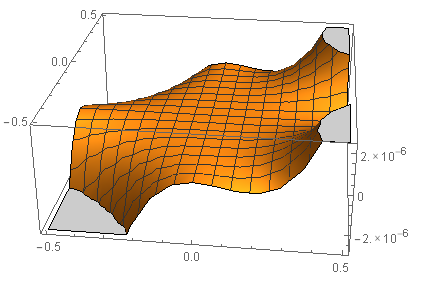
\includegraphics[scale=0.75]{upsilon}
%     %\caption{Caption}
%     %\label{fig:my_label}
% \end{figure}
% Bigger expansion:
% \begin{eqnarray*}
%     \Upsilon(x,y)
%     &=& \left(-\frac{i y^6}{576}+O\left(y^7\right)\right)
%     +x \left(\frac{i y^4}{1152}+\left(\frac{1}{9216}-\frac{i}{34560}\right)
%   y^6+O\left(y^7\right)\right)
%   +x^2 \left(-\frac{y^4}{2048}+\frac{y^6}{12288}+O\left(y^7\right)\right)
%   \\&&+x^3
%   \left(\left(\frac{1}{2304}+\frac{i}{576}\right) y^2-\left(\frac{1}{27648}+\frac{i}{6912}\right) y^4-\left(\frac{7}{414720}-\frac{7
%   i}{491520}\right) y^6+O\left(y^7\right)\right)\\
%   &&+x^4 \left(\left(\frac{23}{1152}-\frac{i}{288}\right)+\left(\frac{1}{18432}+\frac{43
%   i}{221184}\right) y^4-\left(\frac{1}{110592}+\frac{43 i}{1327104}\right) y^6+O\left(y^7\right)\right)\\
%   &&+x^5 \left(-\left(\frac{1}{9216}+\frac{79
%   i}{276480}\right) y^2+\left(\frac{1}{110592}+\frac{79 i}{3317760}\right) y^4+\left(\frac{479}{106168320}-\frac{1291 i}{398131200}\right)
%   y^6+O\left(y^7\right)\right)\\
%   &&+O\left(x^6\right)
% \end{eqnarray*}
% }


% \end{comment}
\end{document}